\documentclass[12pt,a4paper,twoside]{article}
\usepackage[T1]{fontenc}
\usepackage[utf8]{inputenc}
\usepackage[polish]{babel}
\usepackage{newtxtext,newtxmath}
\usepackage{amsmath}
\usepackage{booktabs}
\usepackage{graphicx}
\usepackage[a4paper,inner=30mm,outer=20mm,top=25mm,bottom=25mm]{geometry}
\usepackage{caption,subcaption}
\usepackage{float}
\usepackage{enumitem}
\usepackage{siunitx}
\usepackage{xcolor}
\usepackage{tikz}
\usetikzlibrary{arrows.meta}
\usepackage{setspace}
\usepackage{titlesec}
\usepackage{fancyhdr}
\usepackage{microtype}
\usepackage[hidelinks]{hyperref}

\setstretch{1.15}
\setlength{\parindent}{0.5cm}
\emergencystretch=1em
\sisetup{output-decimal-marker={,}}

\counterwithin{figure}{section}
\counterwithin{table}{section}

\DeclareCaptionFont{pwfont}{\fontsize{9}{11}\selectfont}
\captionsetup{font=pwfont,labelfont=bf,justification=raggedright,singlelinecheck=false}
\captionsetup[table]{position=top}
\captionsetup[figure]{position=bottom}

\titleformat{\section}[hang]{\fontsize{14}{17}\selectfont\bfseries}{\thesection}{0.6em}{}
\titleformat{\subsection}[hang]{\fontsize{13}{16}\selectfont\bfseries}{\thesubsection}{0.6em}{}
\titleformat{\subsubsection}[hang]{\fontsize{12}{15}\selectfont\bfseries}{\thesubsubsection}{0.6em}{}
\titlespacing*{\section}{0pt}{1.5em}{0.6em}
\titlespacing*{\subsection}{0pt}{1.2em}{0.4em}
\titlespacing*{\subsubsection}{0pt}{1.0em}{0.3em}

\fancypagestyle{plain}{%
	\fancyhf{}
	\renewcommand{\headrulewidth}{0pt}
	\fancyfoot[LE]{\thepage}
	\fancyfoot[RO]{\thepage}
}
\pagestyle{plain}

\begin{document}
\begin{titlepage}
	\begin{center}
		{\large POLITECHNIKA WARSZAWSKA\par}
		\vspace{0.8em}
		{\normalsize PRACA DYPLOMOWA INŻYNIERSKA\par}
		\vspace{2em}
		{\large\bfseries Analiza aerodynamiczna śmigła metodą BEMT jako analityczna weryfikacja symulacji ANSYS\par}
		\vspace{3em}
		{\Large Jakub Piotrowski\par}
		\vspace{1em}
		{\normalsize promotor: \underline{\hspace{7cm}}\par}
		\vfill
		{\normalsize WARSZAWA, 2026\par}
	\end{center}
\end{titlepage}

\setcounter{page}{1}
\begin{abstract}
	\begin{spacing}{1.0}
		\textbf{Analiza aerodynamiczna śmigła metodą BEMT jako analityczna weryfikacja symulacji ANSYS.}
		W pracy przedstawiono analizę aerodynamiczną dwułopatowego śmigła o średnicy \SI{0.5}{\meter}. Metoda elementu łopatkowego sprzężona z teorią pędu (BEMT) została zastosowana jako proste, analityczne narzędzie obliczeniowe do oceny rzędu wielkości sił i mocy przed porównaniem z wynikami CFD w środowisku ANSYS Fluent. Opisano geometrię, schemat domeny i siatki oraz konfigurację przygotowanej symulacji. Obliczenia BEMT wykonano dla prędkości lotu od \num{0} do \SI{30}{\meter\per\second} przy prędkości obrotowej \SI{3000}{rpm}.

		\noindent\textbf{Słowa kluczowe:} BEMT, CFD, ANSYS Fluent, śmigło, model turbulencji \(k-\omega\) SST, metoda MRF.
	\end{spacing}
\end{abstract}

\clearpage
\section*{Abstract}
\begin{spacing}{1.0}
	\textbf{Aerodynamic analysis of a propeller using the BEMT method as an analytical verification of ANSYS simulations.}
	The thesis presents an aerodynamic analysis of a two-blade propeller with a diameter of \SI{0.5}{\meter}. The blade element momentum theory (BEMT) was used as a simple analytical tool for estimating the order of magnitude of forces and power before comparing with the results of CFD simulations in the ANSYS Fluent environment. The geometry, the computational domain and mesh scheme, as well as the simulation setup are described. BEMT computations were performed for flight speeds from \num{0} to \SI{30}{\meter\per\second} at a rotational speed of \SI{3000}{rpm}.

	\noindent\textbf{Keywords:} BEMT, CFD, ANSYS Fluent, propeller, \(k-\omega\) SST turbulence model, MRF method.
\end{spacing}

\clearpage
\tableofcontents
\clearpage
	\section{Wstęp}
	Śmigła stanowią podstawowy element napędowy wielu statków powietrznych, dlatego ich charakterystyki aerodynamiczne podlegają ocenie już na etapie projektowania. Wyniki symulacji numerycznych CFD zależą między innymi od jakości siatki, warunków brzegowych oraz przyjętego modelu turbulencji, w związku z czym wymagają weryfikacji za pomocą niezależnego narzędzia obliczeniowego. W niniejszej pracy rolę takiego narzędzia pełni metoda elementu łopatkowego sprzężona z teorią pędu (BEMT), która pozwala w krótkim czasie oszacować rząd wielkości ciągu, momentu obrotowego i mocy wytwarzanych przez śmigło.
	
	Celem pracy jest analityczna weryfikacja symulacji CFD wykonanej w programie ANSYS Fluent na podstawie wyników obliczeń metodą BEMT. Przedstawiono geometrię dwułopatowego śmigła o średnicy \SI{0.5}{\meter}, sposób budowy domeny obliczeniowej i siatki oraz konfigurację solvera. Obliczenia BEMT przeprowadzono dla prędkości lotu od \num{0} do \SI{30}{\meter\per\second}, a symulacje CFD dla prędkości od 5 do \SI{30}{\meter\per\second}, w obu przypadkach przy stałej prędkości obrotowej \SI{3000}{rpm}. Uzyskane charakterystyki porównano, a zgodność obu metod oceniono w całym analizowanym zakresie, ze szczególnym uwzględnieniem zakresu pracy hamulcowej śmigła.
	\section{Geometria śmigła}
	Obiektem badań jest śmigło dwułopatowe (\(B=2\)) o promieniu \(R=\SI{0.25}{\meter}\). W obliczeniach BEMT przyjęto prędkość obrotową \(n=\SI{3000}{rpm}\) (\(\omega\approx\SI{314.16}{\radian\per\second}\)). Łopatę opisano zestawem stacji promieniowych; w każdej z nich określono profil, cięciwę oraz kąt skręcenia.
	\begin{table}[H]\centering
		\caption{Geometria łopaty: dane dla stacji promieniowych.}\label{tab:geometry}
		\begin{tabular}{cccccc}\toprule
			Stacja \(r/R\) & \(r\) [mm] & Profil & Cięciwa [mm] & \(\beta\) [\(^\circ\)] & Grubość wzgl. [\%] \\\midrule
			0,20 & 50 & NACA 4415 & 35 & 52 & 15 \\
			0,35 & 87,5 & NACA 4412 & 48 & 36 & 12 \\
			0,50 & 125 & NACA 4412 & 50 & 27 & 12 \\
			0,65 & 162,5 & NACA 4410 & 46 & 21 & 10 \\
			0,80 & 200 & NACA 4409 & 38 & 18 & 9 \\
			0,95 & 237,5 & NACA 4408 & 25 & 15 & 8 \\
			1,00 & 250 & NACA 4408 & 12 & 14 & 8 \\\bottomrule
	\end{tabular}\end{table}
	
	\begin{figure}[H]
		\centering
		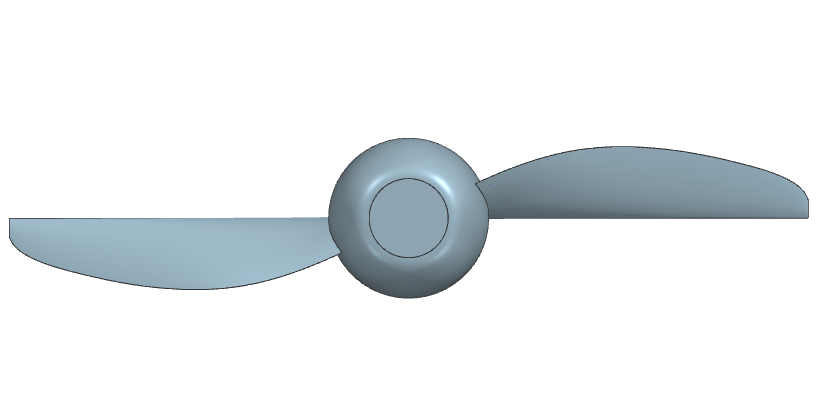
\includegraphics[width=1\linewidth]{geometria.png}
		\caption{Geometria śmigła.}
		\label{fig:geometry}
	\end{figure}
	\section{Model numeryczny: domena, siatka i przygotowanie symulacji}
	\subsection{Szkic geometrii i podział domeny}
	Model CFD składa się z dwóch współosiowych stref płynowych: nieruchomej domeny zewnętrznej oraz wewnętrznej domeny obrotowej obejmującej śmigło. Granica między nimi jest powierzchnią sprzężenia typu \textit{interface}. Wzdłuż kierunku przepływu wyznaczono wlot prędkościowy i wylot ciśnieniowy. Taki podział umożliwia uwzględnienie ruchu obrotowego bez fizycznego obracania siatki w analizie ustalonej.
	
	\subsection{Założenia siatkowania}
	Siatkę należy zagęścić w otoczeniu łopat, na krawędzi natarcia i spływu, przy końcówkach łopat oraz w śladzie za śmigłem. W warstwie przyściennej stosuje się warstwy pryzmatyczne, aby poprawnie odwzorować gradienty prędkości. Przejście między strefą obrotową i nieruchomą musi być zgodne z powierzchnią \textit{interface}; poza obszarami istotnymi aerodynamicznie dopuszczalne jest stopniowe rozrzedzenie siatki. Jakość rozwiązania należy ocenić przez niezależność wyników od zagęszczenia siatki, monitorując przede wszystkim ciąg i moment.
	
	\section{Metoda BEMT jako obliczenie referencyjne}
	Metoda BEMT (\textit{Blade Element Momentum Theory}) łączy opis lokalnego elementu łopaty z bilansem pędu strugi przechodzącej przez tarczę śmigła. W praktyce łopatę dzieli się na kilka pierścieniowych elementów. Dla każdego z nich, korzystając z geometrii oraz charakterystyk profilu, wyznacza się lokalne siły aerodynamiczne. Jednocześnie bilans pędu określa, jak śmigło zmienia prędkość powietrza.
	
	Jest to celowo uproszczony model: nie odwzorowuje pełnego trójwymiarowego przepływu tak jak CFD, ale szybko wskazuje oczekiwany rząd wielkości wyniku i trendy zmian. Dzięki temu może być używany jako proste obliczenie wykonywane ręcznie, a po zautomatyzowaniu jako krótki algorytm obliczeniowy. Jego wyniki będą punktem odniesienia podczas oceny symulacji Fluent.
	\subsection{Iteracyjny sposób działania}
	Dla każdego elementu promieniowego powtarza się następujący cykl:
	\begin{enumerate}[label=\arabic*.]
		\item Przyjmuje się początkowe wartości indukcji osiowej \(a\) i obwodowej \(a'\).
		\item Z prędkości lotu, prędkości obrotowej i przyjętej indukcji oblicza się lokalny napływ oraz kąt \(\varphi\).
		\item Z różnicy kąta ustawienia przekroju i kąta napływu wyznacza się kąt natarcia, a następnie odczytuje współczynniki nośności i oporu profilu.
		\item Na podstawie sił działających na element aktualizuje się wartości \(a\) i \(a'\), z uwzględnieniem strat końcowych w uproszczonej poprawce.
		\item Kroki powtarza się aż zmiany współczynników indukcji będą mniejsze od przyjętego progu zbieżności.
	\end{enumerate}
	Po uzyskaniu zbieżności sumuje się wkłady wszystkich elementów. Otrzymuje się ciąg \(T\), moment \(Q\), moc \(P\) i sprawność \(\eta\), które można bezpośrednio zestawić z wielkościami raportowanymi przez CFD.
	\section{Wyniki obliczeń analitycznych BEMT}
	Obliczenia BEMT wykonano dla \(V_\infty=0, 5, 10, 15, 20, 25\) i \SI{30}{\meter\per\second}. Wyniki w tabeli \ref{tab:global} stanowią zbiór referencyjny do porównania po ujednoliceniu parametrów obu modeli.
	\begin{table}[H]\centering
		\caption{Globalne parametry pracy śmigła obliczone metodą BEMT.}\label{tab:global}
		\begin{tabular}{cccccc}\toprule
			\(V_\infty\) [m/s] & \(T\) [N] & \(Q\) [Nm] & \(P\) [W] & \(\eta\) [-] & \(J\) [-] \\\midrule
			0 & 27,260 & 0,906 & 284,62 & 0,000 & 0,0000 \\
			5 & 25,364 & 1,037 & 325,73 & 0,389 & 0,2000 \\
			10 & 21,394 & 1,072 & 336,63 & 0,636 & 0,4000 \\
			15 & 15,105 & 0,919 & 288,76 & 0,785 & 0,6000 \\
			20 & 7,487 & 0,568 & 178,46 & 0,839 & 0,8000 \\
			25 & -1,505 & -0,035 & -11,06 & 0,000 & 1,0000 \\
			30 & -9,935 & -0,697 & -218,98 & 0,000 & 1,2000 \\\bottomrule
	\end{tabular}\end{table}
	Ciąg jest największy w warunkach statycznych i maleje ze wzrostem prędkości lotu. Dla najwyższych rozpatrywanych prędkości pojawia się wartość ujemna, co wskazuje na przejście do stanu wiatrakowania w przyjętym modelu.
	\begin{figure}[H]\centering
		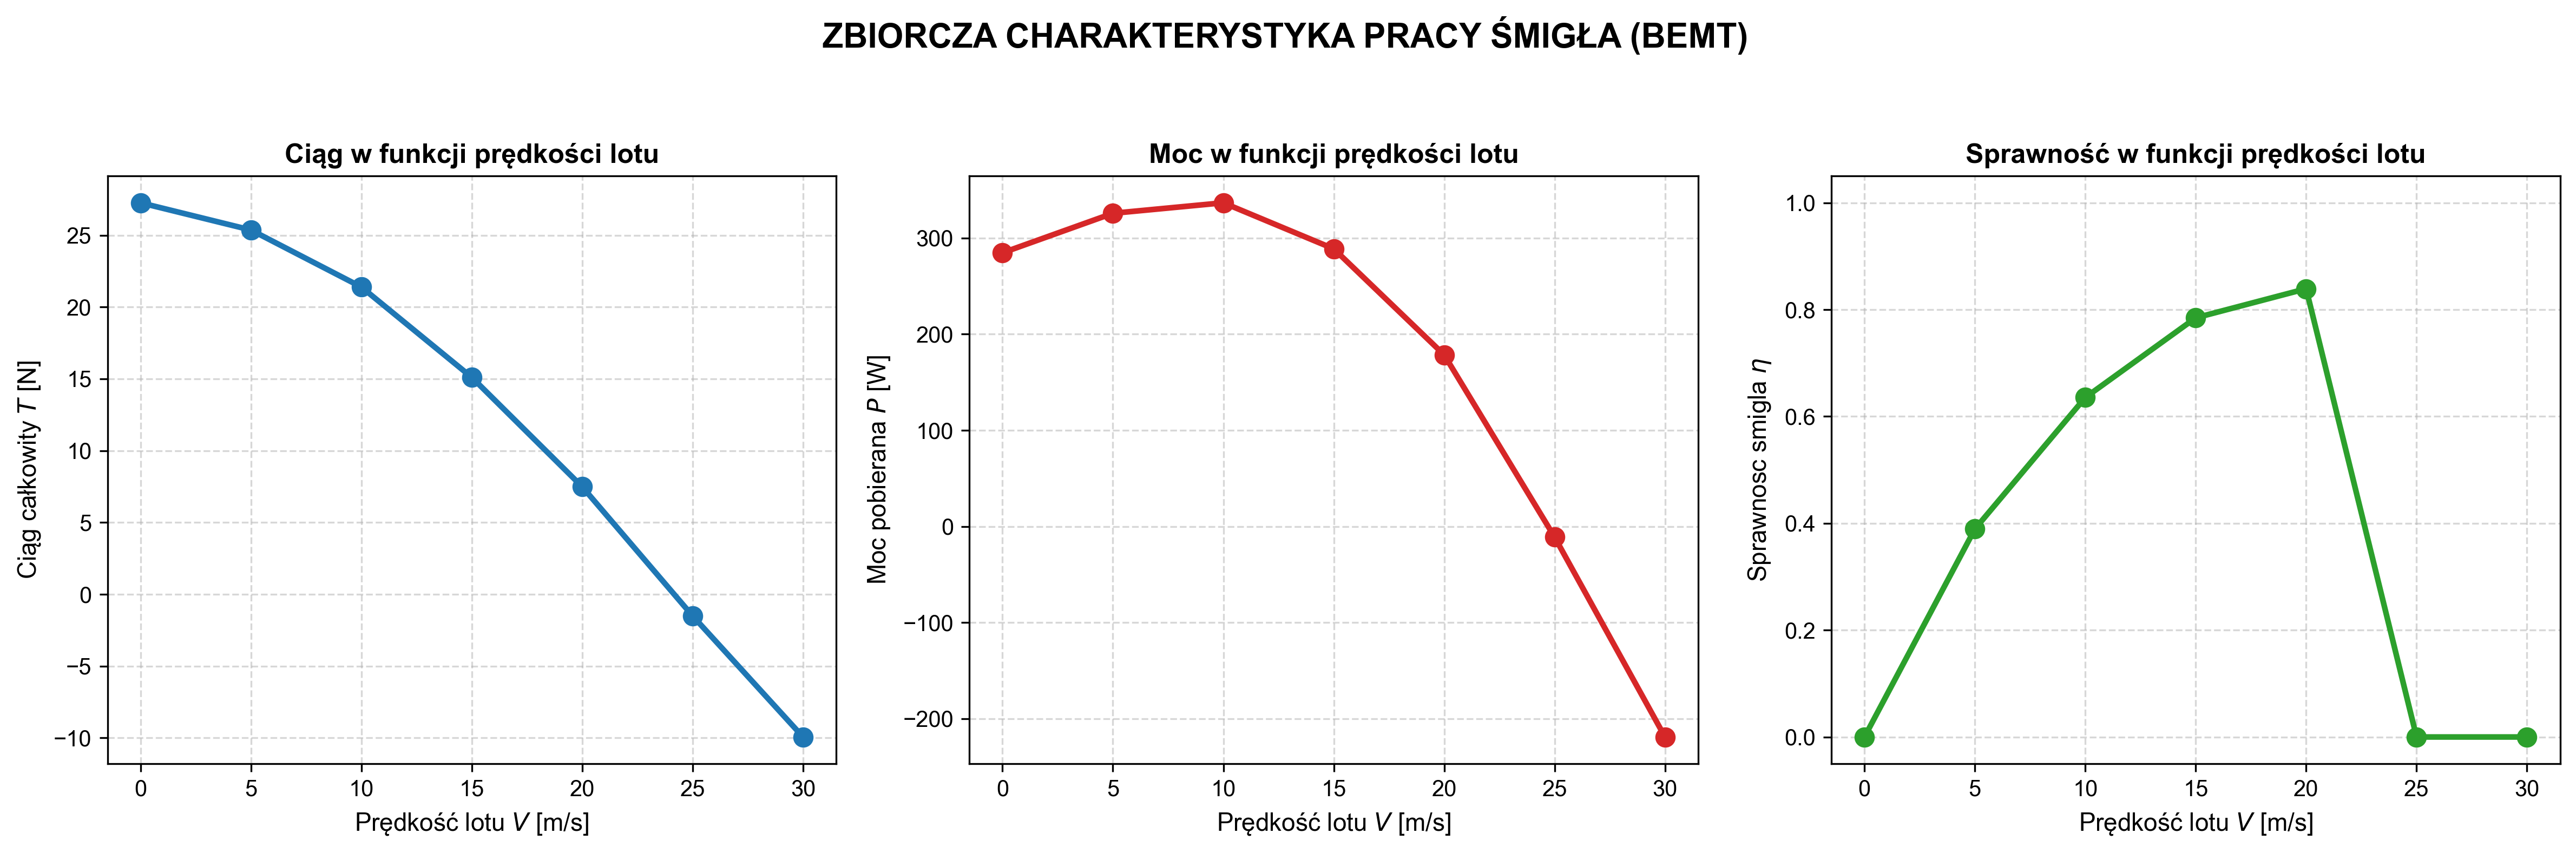
\includegraphics[width=.96\textwidth,height=.50\textheight,keepaspectratio]{podsumowanie_wynikow.png}
		\caption{Zbiorcze charakterystyki BEMT: ciąg, moc i sprawność w funkcji prędkości lotu.}\label{fig:summary}
	\end{figure}
	\begin{figure}[H]\centering
		\begin{subfigure}[b]{.49\textwidth}\centering
			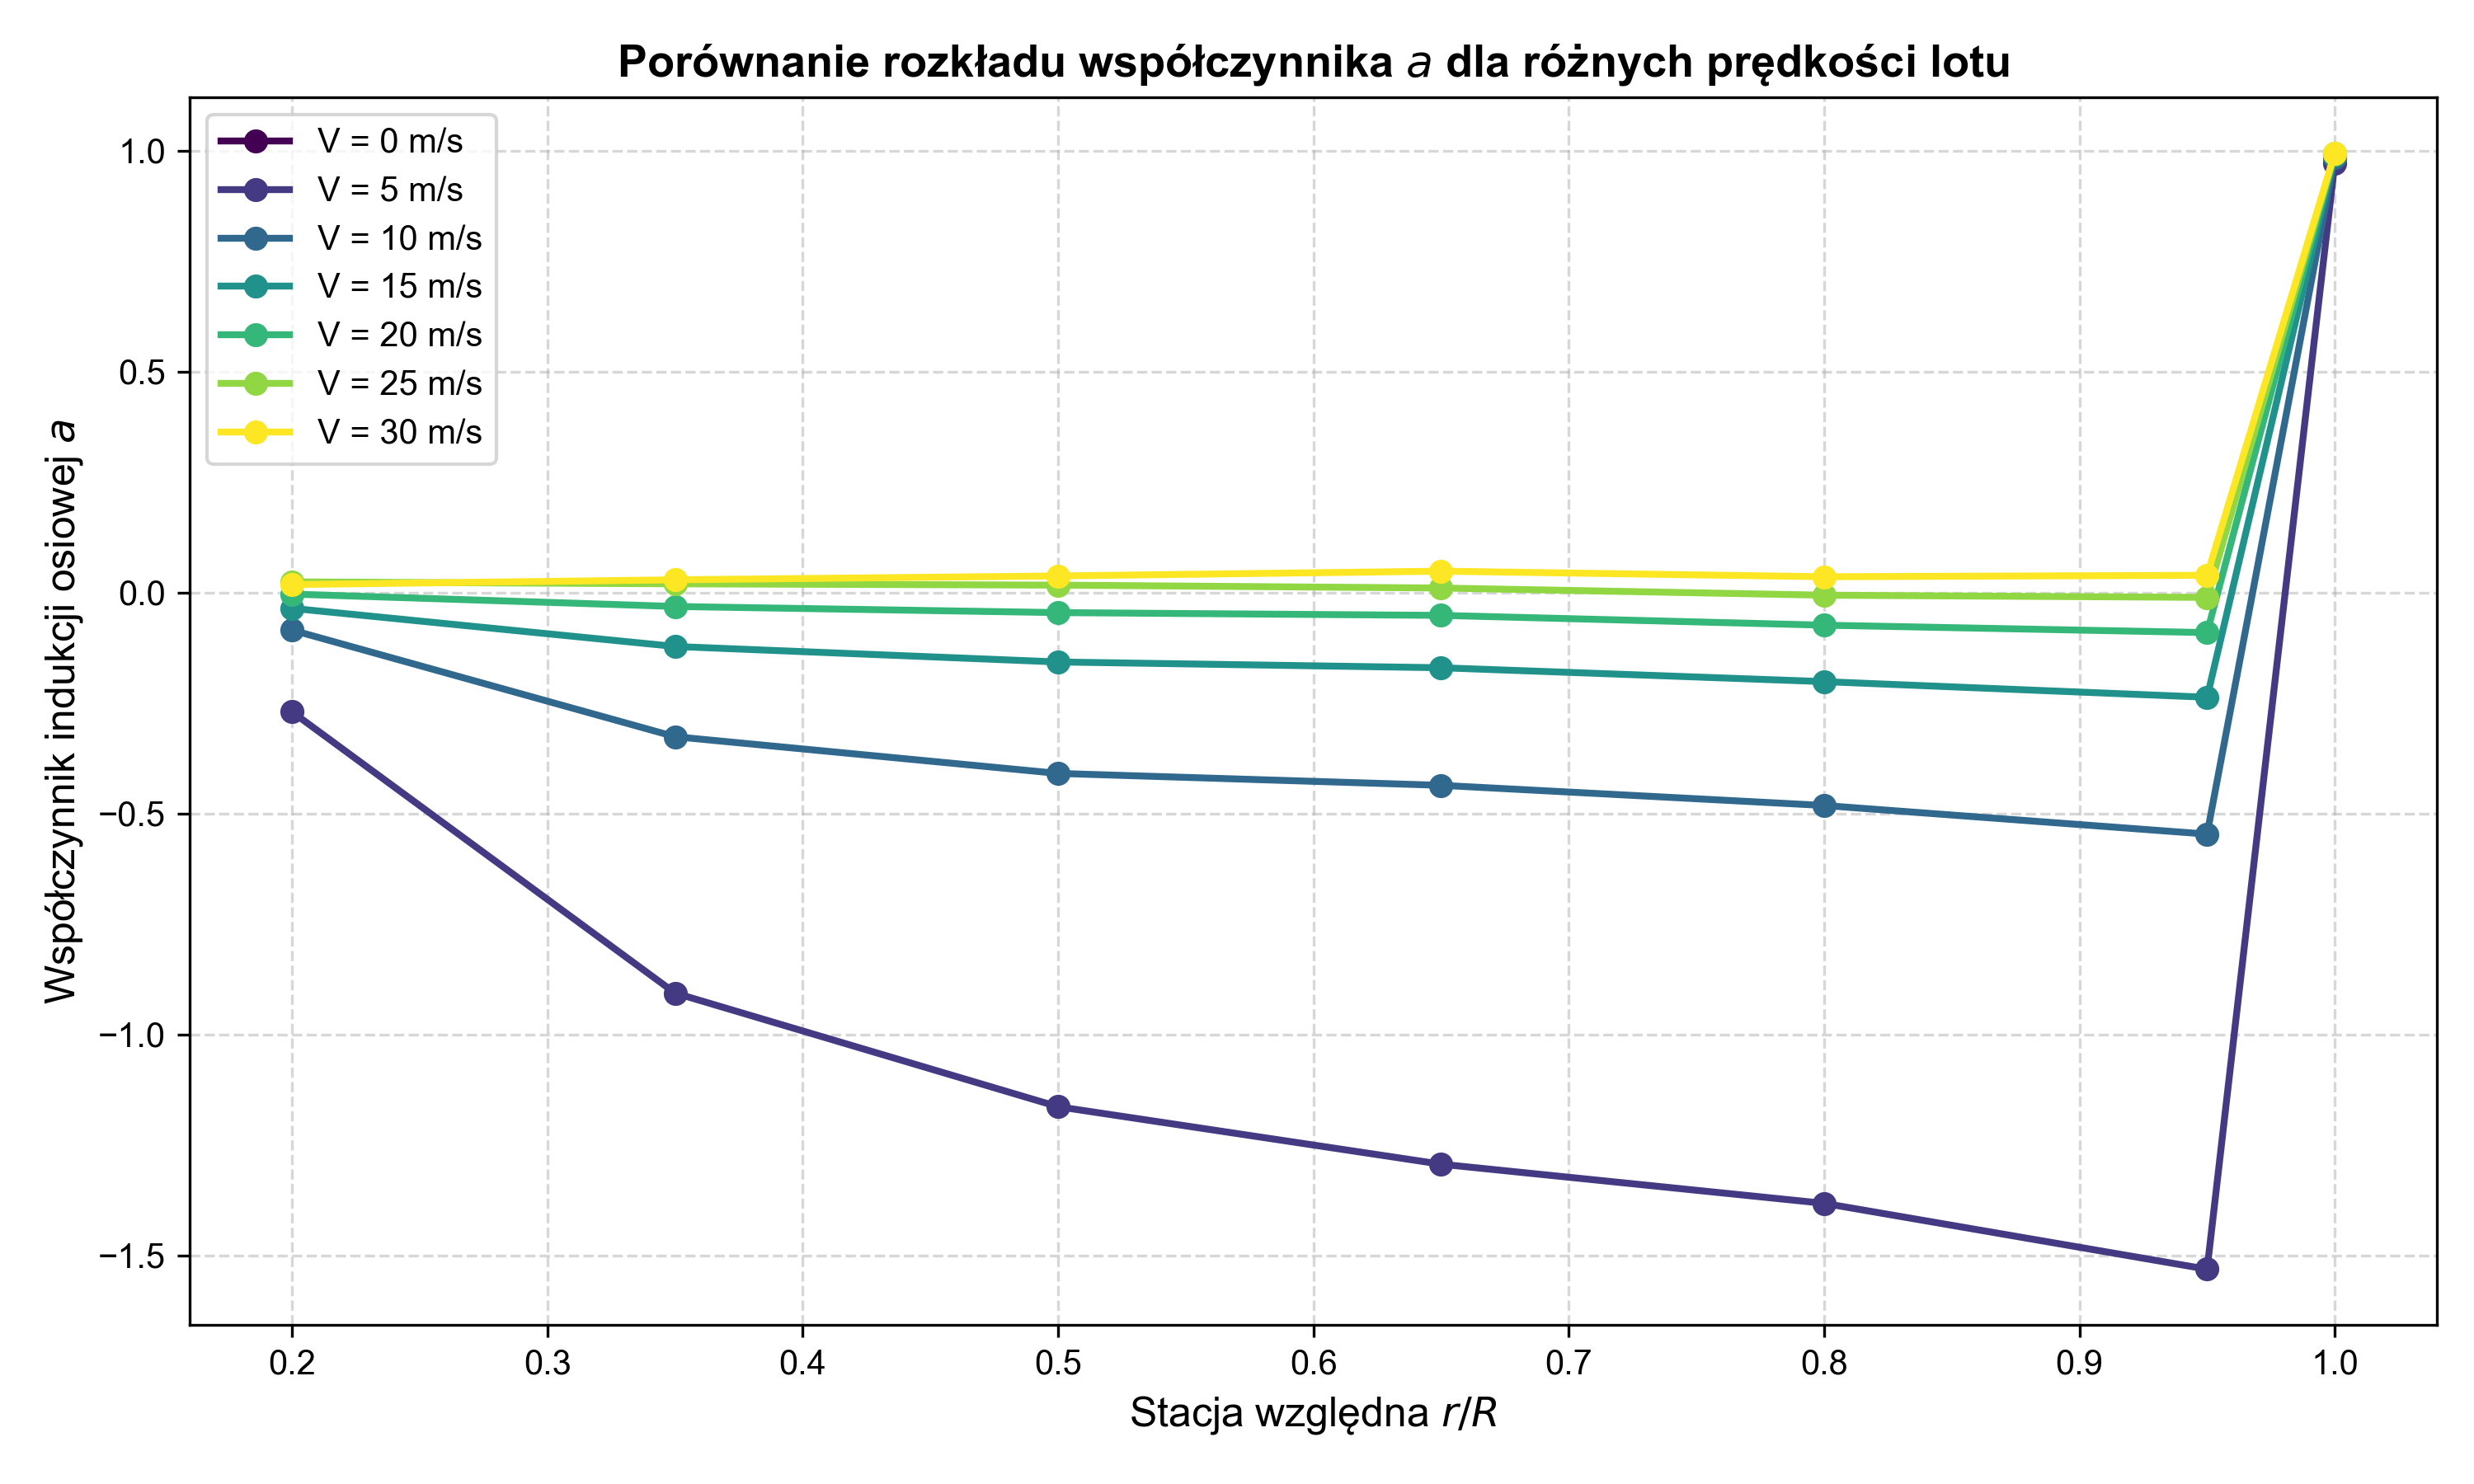
\includegraphics[width=\textwidth,height=.29\textheight,keepaspectratio]{porownanie_a.png}\caption{Współczynnik indukcji osiowej \(a\).}\end{subfigure}\hfill
		\begin{subfigure}[b]{.49\textwidth}\centering
			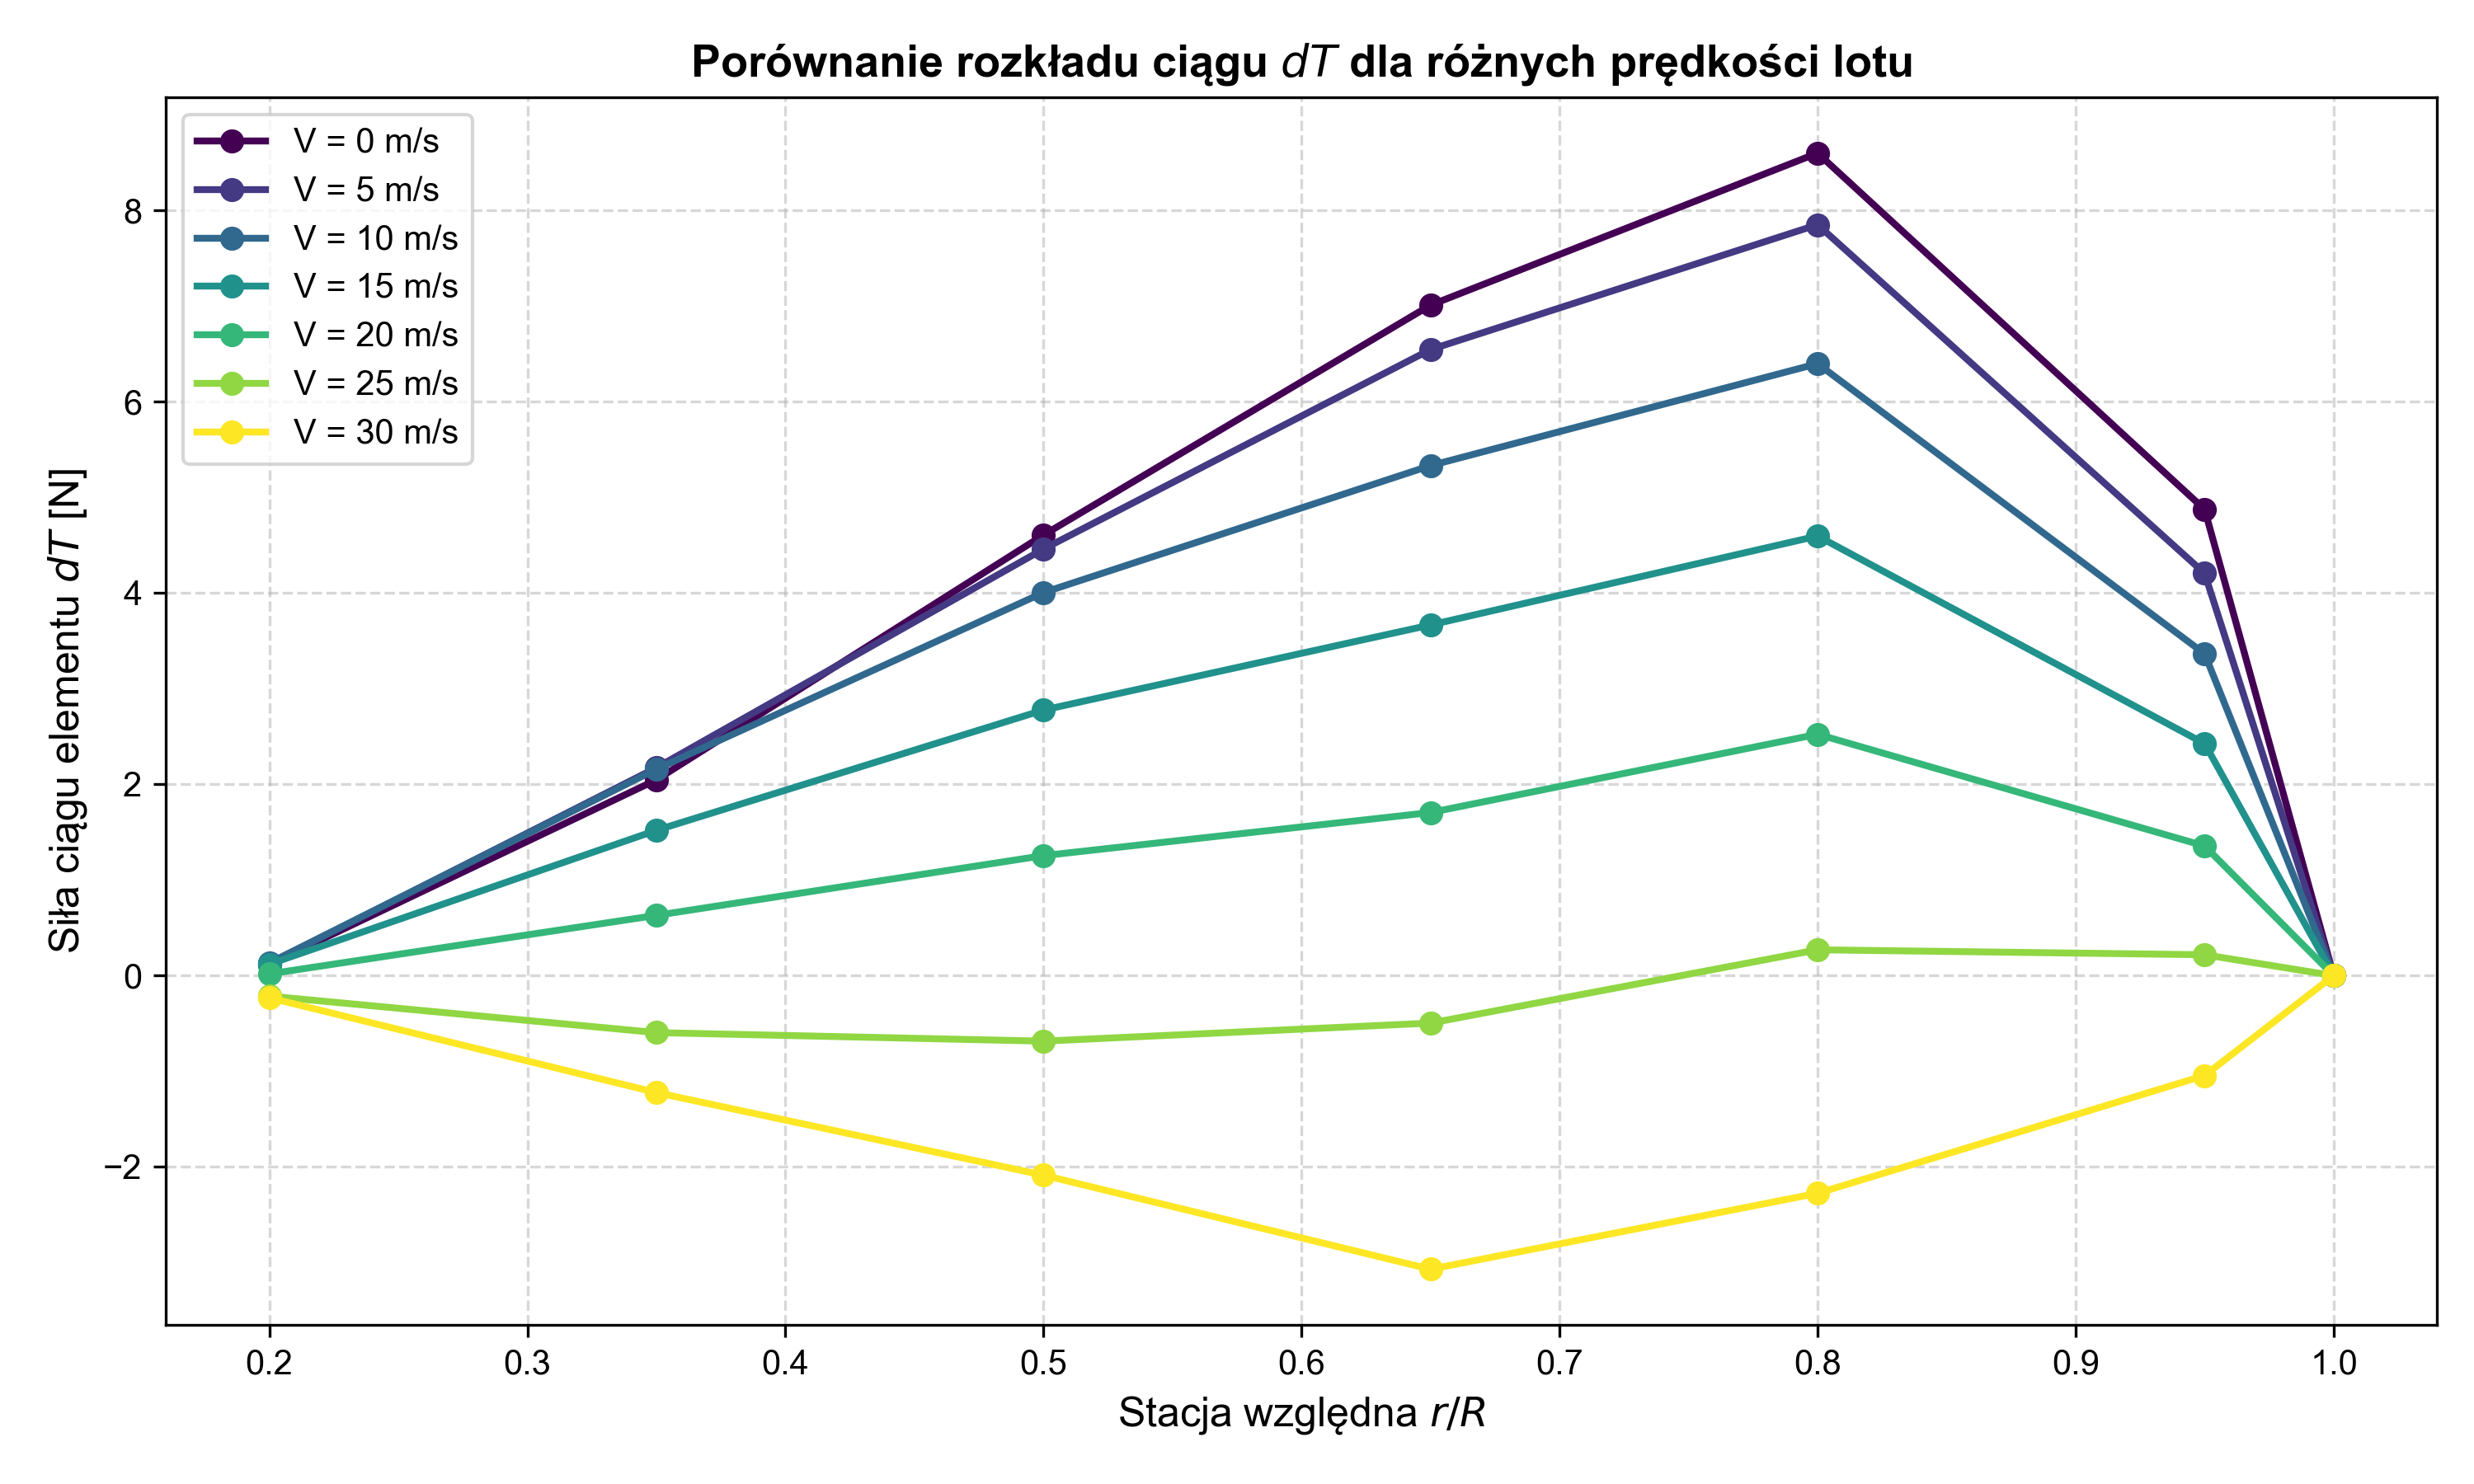
\includegraphics[width=\textwidth,height=.29\textheight,keepaspectratio]{porownanie_dT.png}\caption{Lokalny ciąg \(dT\).}\end{subfigure}
		\\[.8em]
		\begin{subfigure}[b]{.49\textwidth}\centering
			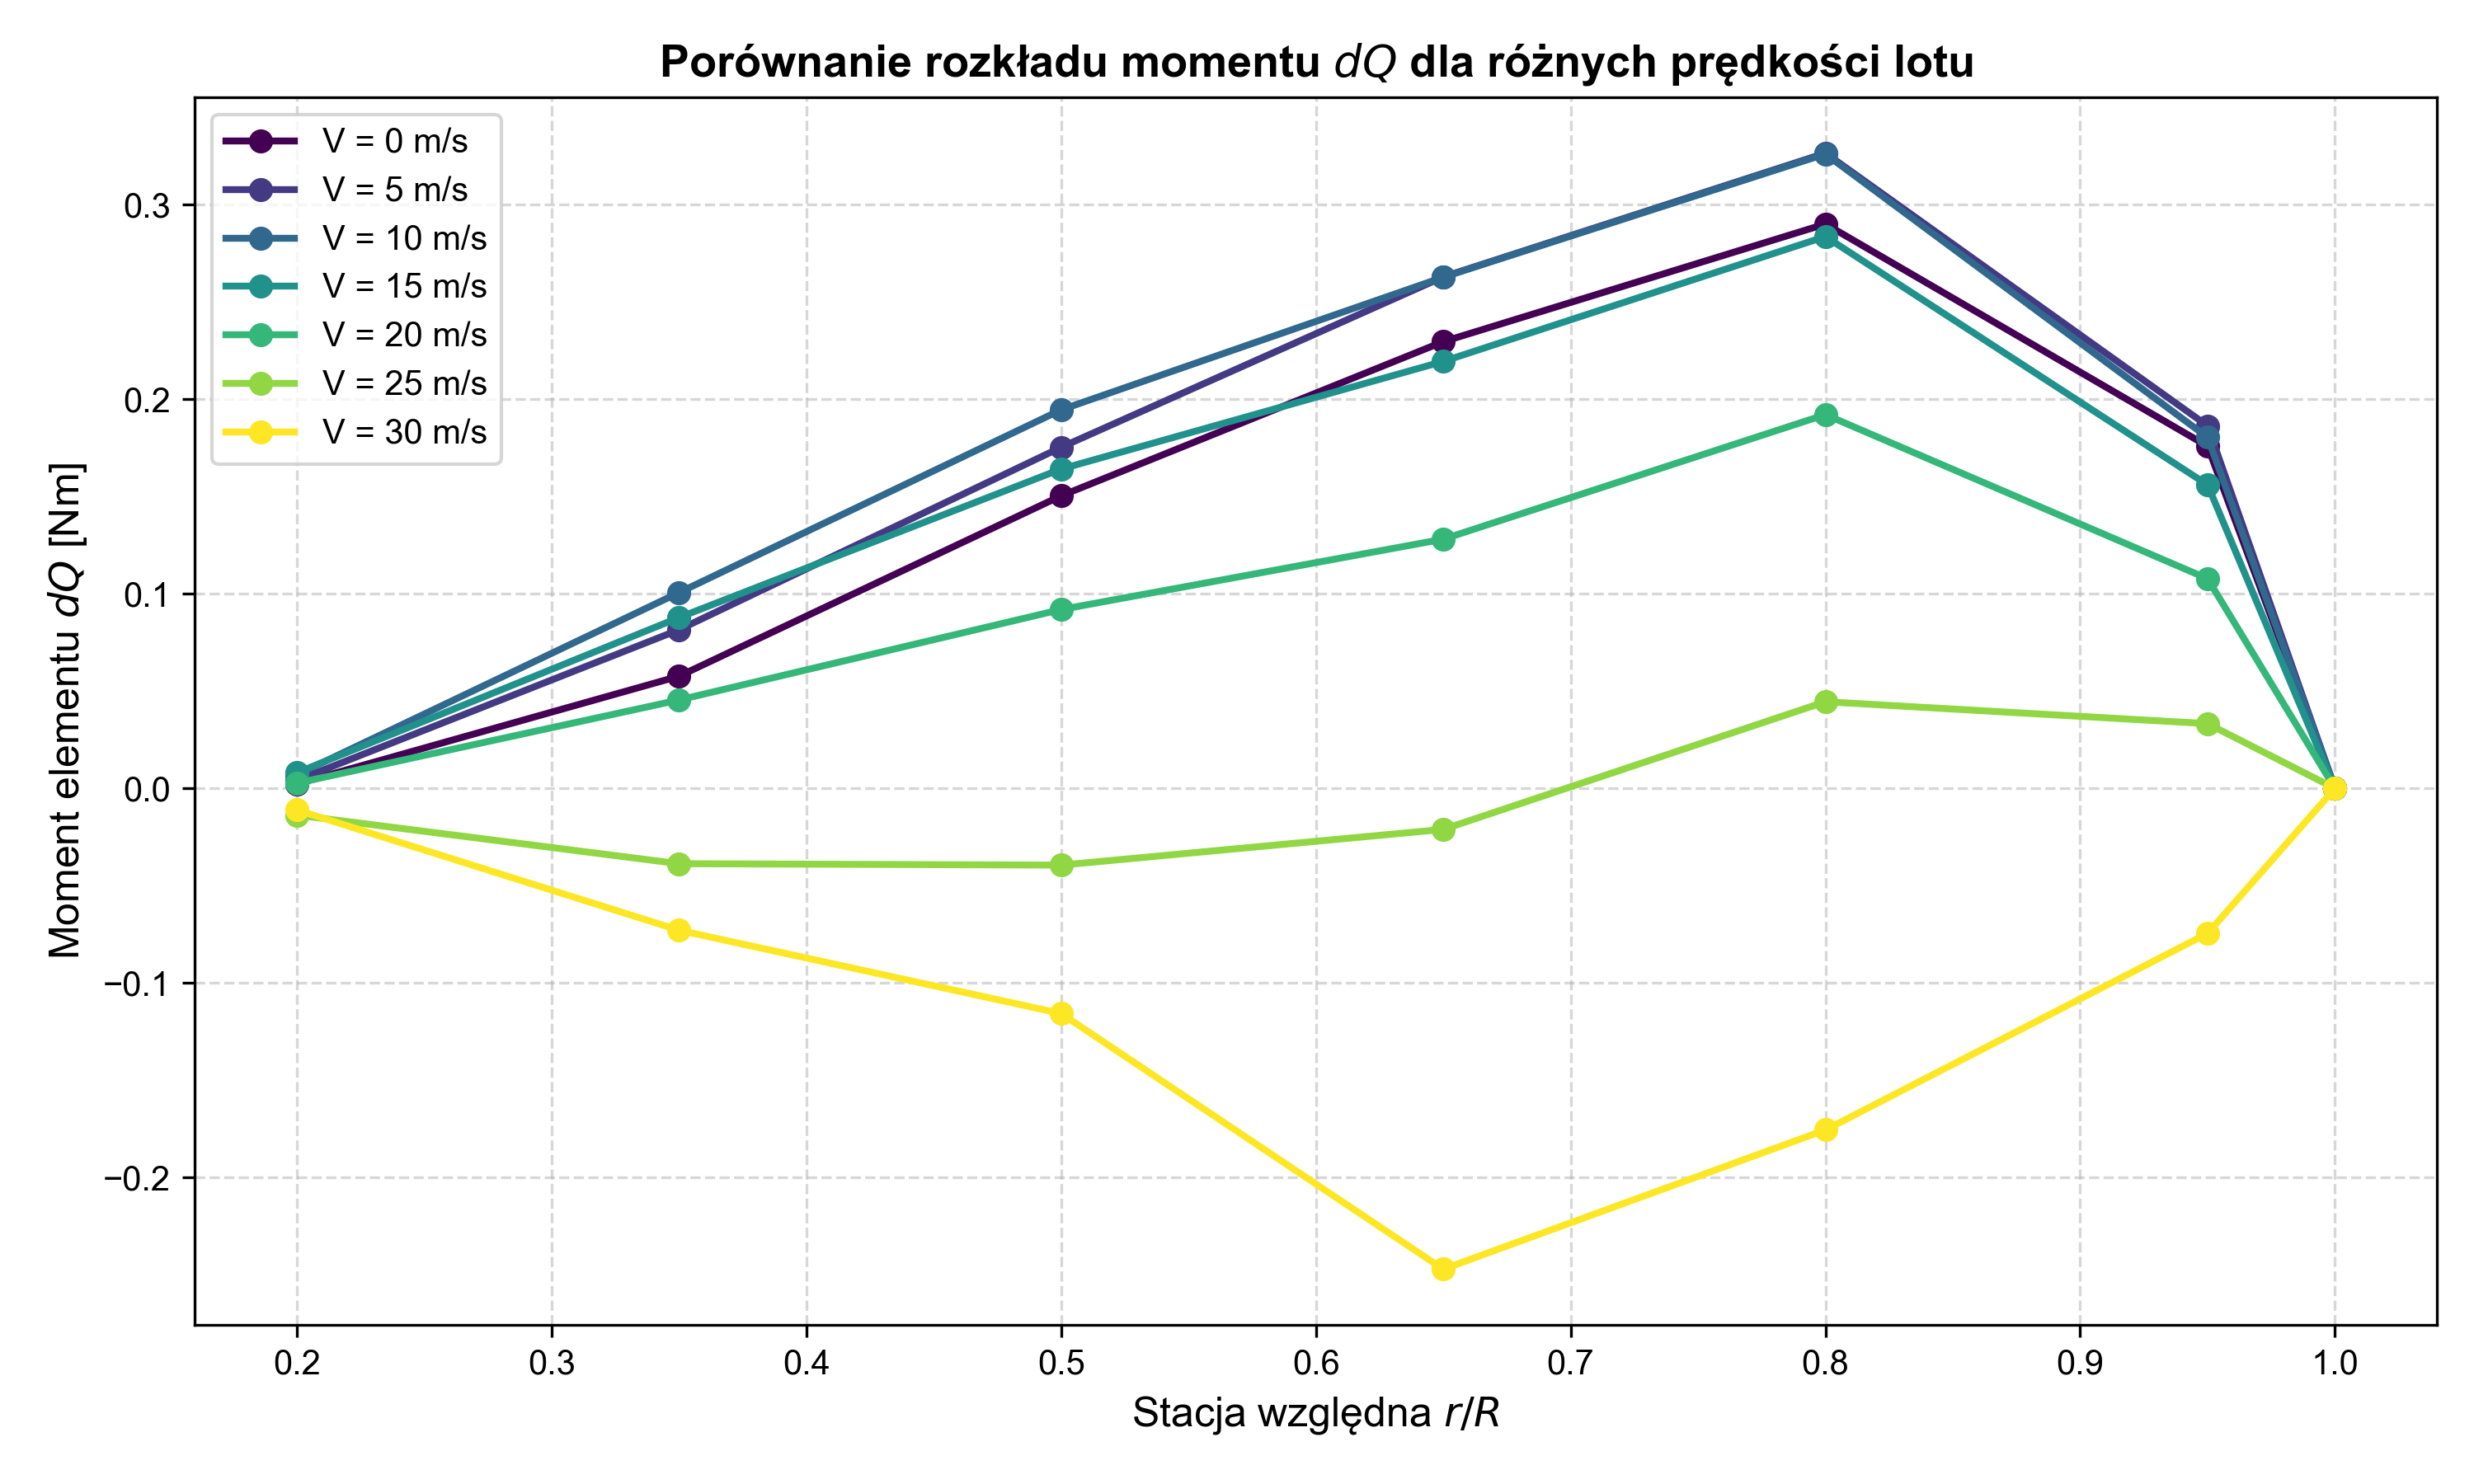
\includegraphics[width=\textwidth,height=.29\textheight,keepaspectratio]{porownanie_dQ.png}\caption{Lokalny moment \(dQ\).}\end{subfigure}
		\caption{Rozkłady lokalnych parametrów BEMT wzdłuż promienia dla analizowanych prędkości lotu.}\label{fig:local-comparison}
	\end{figure}
	\newpage
	\section{Model numeryczny CFD w programie ANSYS Fluent}
	
	\subsection{Wprowadzenie do symulacji}
	W celu bardziej szczegółowej analizy przepływu wokół śmigła oraz weryfikacji wyników uzyskanych metodą BEMT, wykonano symulację numeryczną w programie ANSYS Fluent 2026R1. Obliczenia przeprowadzono dla stałej prędkości obrotowej \SI{3000}{rpm} oraz zakresu prędkości lotu \(V_\infty = 5, 10, 15, 20, 25, 30\)~\si{\meter\per\second}. Wykorzystano metodę wirującego układu odniesienia (MRF, ang. Moving Reference Frame), która pozwala na symulację ruchu obrotowego śmigła w przepływie ustalonym (steady-state) przy znacznie niższym koszcie obliczeniowym w porównaniu z metodami nieustalonymi \cite{mrf_method}.
	
	\subsection{Domena obliczeniowa i siatka}
	
	\subsubsection{Geometria i podział domeny}
	Domena obliczeniowa została podzielona na dwa obszary:
	\begin{itemize}
		\item \textbf{Strefa wirująca (MRF)} walec o średnicy \SI{0.55}{\meter} (1.1 średnicy śmigła), ściśle otaczający łopaty, w którym zdefiniowano wirujący układ odniesienia,
		\item \textbf{Strefa stacjonarna} walec o średnicy \SI{4}{\meter} (8 średnic śmigła), oraz wysokości \SI{5}{\meter} obejmujący strefę wirującą, reprezentujący dalekie pole przepływu.
	\end{itemize}
	Ze względu na symetrię okresową śmigła dwułopatowego zamodelowano wycinek kątowy \SI{180}{\degree} zawierający jedną łopatę. Zastosowanie symetrii okresowej pozwoliło na redukcję liczby elementów siatki o połowę i usprawnienie obliczeń.
	
	\subsubsection{Parametry siatki}
	Siatkę wygenerowano w module \texttt{Mesh} programu ANSYS Workbench. Zastosowano siatkę niestrukturalną typu \texttt{Poly-Hexcore}, która zapewnia wysoką ortogonalność przy zredukowanej liczbie elementów. Kluczowe parametry siatki zestawiono w tabeli \ref{tab:mesh_params_cfd}.
	
	\begin{table}[H]
		\centering
		\caption{Zestawienie parametrów siatki obliczeniowej.}
		\label{tab:mesh_params_cfd}
		\begin{tabular}{@{}l r@{}}
			\toprule
			\textbf{Parametr} & \textbf{Wartość} \\
			\midrule
			Całkowita liczba elementów & $\approx$ 800 tys. \\
			Liczba elementów strefa MRF & $\approx$ 300 tys. \\
			Liczba elementów strefa stacjonarna & $\approx$ 500 tys. \\
			Rozmiar elementu powierzchnia łopaty (Face Sizing) & \SI{2.5}{\milli\meter} \\
			Rozmiar elementu strefa MRF (Body Sizing) & \SI{9}{\milli\meter} \\
			Rozmiar elementu strefa stacjonarna (Body Sizing) & \SI{120}{\milli\meter} \\
			Liczba warstw przyściennych (Inflation) & 5 \\
			Grubość całkowita warstwy przyściennej & \SI{1}{\milli\meter} \\
			Współczynnik wzrostu (Growth Rate) & 1,2 \\
			\bottomrule
		\end{tabular}
	\end{table}
	
	\subsubsection{Jakość siatki}
	Jakość siatki oceniono na podstawie dwóch kluczowych wskaźników: zniekształcenia (Skewness) oraz ortogonalności (Orthogonal Quality). Zgodnie z zaleceniami dla obliczeń CFD, maksymalne zniekształcenie powinno być utrzymywane poniżej 0,95, a minimalna ortogonalność powyżej 0,1 \cite{ansys_mesh_quality}. Uzyskane wartości przedstawiono w tabeli \ref{tab:mesh_quality_cfd}.
	
	\begin{table}[H]
		\centering
		\caption{Metryki jakości siatki.}
		\label{tab:mesh_quality_cfd}
		\begin{tabular}{@{}p{4.8cm} c c@{}}
			\toprule
			\textbf{Metryka} & \textbf{Uzyskana wartość} & \textbf{Zalecana wartość} \\
			\midrule
			Maksymalne zniekształcenie (Skewness) & 0,9414 & $< 0{,}95$ \\
			Minimalna ortogonalność (Orthogonal Quality) & 0,04523 & $> 0{,}1$ \\
			\bottomrule
		\end{tabular}
	\end{table}
	
	Należy podkreślić, że wartość minimalnej ortogonalności (0,045) jest niższa od zalecanej. Jest to wynikiem kompromisu pomiędzy jakością siatki a ograniczeniem liczby elementów do ok. 1 miliona. Mimo to symulacje wykazały stabilną zbieżność, co sugeruje, że lokalnie słaba jakość siatki nie wpłynęła znacząco na wyniki.
	
	
	\begin{figure}[H]
		\centering
		
\includegraphics[width=1\linewidth]{mesh_rational.png}
		\caption{Zdjęcie siatki strefy wirującej (domena obrotowa).}
		\label{fig:mesh-rotating}
	\end{figure}
	
	\begin{figure}[H]
		\centering
		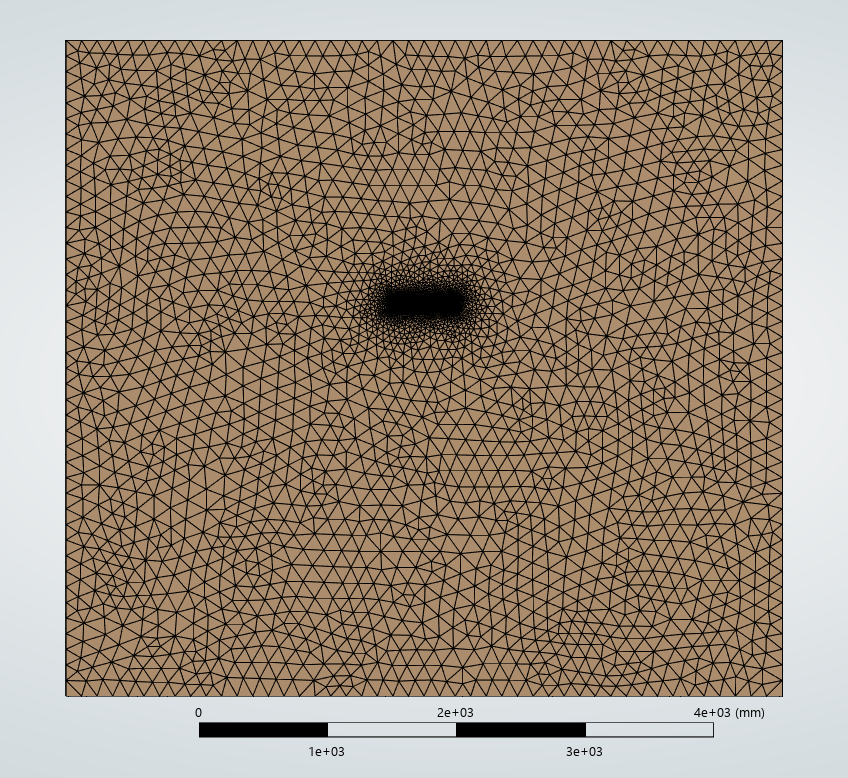
\includegraphics[width=0.6\linewidth]{mesh.png}
		\caption{Widok siatki całej geometrii.}
		\label{fig:mesh-overall}
	\end{figure}
	
	\subsection{Model fizyczny i ustawienia solvera}
	
	\subsubsection{Model turbulencji}
	Do zamknięcia równań Reynoldsa (RANS) wykorzystano model turbulencji \(k-\omega\) SST (Shear Stress Transport). Model ten został wybrany ze względu na jego lepszą zdolność do przewidywania przepływów z separacją i silnymi gradientami ciśnienia, które występują wokół łopat śmigła \cite{menter1994}. Dodatkowo, badania wskazują, że dobór modelu turbulencji oraz typu siatki istotnie wpływa na dokładność przewidywania charakterystyk śmigła \cite{sikirica2019}, a architektura \(k-\omega\) SST dobrze sprawdza się w przypadku małych śmigieł o niskiej liczbie Reynoldsa \cite{kutty2017}.
	
	\subsubsection{Ustawienia solvera}
	Główne ustawienia solvera w ANSYS Fluent zestawiono w tabeli \ref{tab:solver_setup_cfd}.
	
	\begin{table}[H]
		\centering
		\caption{Ustawienia solvera ANSYS Fluent.}
		\label{tab:solver_setup_cfd}
		\begin{tabular}{@{}l l@{}}
			\toprule
			\textbf{Parametr} & \textbf{Wartość} \\
			\midrule
			Typ solvera & Pressure-Based \\
			Przepływ & Ustalony (Steady) \\
			Precyzja & Podwójna (Double Precision) \\
			Model turbulencji & \(k-\omega\) SST \\
			Traktowanie ścian & Automatic Wall Treatment \\
			Schemat dyskretyzacji pędu & Second Order Upwind \\
			Schemat dyskretyzacji turbulencji & First Order Upwind \\
			%Współczynnik relaksacji ciśnienia & 0.1 \\
			%Współczynnik relaksacji pędu & 0.3 \\
			%Współczynnik relaksacji turbulencji & 0.4 \\
			\bottomrule
		\end{tabular}
	\end{table}
	
	\subsection{Warunki brzegowe}
	Warunki brzegowe zdefiniowano zgodnie z poniższym zestawieniem:
	\begin{itemize}
		\item \textbf{Wlot (Inlet)}: \texttt{Velocity Inlet} z prędkością \(V_\infty = 5, 10, 15, 20, 25, 30\)~\si{\meter\per\second}. Intensywność turbulencji: 5\%, stosunek lepkości turbulentnej: 10.
		\item \textbf{Wylot (Outlet)}: \texttt{Pressure Outlet} z ciśnieniem manometrycznym 0 Pa.
		\item \textbf{Ściana boczna domeny stacjonarnej}: \texttt{Symmetry}  eliminacja wpływu lepkości ścian zewnętrznych na przepływ.
		\item \textbf{Powierzchnia łopatek śmigła}: \texttt{Wall} z warunkiem braku poślizgu i zerową prędkością względną w strefie wirującej.
		
	\end{itemize}
	
	\subsection{Metoda MRF (Moving Reference Frame)}
	Ruch obrotowy śmigła zamodelowano za pomocą metody MRF \cite{mrf_method}. W strefie wirującej zdefiniowano prędkość obrotową \(n = 3000\) RPM wokół osi Z. Metoda MRF pozwala na przeprowadzenie symulacji ustalonej, co znacząco redukuje koszt obliczeniowy w porównaniu z metodami nieustalonymi.
	
	\subsection{Proces zbieżności i monitoring}
	
	\subsubsection{Monitory obliczeń}
	W celu kontroli zbieżności rozwiązania utworzono następujące monitory:
	\begin{itemize}
		\item \textbf{Residua} dla równań ciągłości, pędu (\(x\), \(y\), \(z\)) oraz turbulencji (\(k\), \(\omega\)),
		\item \textbf{Force Monitor} śledzący siłę ciągu w osi Z na powierzchni łopatek,
		\item \textbf{Surface Monitor} monitorujący średnie ciśnienie statyczne (Area-Weighted Average) na powierzchni łopatek.
	\end{itemize}
	\subsubsection{Przebieg zbieżności}
	Symulację dla każdego punktu pracy przeprowadzono do momentu uzyskania stabilizacji monitorów sił. Przykładowy przebieg residuów oraz monitorów dla prędkości \(V_\infty = 5\)~\si{\meter\per\second} przedstawiono na rysunkach \ref{fig:residuals_cfd} oraz \ref{fig:pressure_cfd}.
	
	\begin{figure}[H]
		\centering
		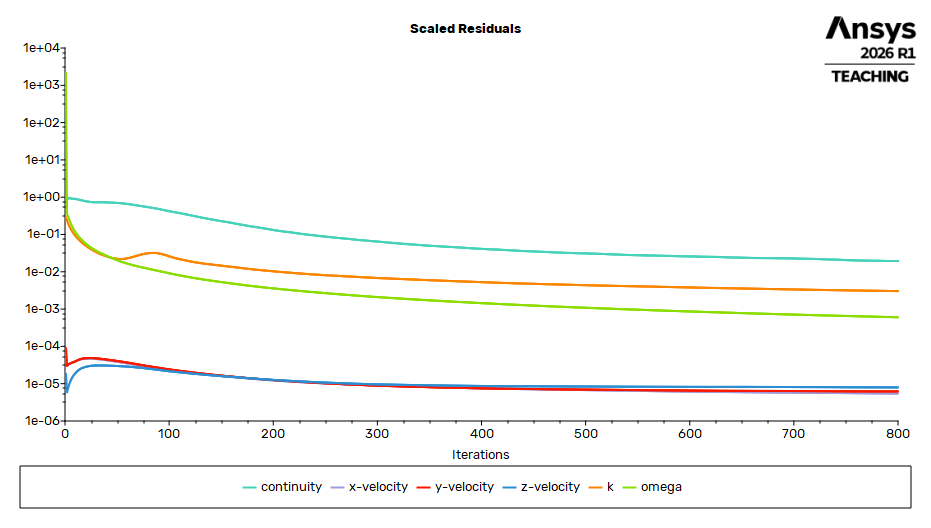
\includegraphics[width=1\textwidth]{residuals_25ms.png}
		\caption{Przebieg residuów dla \(V_\infty = 5\) m/s, \(n = 3000\) RPM.}
		\label{fig:residuals_cfd}
	\end{figure}
	
	Po niecałych 700 iteracjach wszystkie residua osiągnęły stabilny poziom: $\approx 1\times10^{-3}$.
	
	\begin{figure}[H]
		\centering
		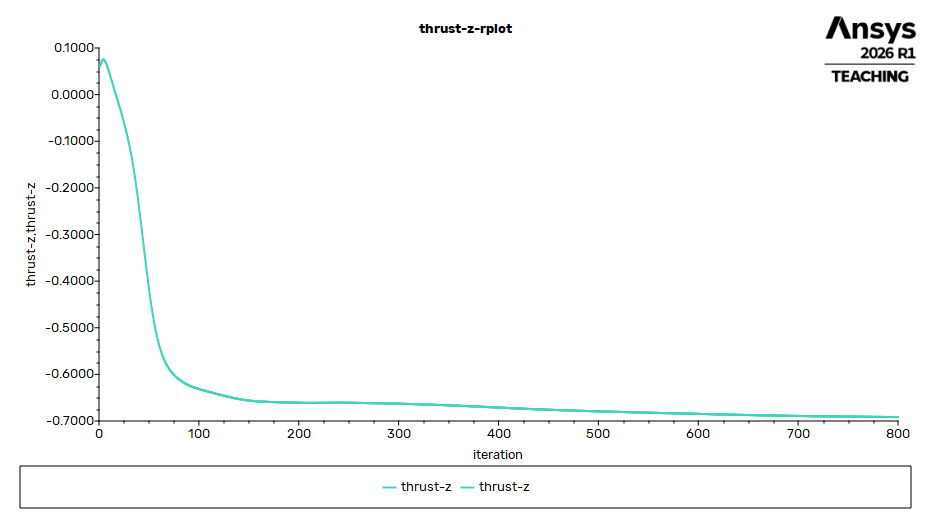
\includegraphics[width=1\textwidth]{thrust_25ms.png}
		\caption{Przebieg ciągu (Thrust) dla \(V_\infty = 5\) m/s, \(n = 3000\) RPM.}
		\label{fig:thrust_cfd}
	\end{figure}
	
	Wykres ciągu (rys. \ref{fig:thrust_cfd}) osiągnął plateau po ok. 300 iteracjach, co potwierdza osiągnięcie stanu ustalonego.
	
	\begin{figure}[H]
		\centering
		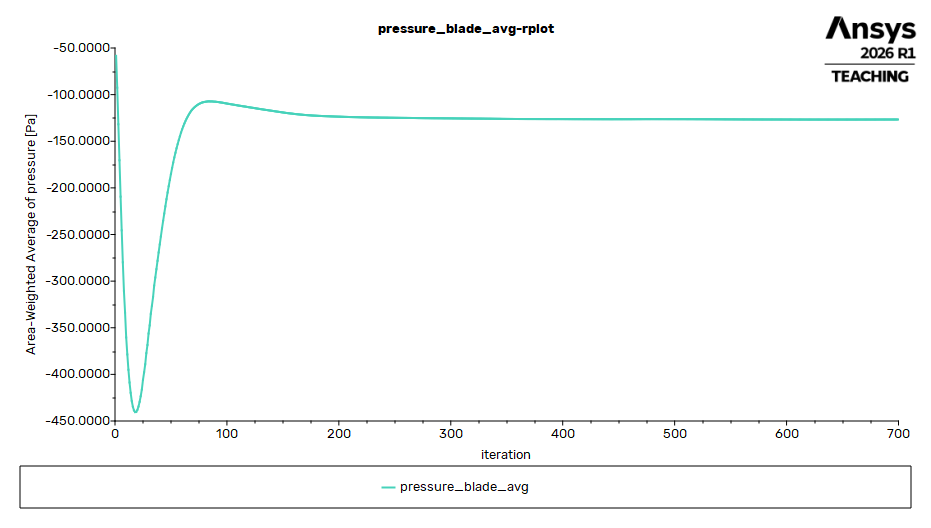
\includegraphics[width=1\textwidth]{pressure_25ms.png}
		\caption{Średnie ciśnienie statyczne na łopatce dla \(V_\infty = 5\) m/s.}
		\label{fig:pressure_cfd}
	\end{figure}
	
	Średnie ciśnienie statyczne na powierzchni łopatki (rys. \ref{fig:pressure_cfd}) ustabilizowało się na poziomie ok. \SI{-300}{\pascal}, co jest wartością fizycznie poprawną.
	
	\subsection{Wyniki symulacji CFD}
	
	\subsubsection{Charakterystyka ciągu}
	Wartości ciągu dla poszczególnych prędkości napływu zestawiono w tabeli \ref{tab:thrust_results_cfd}. Zgodnie z uwagą do danych źródłowych, wartości siły i momentu obrotowego z modelu połowy śmigła przeliczono na pełne śmigło (mnożąc dane z wyniku symulacji dwukrotnie); kolumna ,,połówka'' podaje surowe wartości z modelu połówkowego.
	
	\begin{table}[H]
		\centering
		\caption{Wyniki ciągu z symulacji CFD dla \(n = 3000\) RPM.}
		\label{tab:thrust_results_cfd}
		\begin{tabular}{@{}c c c@{}}
			\toprule
			\textbf{Prędkość napływu} & \textbf{CFD (połówka)} & \textbf{CFD (całość)} \\
			\(V_\infty\) [m/s] & \(T\) [N] & \(T\) [N] \\
			\midrule
			0  & 9,54  & 19,08 \\
			5  & 7,24  & 14,48 \\
			10 & 6,37  & 12,74 \\
			15 & 4,42  & 8,84  \\
			20 & 1,37  & 2,74  \\
			25 & -2,00 & -4,00 \\
			30 & -4,64 & -9,28 \\
			\bottomrule
		\end{tabular}
	\end{table}
	
	Ciąg śmigła maleje monotonicznie wraz ze wzrostem prędkości napływu. W warunkach statycznych (\(V_\infty = 0\) m/s) śmigło wytwarza największy ciąg (19,08 N), który przy \(V_\infty = 20\) m/s spada do 2,74 N, a powyżej tej prędkości zmienia znak na ujemny. Przejście w stan wiatrakowania (tryb hamulcowy) dla \(V_\infty \ge 25\) m/s jest fizycznie poprawnym zachowaniem śmigła i zostało odtworzone przez symulację.
	
	\subsubsection{Charakterystyka momentu obrotowego}
	Wartości momentu obrotowego dla poszczególnych prędkości napływu zestawiono w tabeli \ref{tab:torque_results_cfd}.
	
	\begin{table}[H]
		\centering
		\caption{Wyniki momentu obrotowego z symulacji CFD dla \(n = 3000\) RPM.}
		\label{tab:torque_results_cfd}
		\begin{tabular}{@{}c c c@{}}
			\toprule
			\textbf{Prędkość napływu} & \textbf{CFD (połówka)} & \textbf{CFD (całość)} \\
			\(V_\infty\) [m/s] & \(Q\) [Nm] & \(Q\) [Nm] \\
			\midrule
			0  & 0,29    & 0,580    \\
			5  & 0,32    & 0,640    \\
			10 & 0,40    & 0,800    \\
			15 & 0,33    & 0,660    \\
			20 & 0,21    & 0,420    \\
			25 & -0,017  & -0,033   \\
			30 & -0,099  & -0,199   \\
			\bottomrule
		\end{tabular}
	\end{table}
	
	Moment obrotowy rośnie w zakresie małych prędkości napływu i osiąga maksimum przy \(V_\infty = 10\) m/s (0,80 Nm), po czym maleje wraz ze wzrostem prędkości. W miarę przechodzenia śmigła w stan hamowania jego wartość spada poniżej zera. Wraz ze spadkiem momentu obrotowego zmniejsza się również moc potrzebna do napędu śmigła.
	
	\subsubsection{Moc i sprawność}
	Na podstawie uzyskanych wartości momentu obrotowego oraz siły ciągu wyznaczono moc pobieraną przez śmigło i jego sprawność. Wyniki zestawiono w tabeli \ref{tab:power_efficiency_cfd}.
	
	\begin{table}[H]
		\centering
		\caption{Moc i sprawność śmigła z symulacji CFD dla \(n = 3000\) RPM.}
		\label{tab:power_efficiency_cfd}
		\begin{tabular}{@{}c c c@{}}
			\toprule
			\textbf{Prędkość napływu} & \textbf{Moc} & \textbf{Sprawność} \\
			\(V_\infty\) [m/s] & \(P\) [W] & \(\eta\) [\%] \\
			\midrule
			0  & 174,00   & 0,0   \\
			5  & 192,00   & 37,7  \\
			10 & 239,92   & 53,1  \\
			15 & 198,00   & 67,0  \\
			20 & 126,00   & 43,5  \\
			25 & -9,99    & 0,0   \\
			30 & -59,65   & 0,0   \\
			\bottomrule
		\end{tabular}
	\end{table}
	
	Sprawność śmigła osiąga maksimum w zakresie średnich prędkości napływu i gwałtownie maleje przy prędkościach skrajnych. Największą uzyskaną sprawność, wynoszącą ok. 67\%, zaobserwowano dla \(V_\infty = 15\) m/s. Dla prędkości powyżej \(V_\infty = 20\) m/s, gdy śmigło przechodzi w stan hamowania (moc ujemna), sprawność spada do zera.
	
	\subsubsection{Prezentacja graficzna wyników CFD}
	Zależności wyznaczone na podstawie symulacji CFD przedstawiono zbiorczo na rysunkach \ref{fig:cfd_sila}--\ref{fig:cfd_sprawnosc_J}: siłę ciągu i moment obrotowy w funkcji prędkości napływu (rys. \ref{fig:cfd_sila}, \ref{fig:cfd_moment}), sprawność w funkcji prędkości (rys. \ref{fig:cfd_sprawnosc}) oraz sprawność w funkcji współczynnika zaawansowania \(J\) (rys. \ref{fig:cfd_sprawnosc_J}).
	
	\begin{figure}[H]\centering
		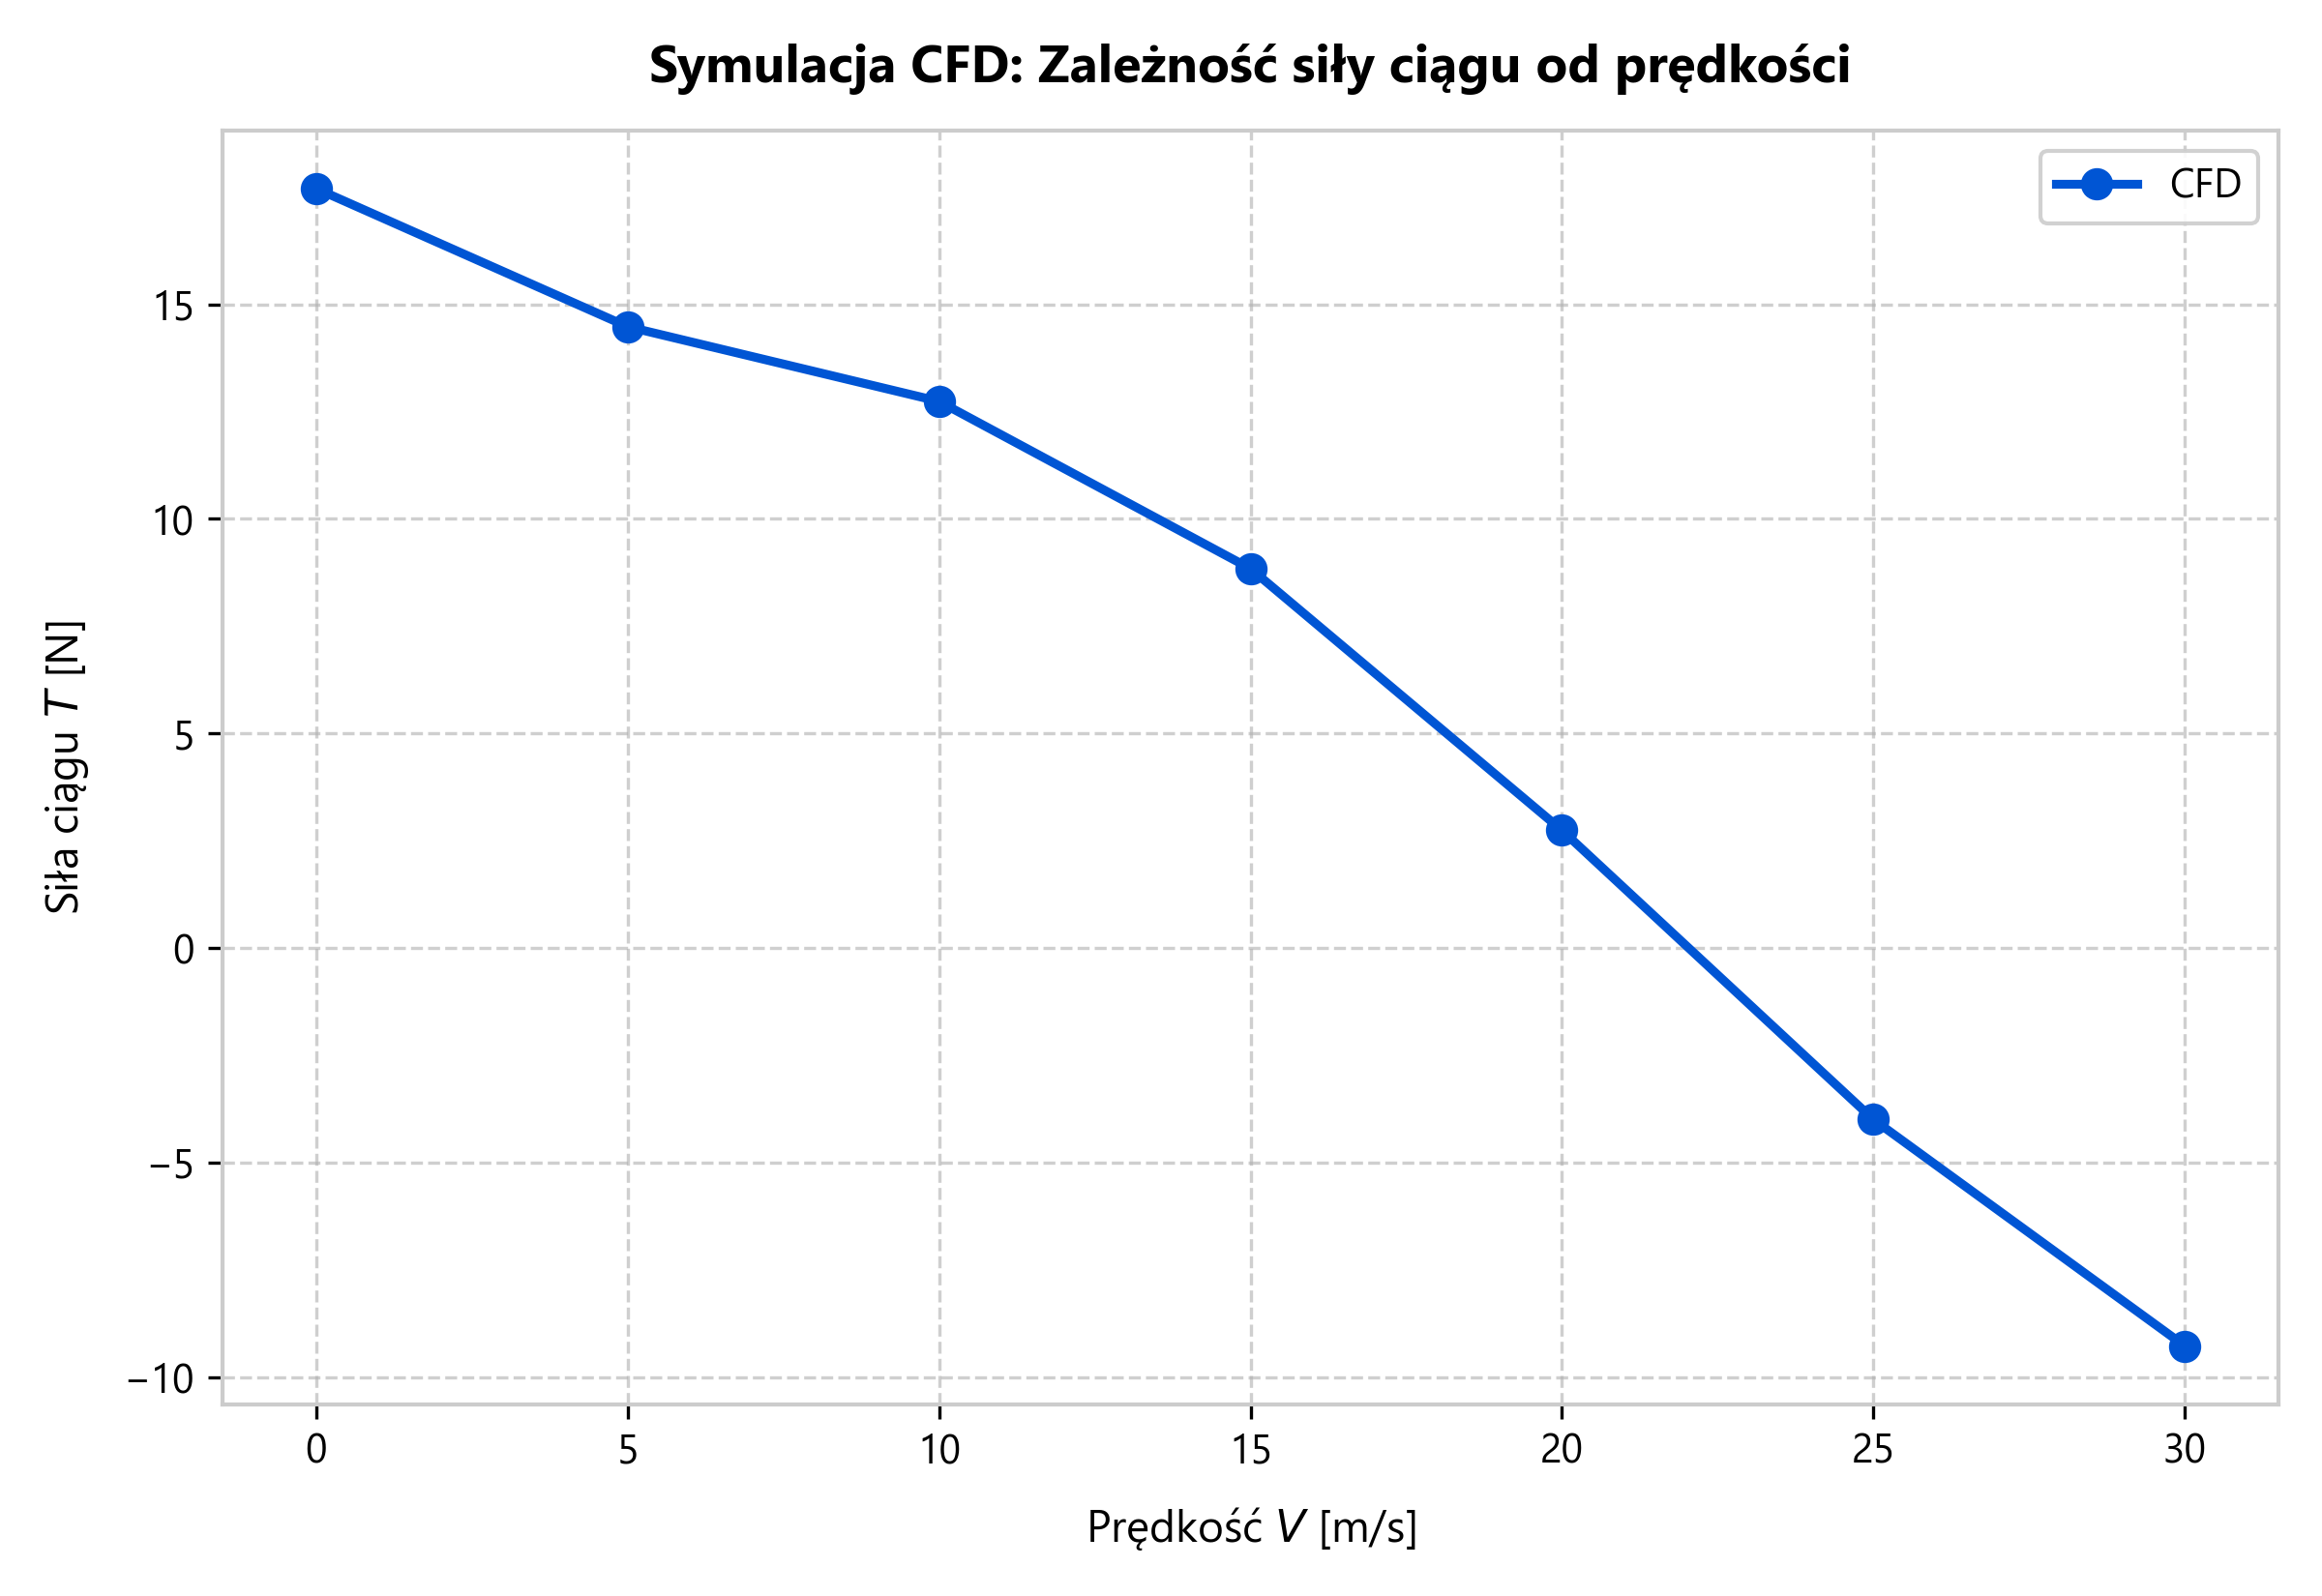
\includegraphics[width=.82\linewidth]{wykresy/01_cfd_sila_od_predkosci.png}
		\caption{Charakterystyka CFD: zależność siły ciągu \(T\) od prędkości napływu \(V\).}
		\label{fig:cfd_sila}
	\end{figure}
	
	\begin{figure}[H]\centering
		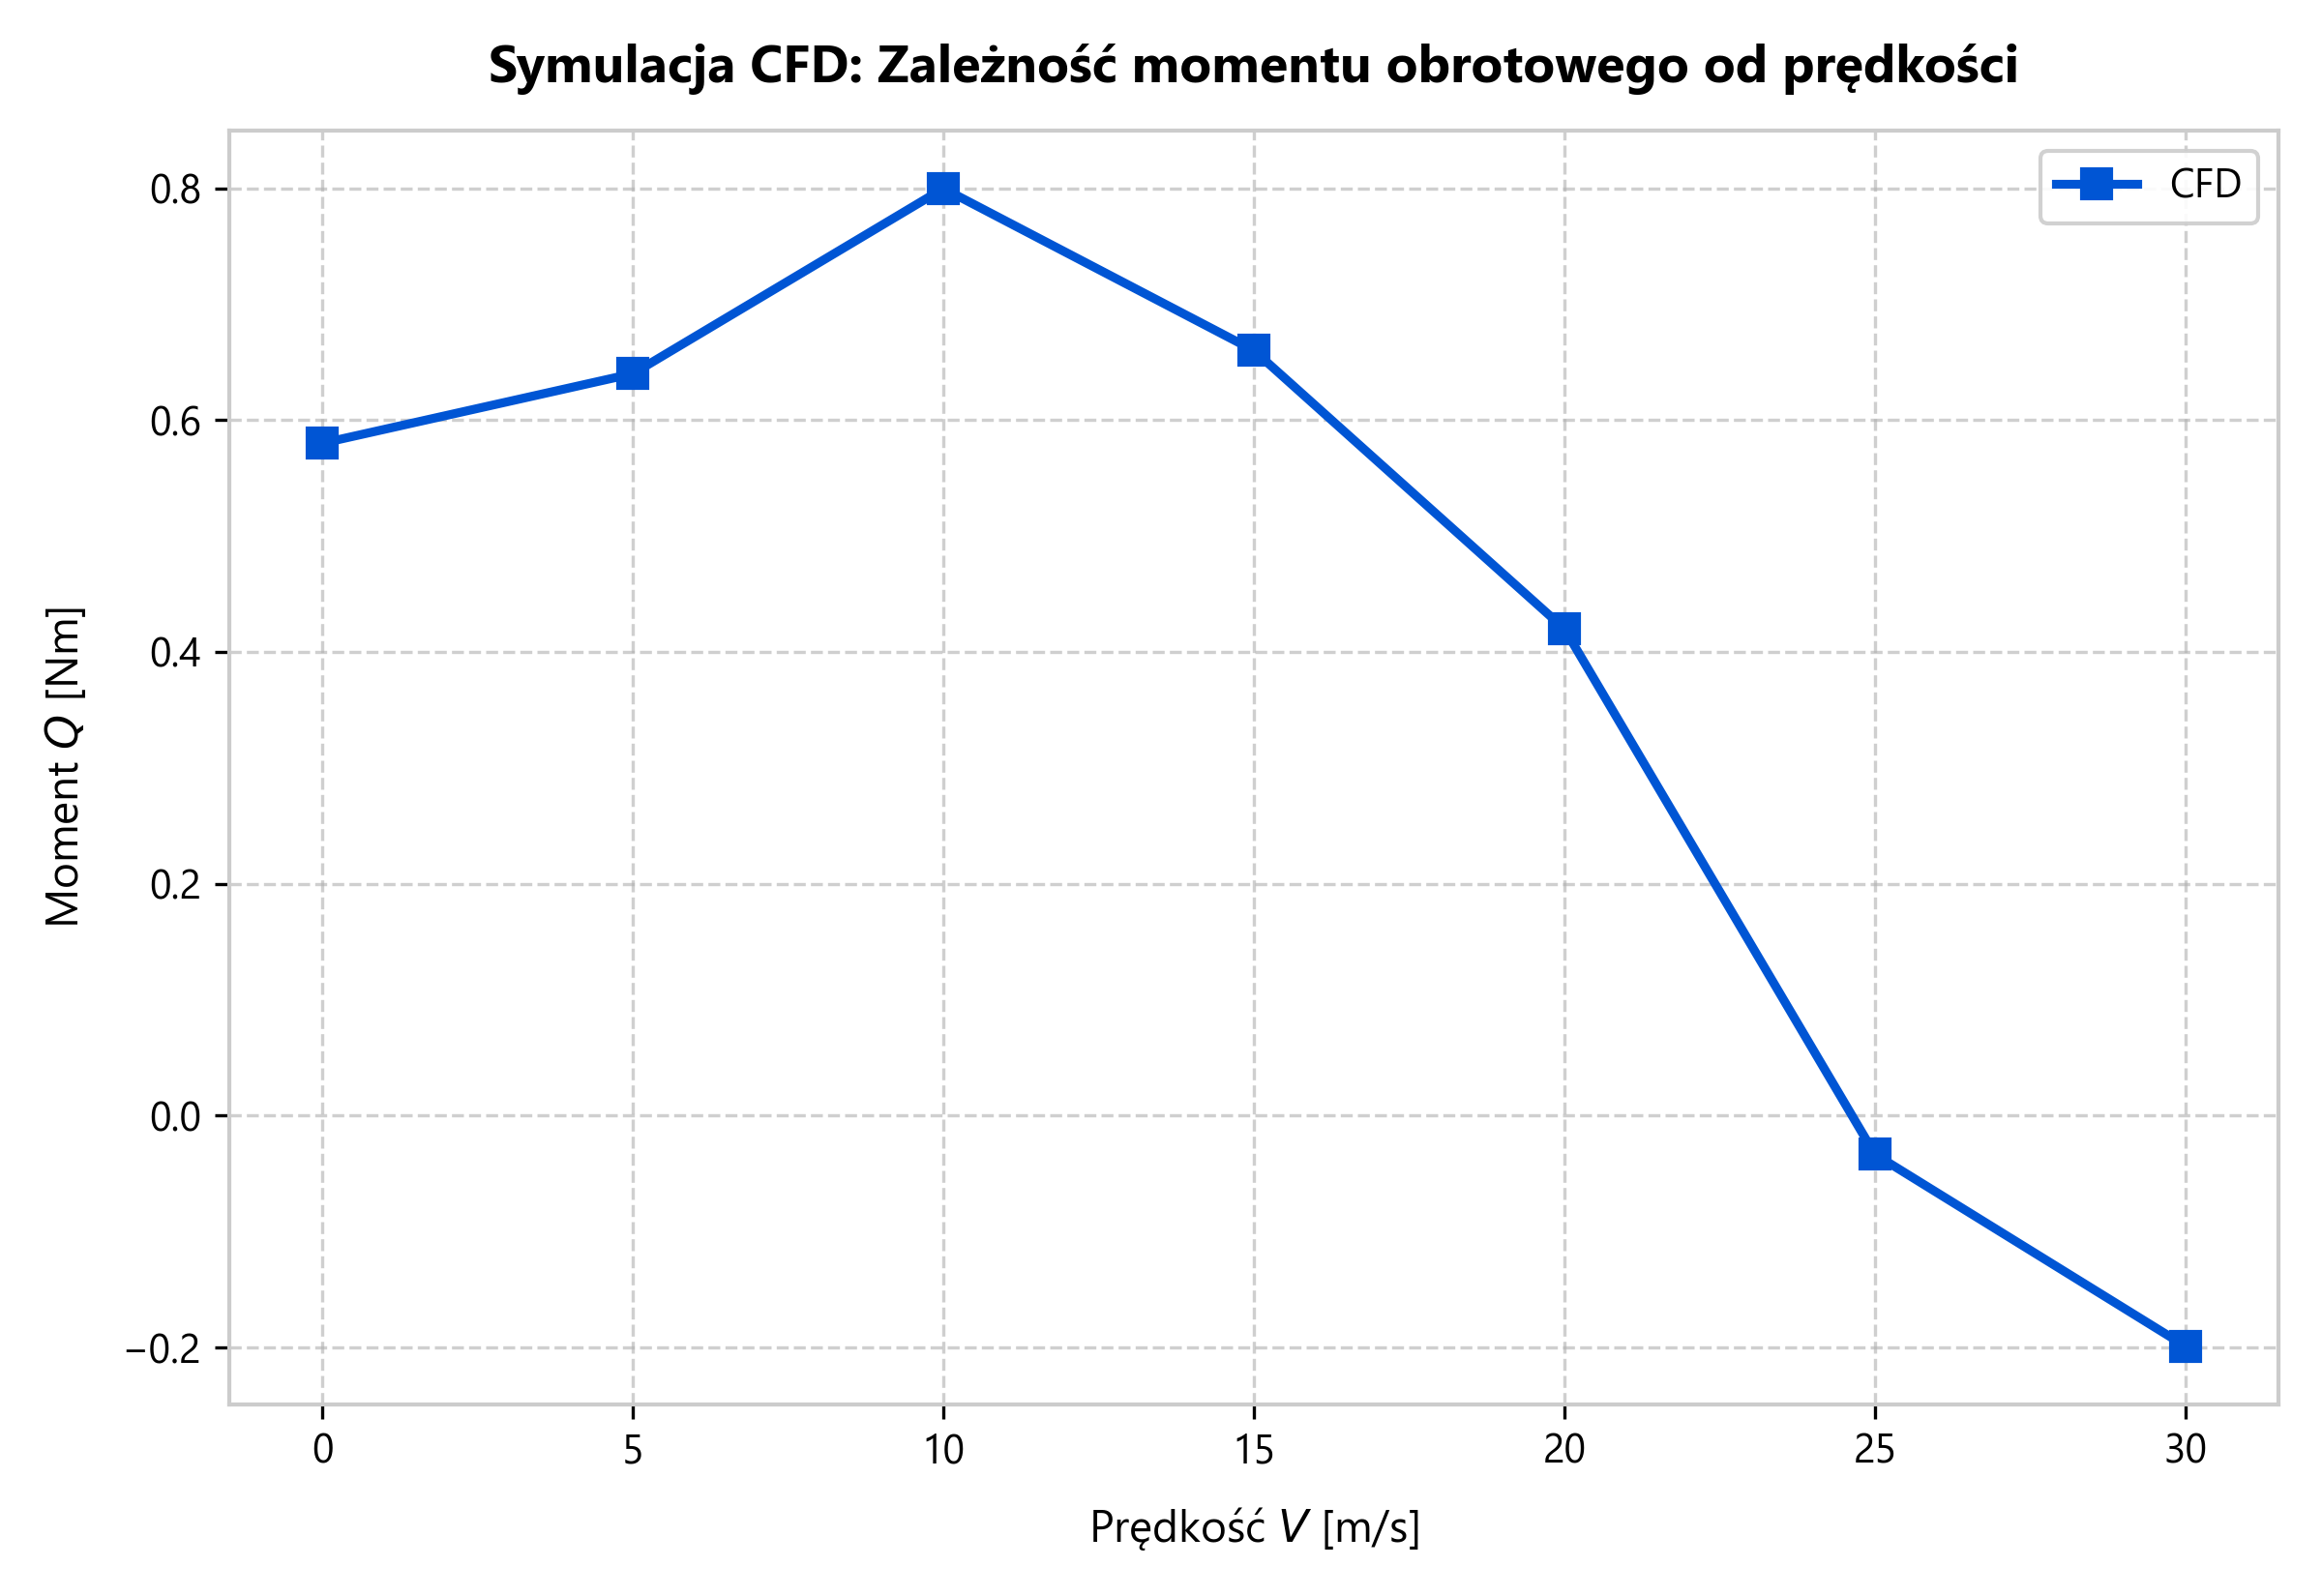
\includegraphics[width=.82\linewidth]{wykresy/02_cfd_moment_od_predkosci.png}
		\caption{Charakterystyka CFD: zależność momentu obrotowego \(Q\) od prędkości napływu \(V\).}
		\label{fig:cfd_moment}
	\end{figure}
	
	\begin{figure}[H]\centering
		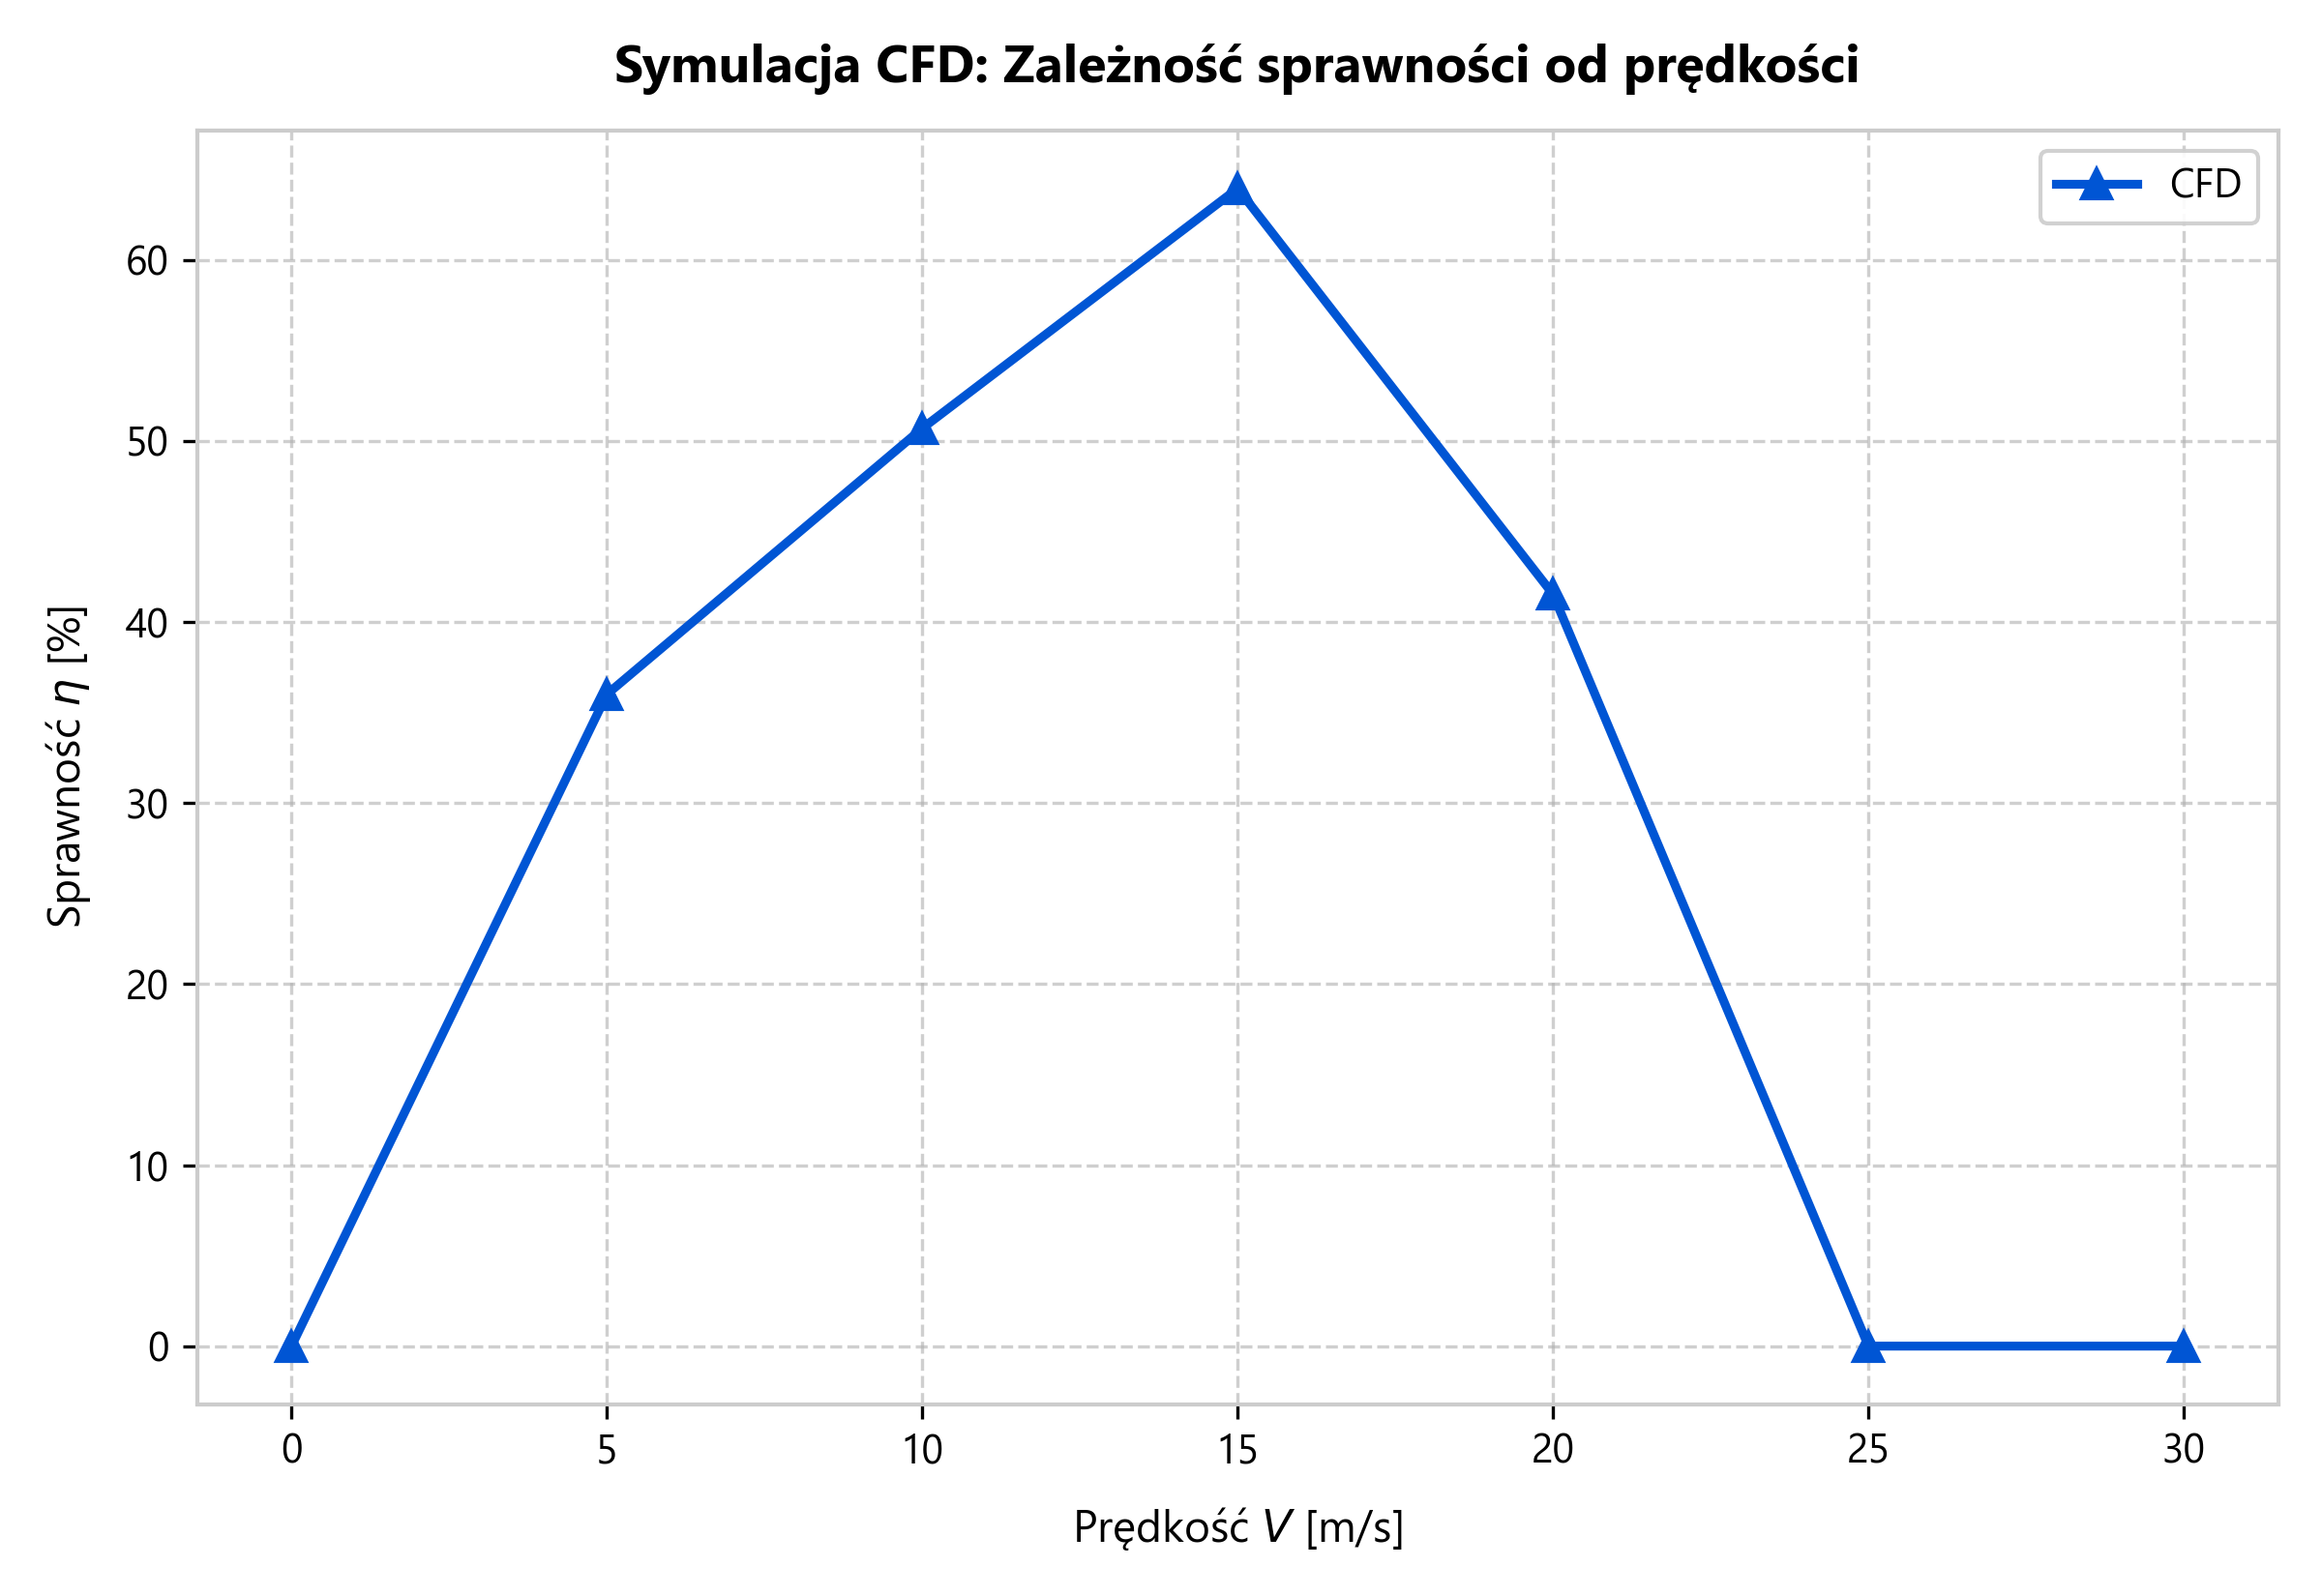
\includegraphics[width=.82\linewidth]{wykresy/03_cfd_sprawnosc_od_predkosci.png}
		\caption{Charakterystyka CFD: zależność sprawności \(\eta\) od prędkości napływu \(V\).}
		\label{fig:cfd_sprawnosc}
	\end{figure}
	
	\begin{figure}[H]\centering
		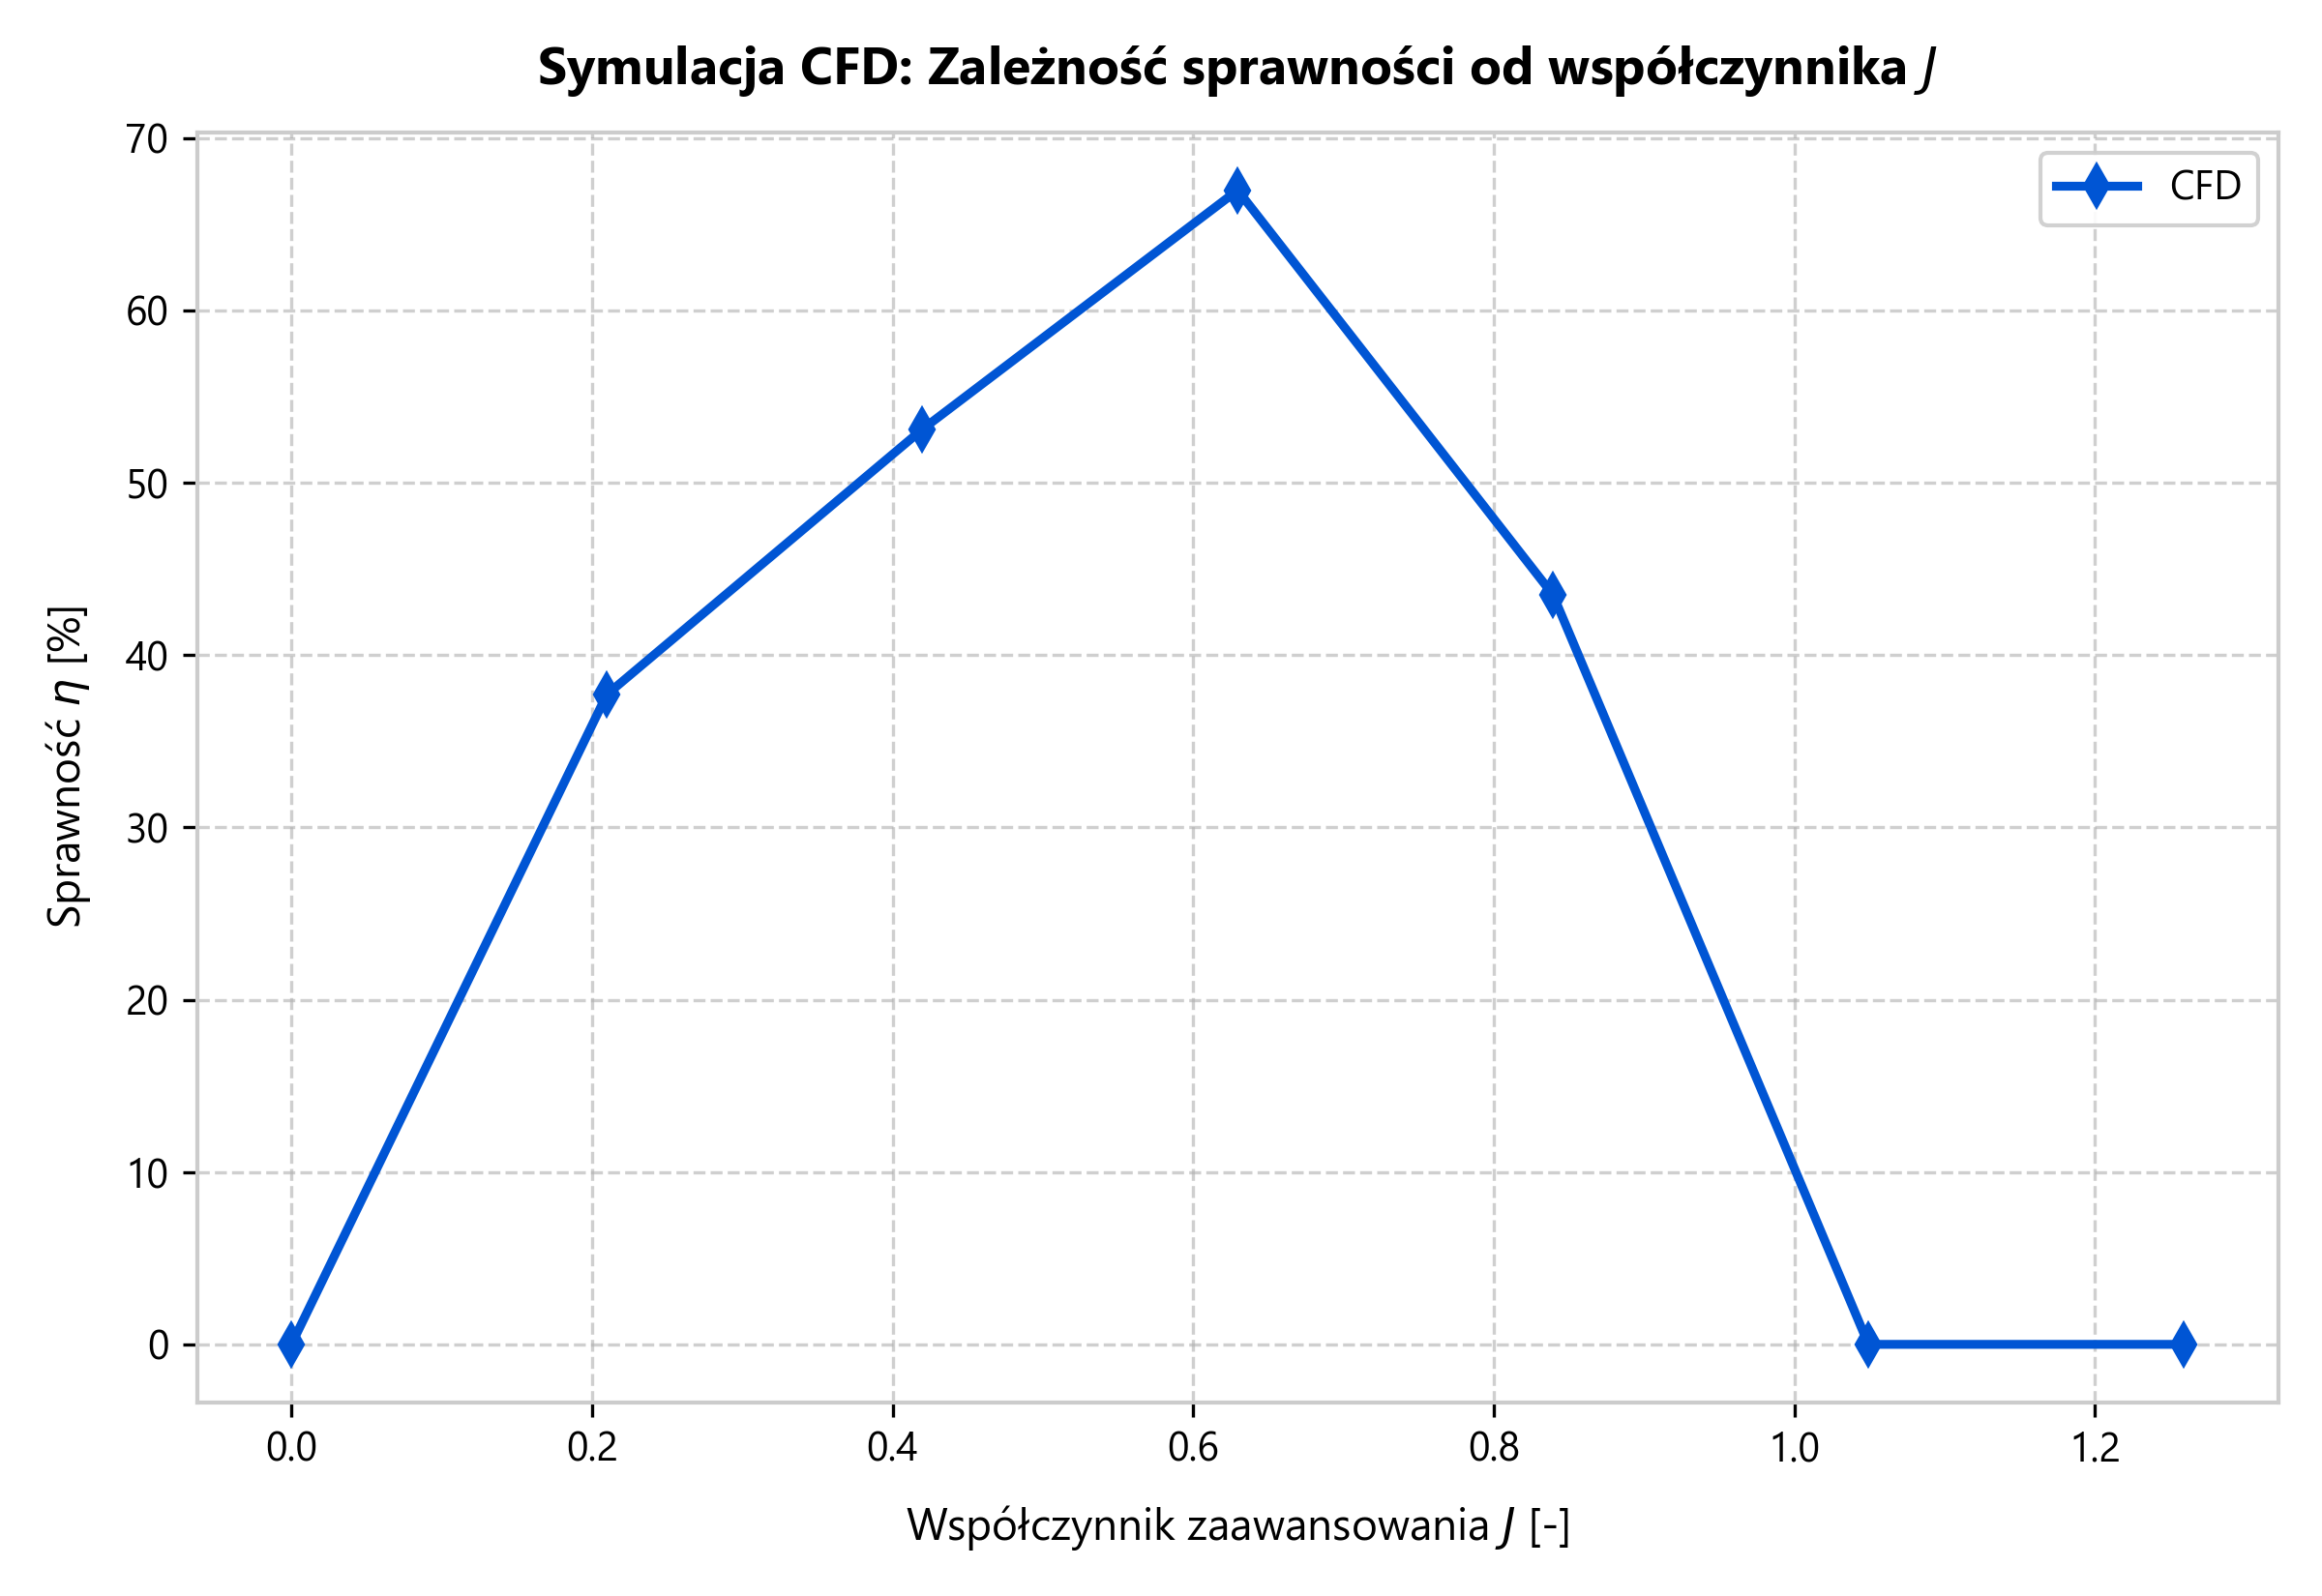
\includegraphics[width=.82\linewidth]{wykresy/04_cfd_sprawnosc_od_J.png}
		\caption{Charakterystyka CFD: zależność sprawności \(\eta\) od współczynnika zaawansowania \(J\).}
		\label{fig:cfd_sprawnosc_J}
	\end{figure}
	
	\subsubsection{Rozkłady pól przepływu wokół śmigła}
	Na rysunkach \ref{fig:vel_distrib}--\ref{fig:stat_pressure} przedstawiono graficzny rozkład pola prędkości (rys. \ref{fig:vel_distrib}), ciśnienia dynamicznego (rys. \ref{fig:dyn_pressure}) oraz ciśnienia statycznego (rys. \ref{fig:stat_pressure}) wokół śmigła dla kolejnych prędkości napływu. Rozkład prędkości pokazano dla prędkości 5--25 m/s, natomiast rozkłady ciśnień dla prędkości 10--25 m/s.
	
	\begin{figure}[H]%
		\begin{subfigure}[b]{.49\textwidth}\centering
			
\includegraphics[width=\textwidth,height=.29\textheight,keepaspectratio]{wykresy_smigla/V5/V.png}\caption{\(V_\infty = 5\) m/s.}\end{subfigure}\hfill
		\begin{subfigure}[b]{.49\textwidth}\centering
			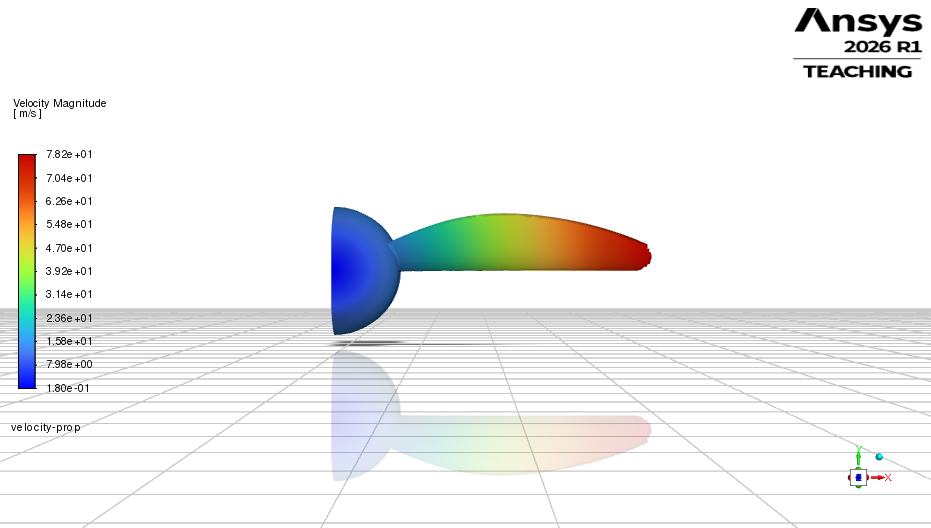
\includegraphics[width=\textwidth,height=.29\textheight,keepaspectratio]{wykresy_smigla/V10/V.png}\caption{\(V_\infty = 10\) m/s.}\end{subfigure}
		\\[.6em]
		\begin{subfigure}[b]{.49\textwidth}\centering
			
\includegraphics[width=\textwidth,height=.29\textheight,keepaspectratio]{wykresy_smigla/V15/V.png}\caption{\(V_\infty = 15\) m/s.}\end{subfigure}\hfill
		\begin{subfigure}[b]{.49\textwidth}\centering
			
\includegraphics[width=\textwidth,height=.29\textheight,keepaspectratio]{wykresy_smigla/V20/V.png}\caption{\(V_\infty = 20\) m/s.}\end{subfigure}
		\\[.6em]
		\begin{subfigure}[b]{.49\textwidth}\centering
			
\includegraphics[width=\textwidth,height=.29\textheight,keepaspectratio]{wykresy_smigla/V25/V.png}\caption{\(V_\infty = 25\) m/s.}\end{subfigure}
		\caption{Rozkład prędkości wokół śmigła dla kolejnych prędkości napływu.}
		\label{fig:vel_distrib}
	\end{figure}
	
	\begin{figure}[H]%
		\begin{subfigure}[b]{.49\textwidth}\centering
			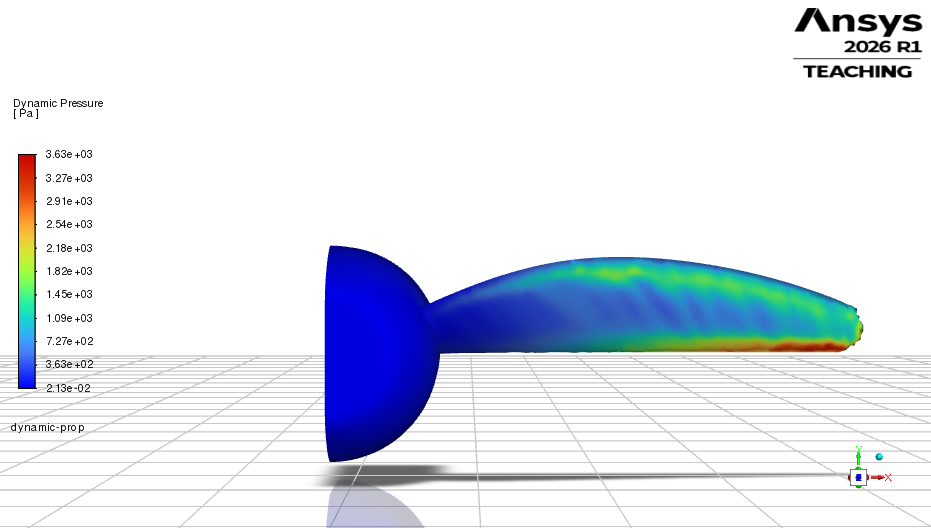
\includegraphics[width=\textwidth,height=.29\textheight,keepaspectratio]{wykresy_smigla/V10/dyn.png}\caption{\(V_\infty = 10\) m/s.}\end{subfigure}\hfill
		\begin{subfigure}[b]{.49\textwidth}\centering
			
\includegraphics[width=\textwidth,height=.29\textheight,keepaspectratio]{wykresy_smigla/V15/dyn.png}\caption{\(V_\infty = 15\) m/s.}\end{subfigure}
		\\[.6em]
		\begin{subfigure}[b]{.49\textwidth}\centering
			
\includegraphics[width=\textwidth,height=.29\textheight,keepaspectratio]{wykresy_smigla/V20/dyn.png}\caption{\(V_\infty = 20\) m/s.}\end{subfigure}\hfill
		\begin{subfigure}[b]{.49\textwidth}\centering
			
\includegraphics[width=\textwidth,height=.29\textheight,keepaspectratio]{wykresy_smigla/V25/dyn.png}\caption{\(V_\infty = 25\) m/s.}\end{subfigure}
		\caption{Rozkład ciśnienia dynamicznego wokół śmigła dla kolejnych prędkości napływu.}
		\label{fig:dyn_pressure}
	\end{figure}
	
	\begin{figure}[H]%
		\begin{subfigure}[b]{.49\textwidth}\centering
			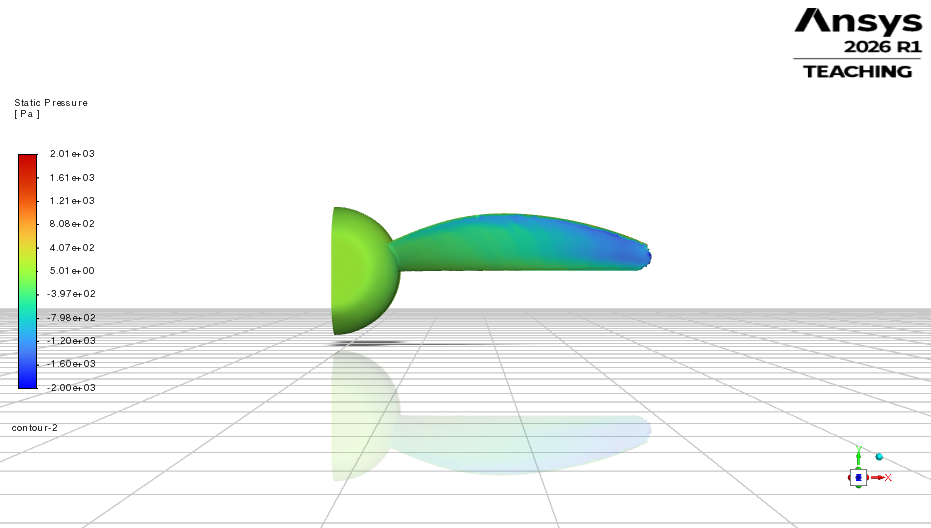
\includegraphics[width=\textwidth,height=.29\textheight,keepaspectratio]{wykresy_smigla/V10/stat.png}\caption{\(V_\infty = 10\) m/s.}\end{subfigure}\hfill
		\begin{subfigure}[b]{.49\textwidth}\centering
			
\includegraphics[width=\textwidth,height=.29\textheight,keepaspectratio]{wykresy_smigla/V15/stat.png}\caption{\(V_\infty = 15\) m/s.}\end{subfigure}
		\\[.6em]
		\begin{subfigure}[b]{.49\textwidth}\centering
			
\includegraphics[width=\textwidth,height=.29\textheight,keepaspectratio]{wykresy_smigla/V20/stat.png}\caption{\(V_\infty = 20\) m/s.}\end{subfigure}\hfill
		\begin{subfigure}[b]{.49\textwidth}\centering
			
\includegraphics[width=\textwidth,height=.29\textheight,keepaspectratio]{wykresy_smigla/V25/stat.png}\caption{\(V_\infty = 25\) m/s.}\end{subfigure}
		\caption{Rozkład ciśnienia statycznego wokół śmigła dla kolejnych prędkości napływu.}
		\label{fig:stat_pressure}
	\end{figure}
	
	\subsection{Walidacja wyników CFD z metodą BEMT}
	
	\subsubsection{Zestawienie porównawcze}
	W tabeli \ref{tab:comparison} zestawiono wyniki metody BMT oraz symulacji CFD dla ciągu i momentu obrotowego wraz z błędem względnym liczonym względem wartości referencyjnej BMT. Ujemne wartości błędu oznaczają, że wynik CFD jest niższy od wyniku BMT, dodatnie -- że jest wyższy. Tabela \ref{tab:errors_comparison} zawiera błędy względne mocy i sprawności.
	
	\begin{table}[H]
		\centering
		\small
		\caption{Porównanie wyników BMT i CFD oraz błędy względne dla ciągu \(T\) i momentu obrotowego \(Q\).}
		\label{tab:comparison}
		\begin{tabular}{@{}c c c c c c c@{}}
			\toprule
			\(V_\infty\) & \(T_{\text{BMT}}\) & \(T_{\text{CFD}}\) & \(\delta T\) & \(Q_{\text{BMT}}\) & \(Q_{\text{CFD}}\) & \(\delta Q\) \\
 			{[m/s]} & {[N]} & {[N]} & {[\%]} & {[Nm]} & {[Nm]} & {[\%]} \\
			\midrule
			0  & 27,260  & 19,080  & -30,0  & 0,906  & 0,580  & -36,0 \\
			5  & 25,364  & 14,480  & -42,9  & 1,037  & 0,640  & -38,3 \\
			10 & 21,394  & 12,739  & -40,5  & 1,072  & 0,800  & -25,4 \\
			15 & 15,105  & 8,840   & -41,5  & 0,919  & 0,660  & -28,2 \\
			20 & 7,487   & 2,740   & -63,4  & 0,568  & 0,420  & -26,1 \\
			25 & -1,505  & -4,001  & -165,9 & -0,035 & -0,033 & +4,8  \\
			30 & -9,935  & -9,280  & +6,6   & -0,697 & -0,199 & +71,5 \\
			\bottomrule
		\end{tabular}
	\end{table}
	
	\begin{table}[H]
		\centering
		\small
		\caption{Błędy względne metody CFD względem BMT dla mocy \(P\), ciągu \(T\), momentu \(Q\) i sprawności \(\eta\).}
		\label{tab:errors_comparison}
		\begin{tabular}{@{}c c c c c@{}}
			\toprule
			\(V_\infty\) & \(\delta P\) & \(\delta T\) & \(\delta Q\) & \(\delta\eta\) \\
			{[m/s]} & {[\%]} & {[\%]} & {[\%]} & {[\%]} \\
			\midrule
			0  & -38,9  & -30,0  & -36,0  & 0,0   \\
			5  & -41,1  & -42,9  & -38,3  & -3,1  \\
			10 & -28,7  & -40,5  & -25,4  & -16,5 \\
			15 & -31,4  & -41,5  & -28,2  & -14,7 \\
			20 & -29,4  & -63,4  & -26,1  & -48,2 \\
			25 & +9,6   & -165,9 & +4,8   & 0,0   \\
			30 & +72,8  & +6,6   & +71,5  & 0,0   \\
			\bottomrule
		\end{tabular}
	\end{table}
	
	Największe względne rozbieżności ciągu dotyczą obszaru zmiany znaku wielkości otaczającego \(V_\infty = 25\) m/s oraz małych wartości bezwzględnych, dla których nawet niewielka różnica bezwzględna daje dużą różnicę względną. W zakresie pracy hamulcowej (\(V_\infty = 30\) m/s) błąd względny ciągu spada do ok. \(+6{,}6\%\). Bezwzględne rozbieżności momentu obrotowego są największe przy \(V_\infty = 30\) m/s (+71,5\%), gdzie obie metody przewidują niewielkie wartości ujemne.
	
	\subsubsection{Wykresy porównawcze}
	Na rysunkach \ref{fig:por_sprawnosc}--\ref{fig:por_moment} zestawiono krzywe sprawności, siły ciągu i momentu obrotowego uzyskane metodą CFD oraz metodą BMT.
	
	\begin{figure}[H]\centering
		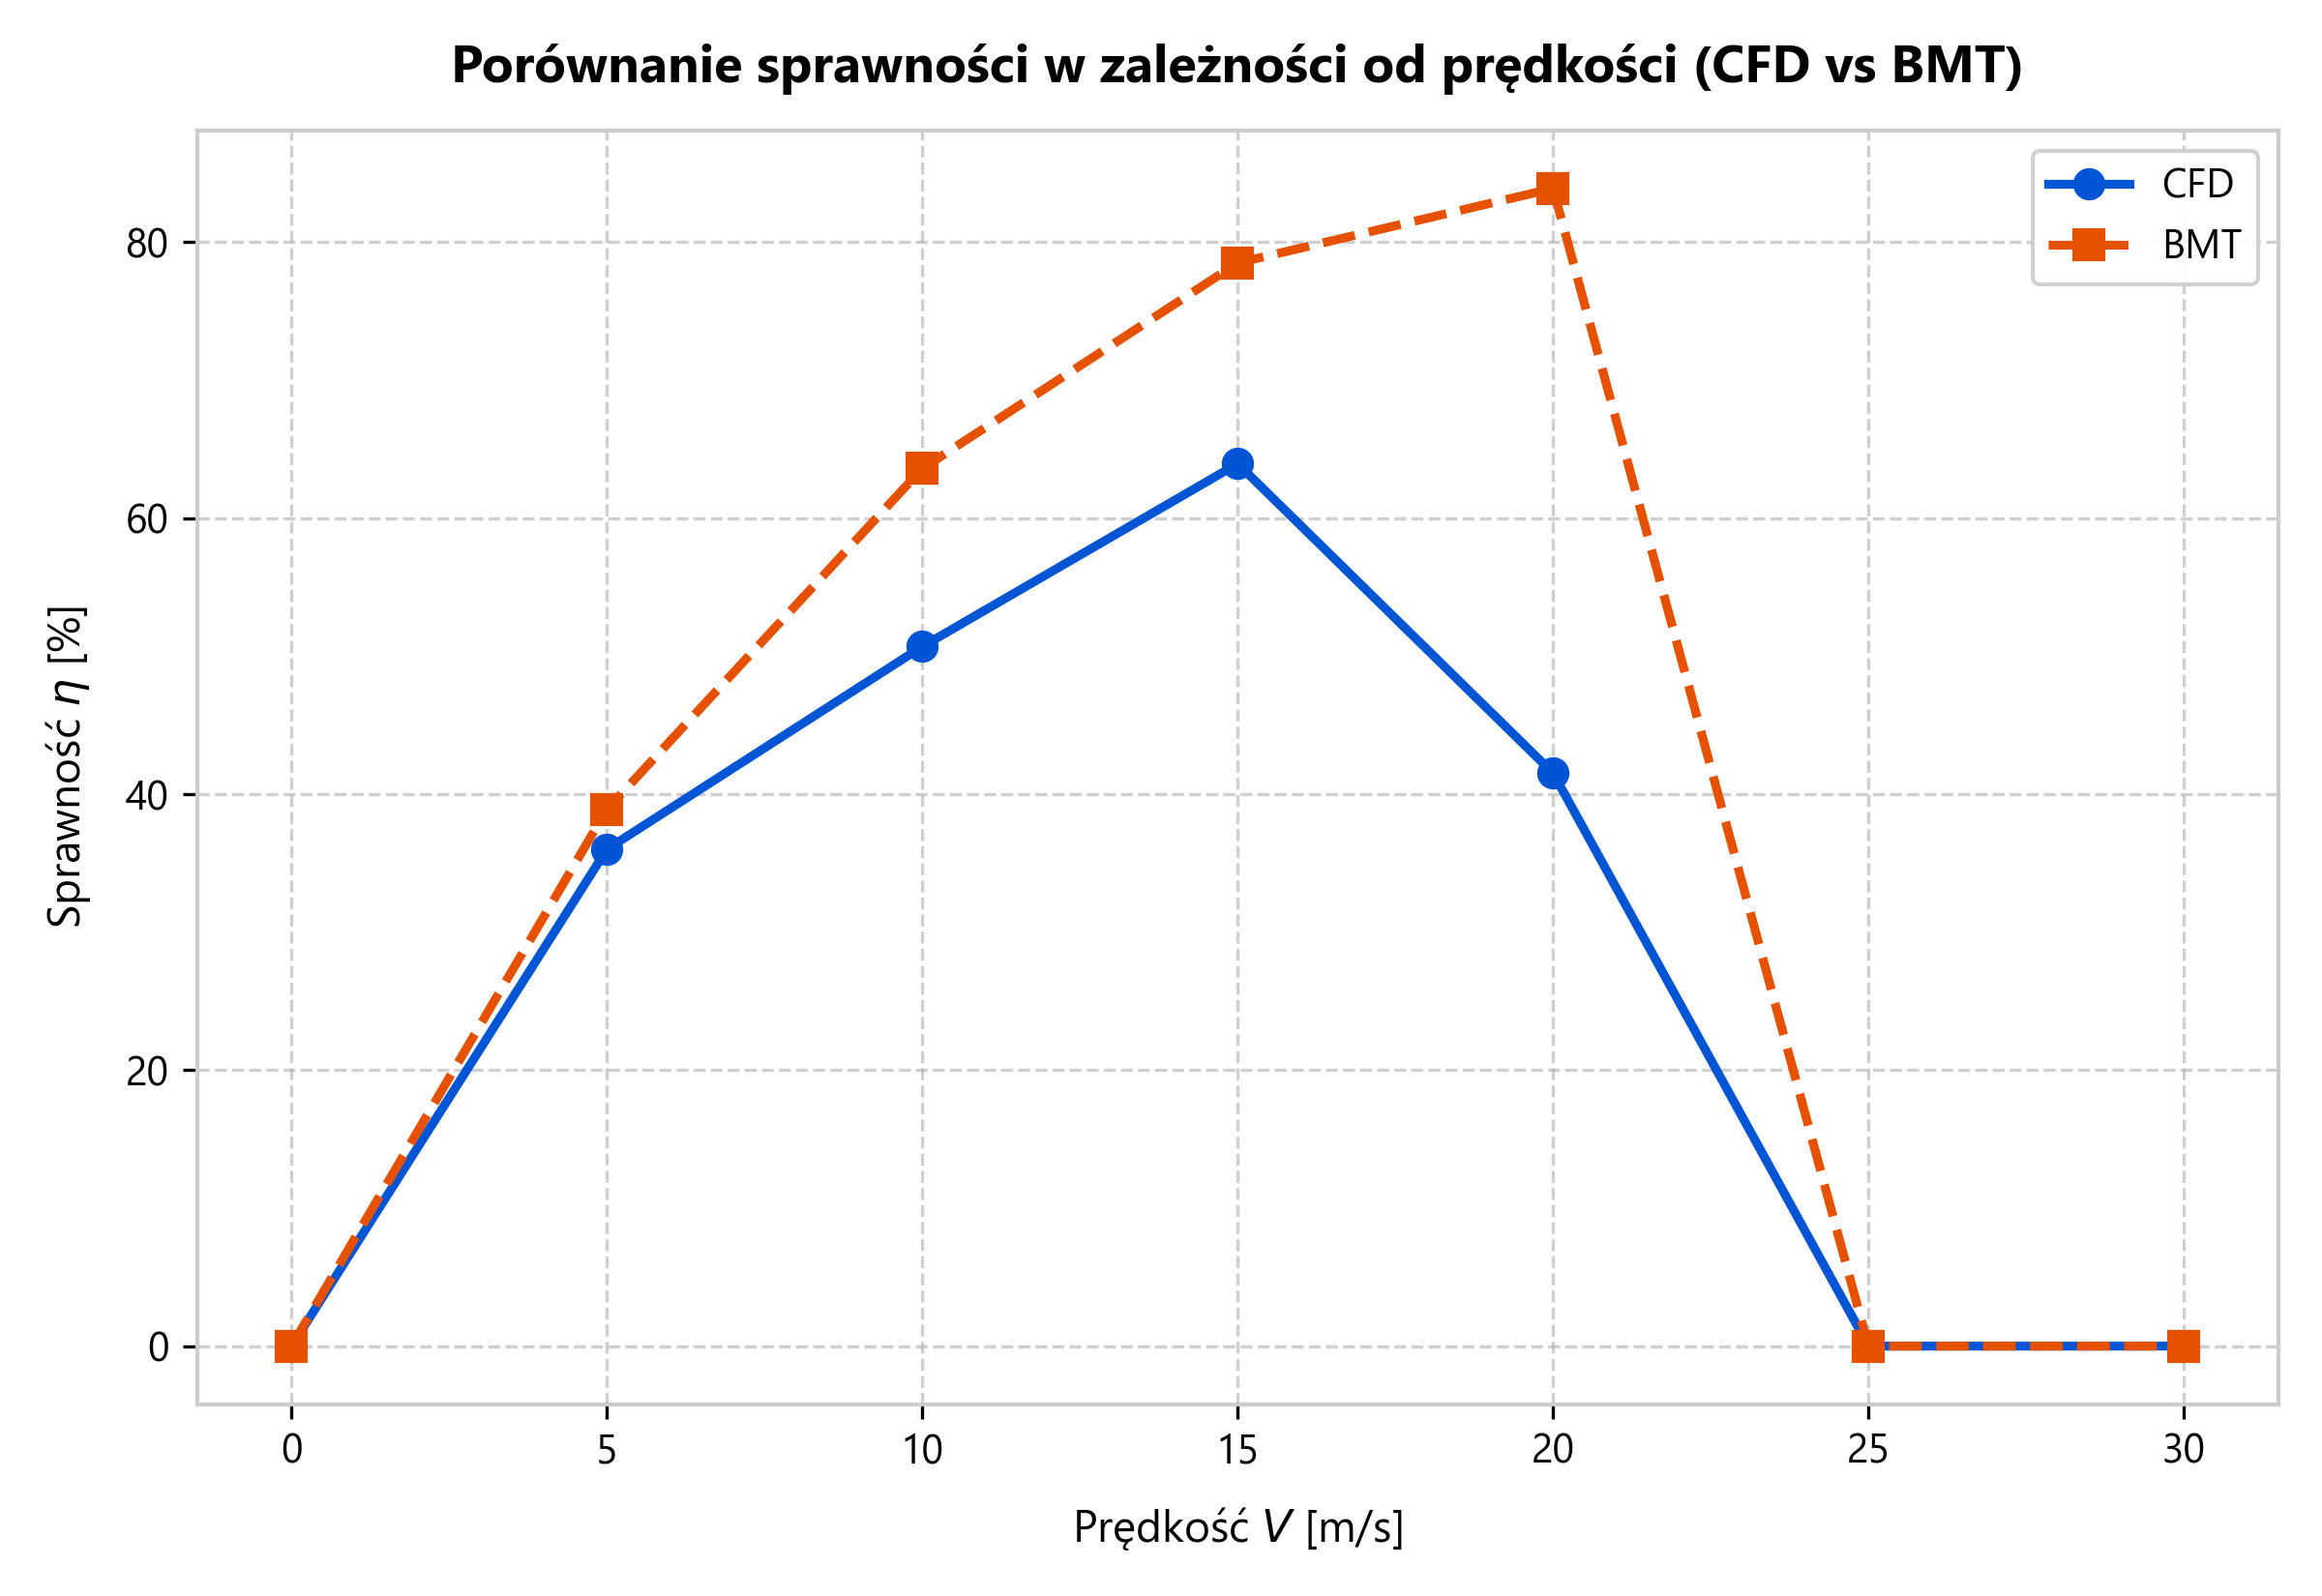
\includegraphics[width=.82\linewidth]{wykresy/05_porownanie_sprawnosc_od_predkosci.png}
		\caption{Porównanie sprawności \(\eta\) wyznaczonej metodą CFD i BMT w funkcji prędkości napływu \(V\).}
		\label{fig:por_sprawnosc}
	\end{figure}
	
	\begin{figure}[H]\centering
		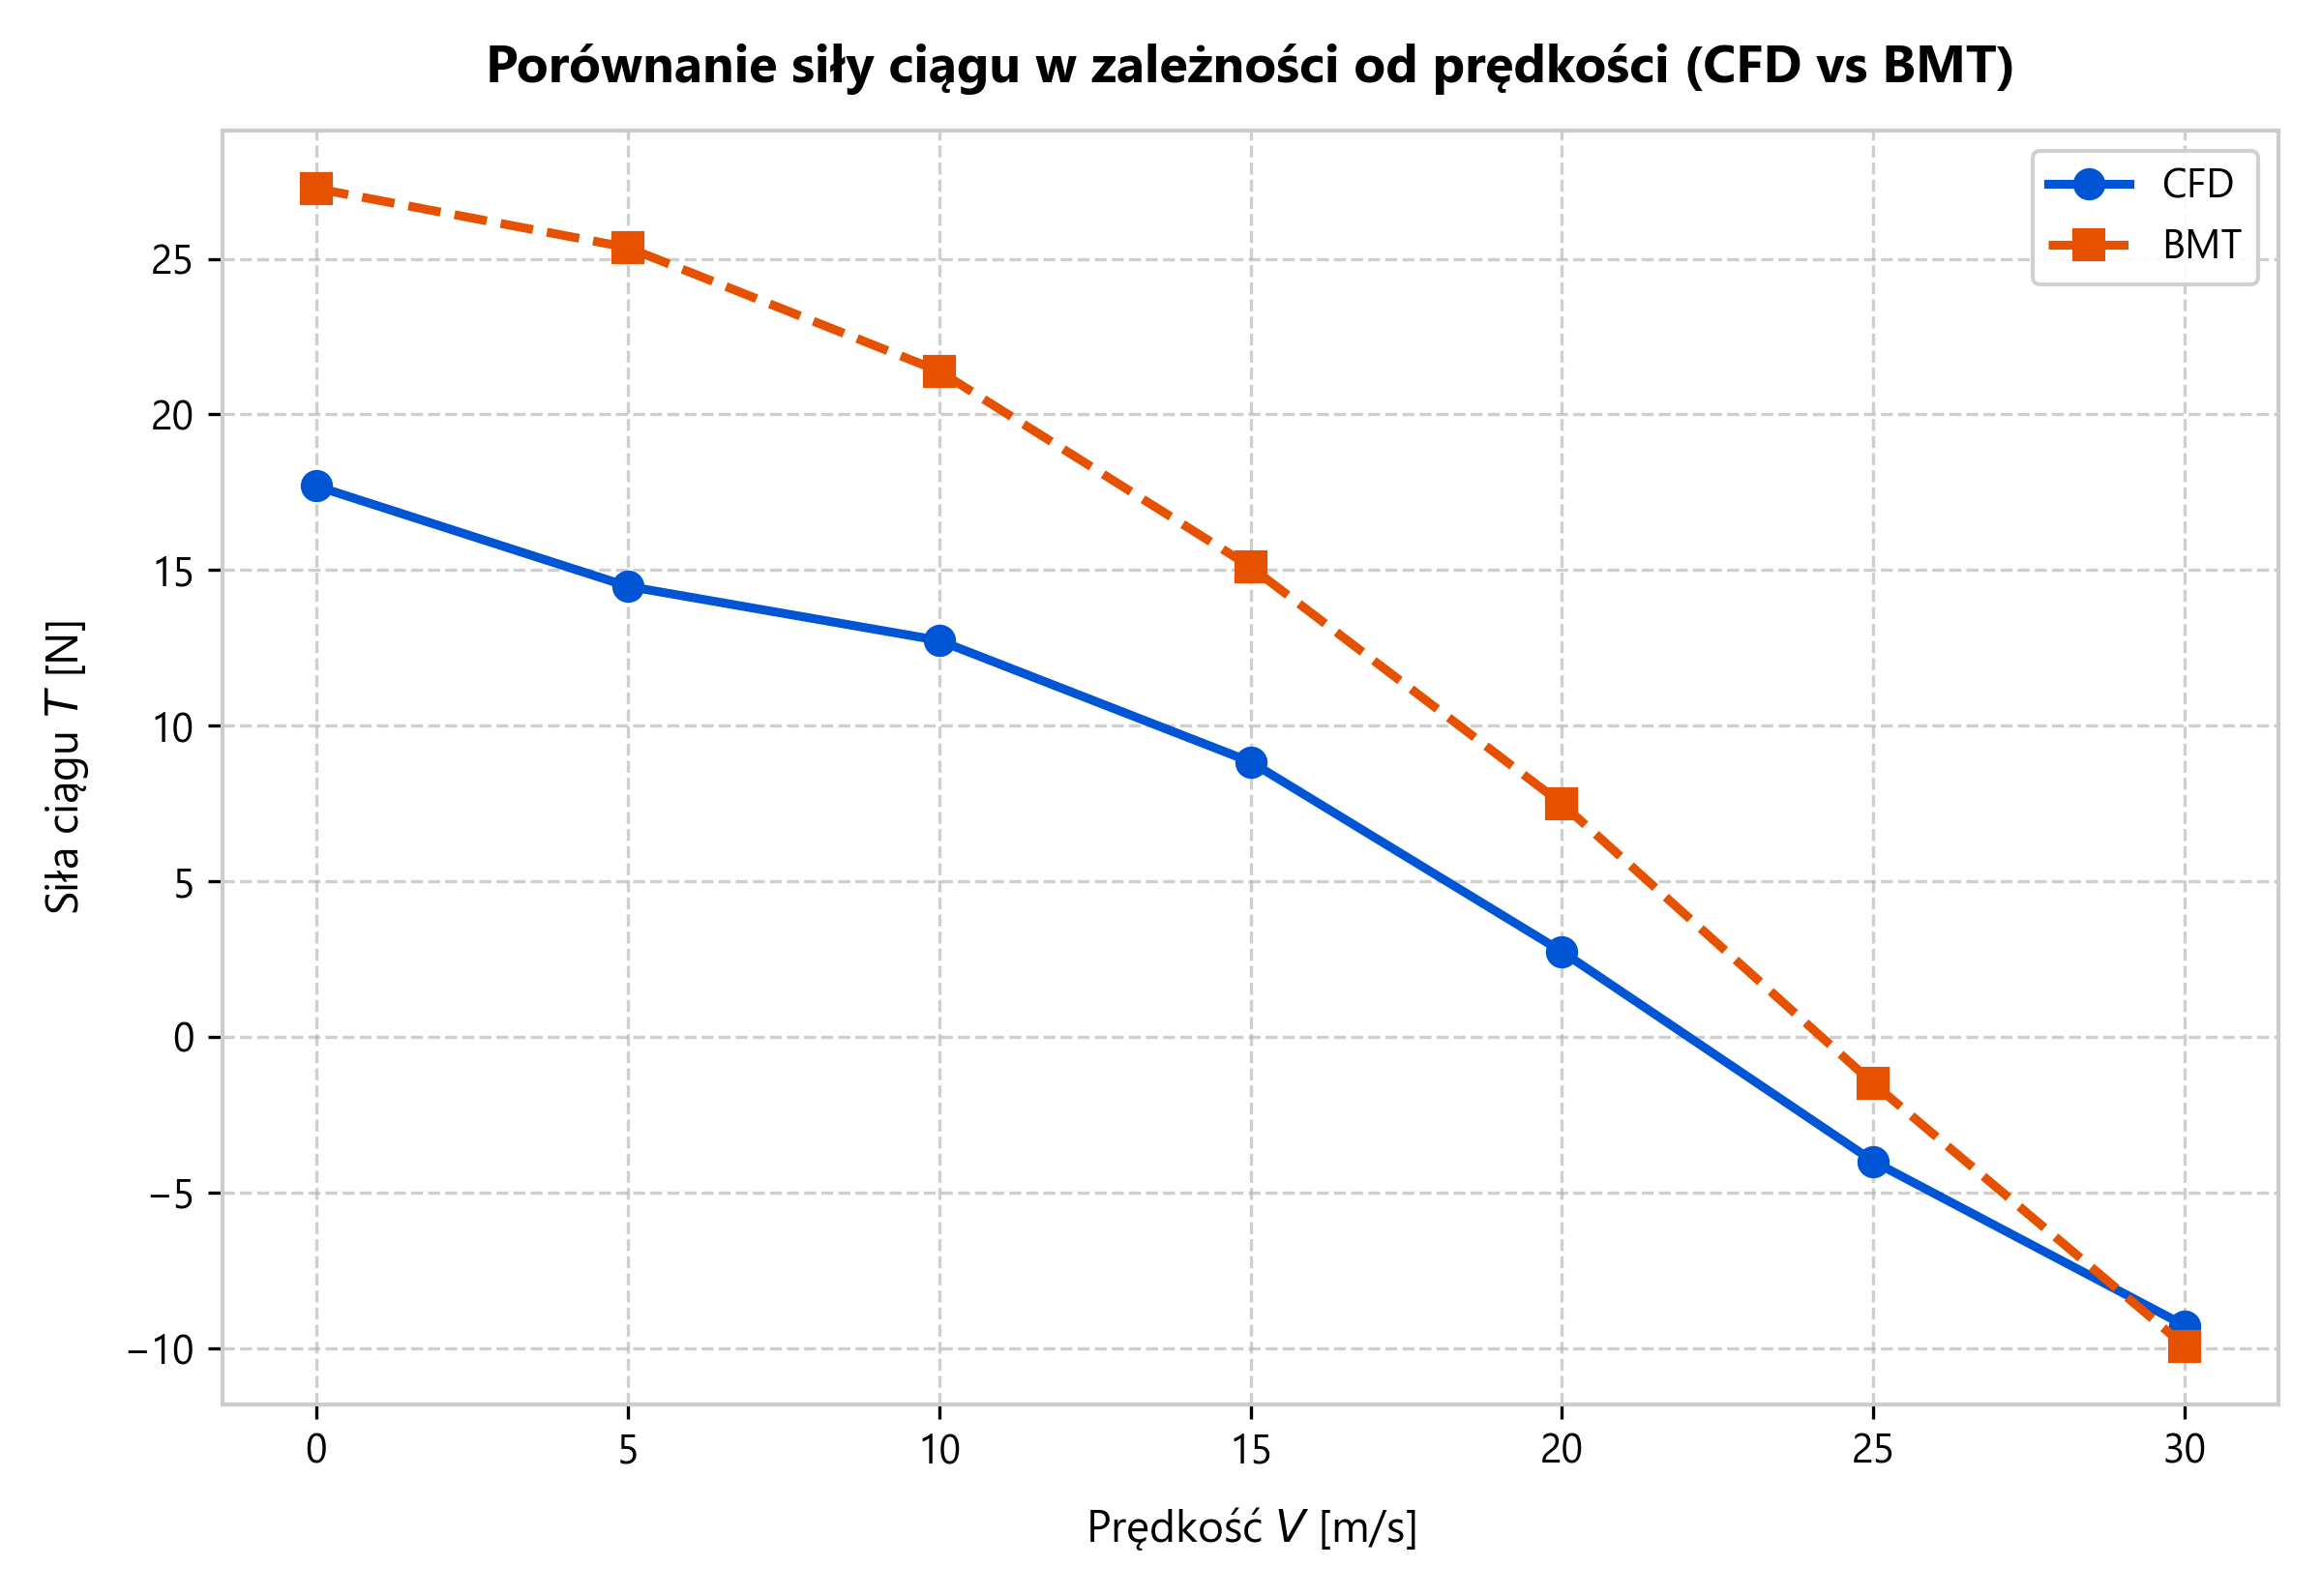
\includegraphics[width=.82\linewidth]{wykresy/06_porownanie_sila_od_predkosci.png}
		\caption{Porównanie siły ciągu \(T\) wyznaczonej metodą CFD i BMT w funkcji prędkości napływu \(V\).}
		\label{fig:por_sila}
	\end{figure}
	
	\begin{figure}[H]\centering
		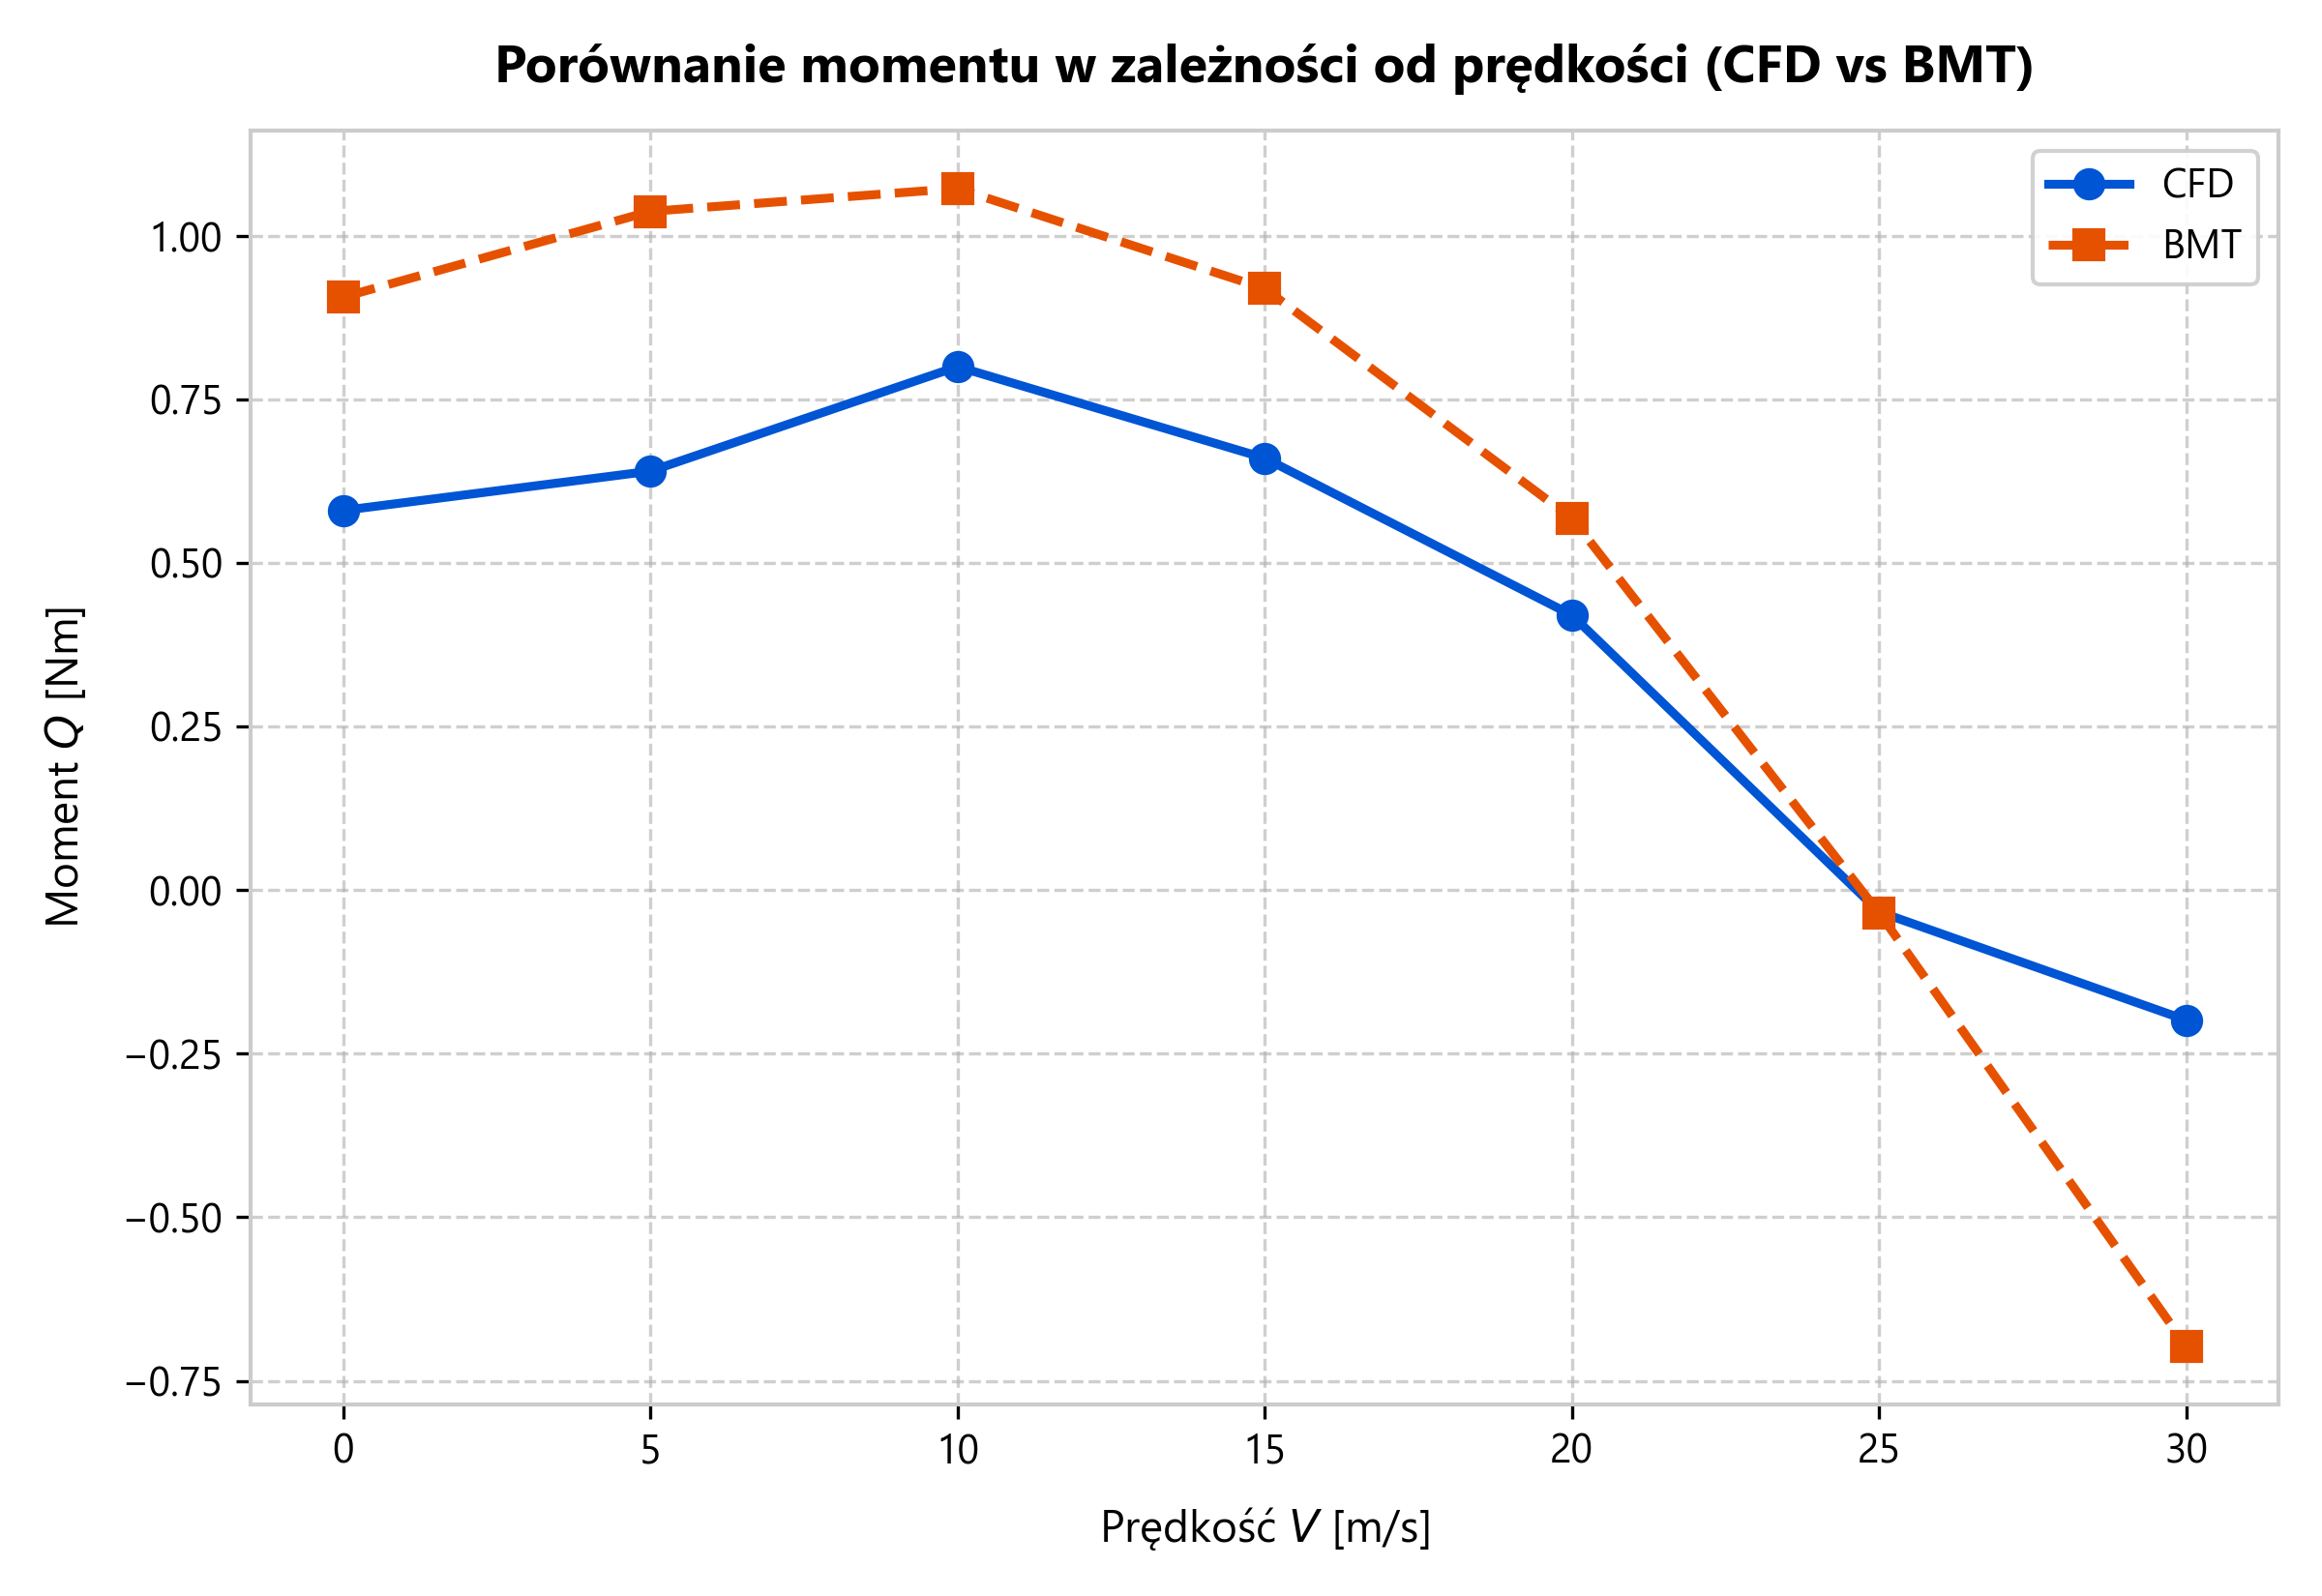
\includegraphics[width=.82\linewidth]{wykresy/07_porownanie_moment_od_predkosci.png}
		\caption{Porównanie momentu obrotowego \(Q\) wyznaczonego metodą CFD i BMT w funkcji prędkości napływu \(V\).}
		\label{fig:por_moment}
	\end{figure}
	
	\subsubsection{Wykresy błędów względnych}
	Na rysunkach \ref{fig:blad_moc}--\ref{fig:blad_sprawnosc} przedstawiono błędy względne mocy, siły ciągu i sprawności metody CFD względem metody BMT, z naniesionymi wartościami na punkty pomiarowe.
	
	\begin{figure}[H]\centering
		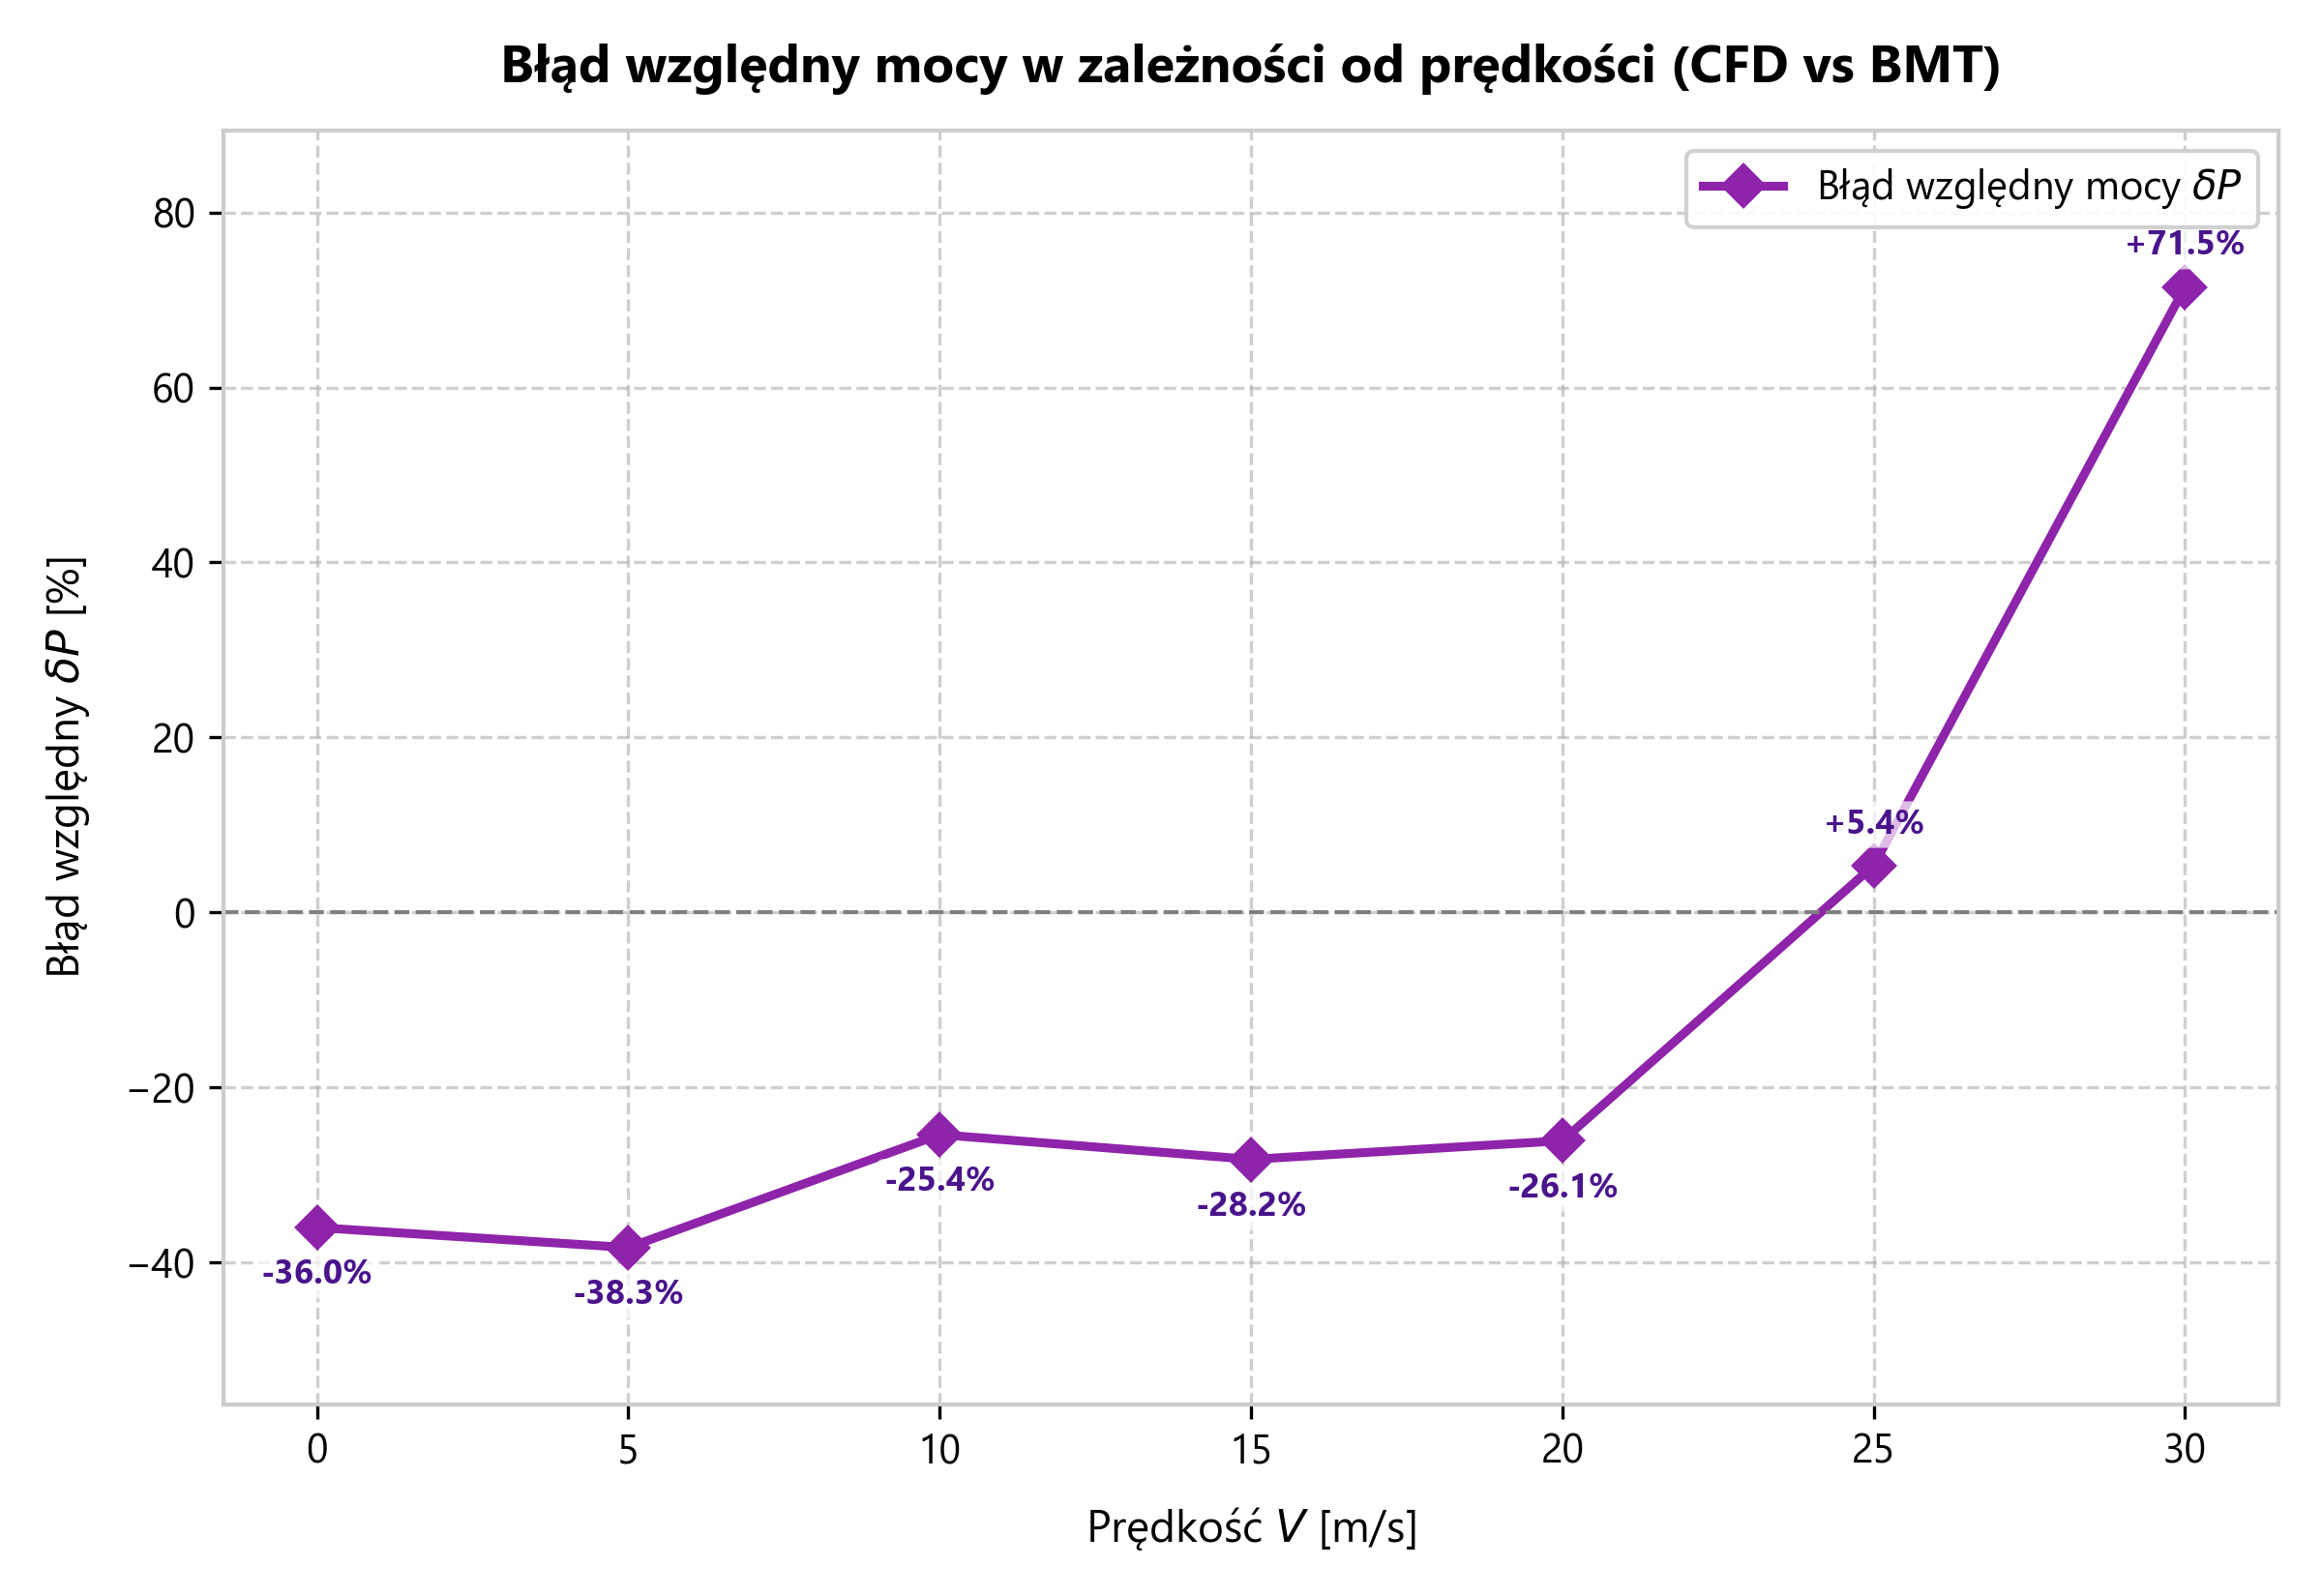
\includegraphics[width=.82\linewidth]{wykresy/08_blad_wzgledny_moc.png}
		\caption{Błąd względny mocy \(\delta P\) w funkcji prędkości napływu \(V\).}
		\label{fig:blad_moc}
	\end{figure}
	
	\begin{figure}[H]\centering
		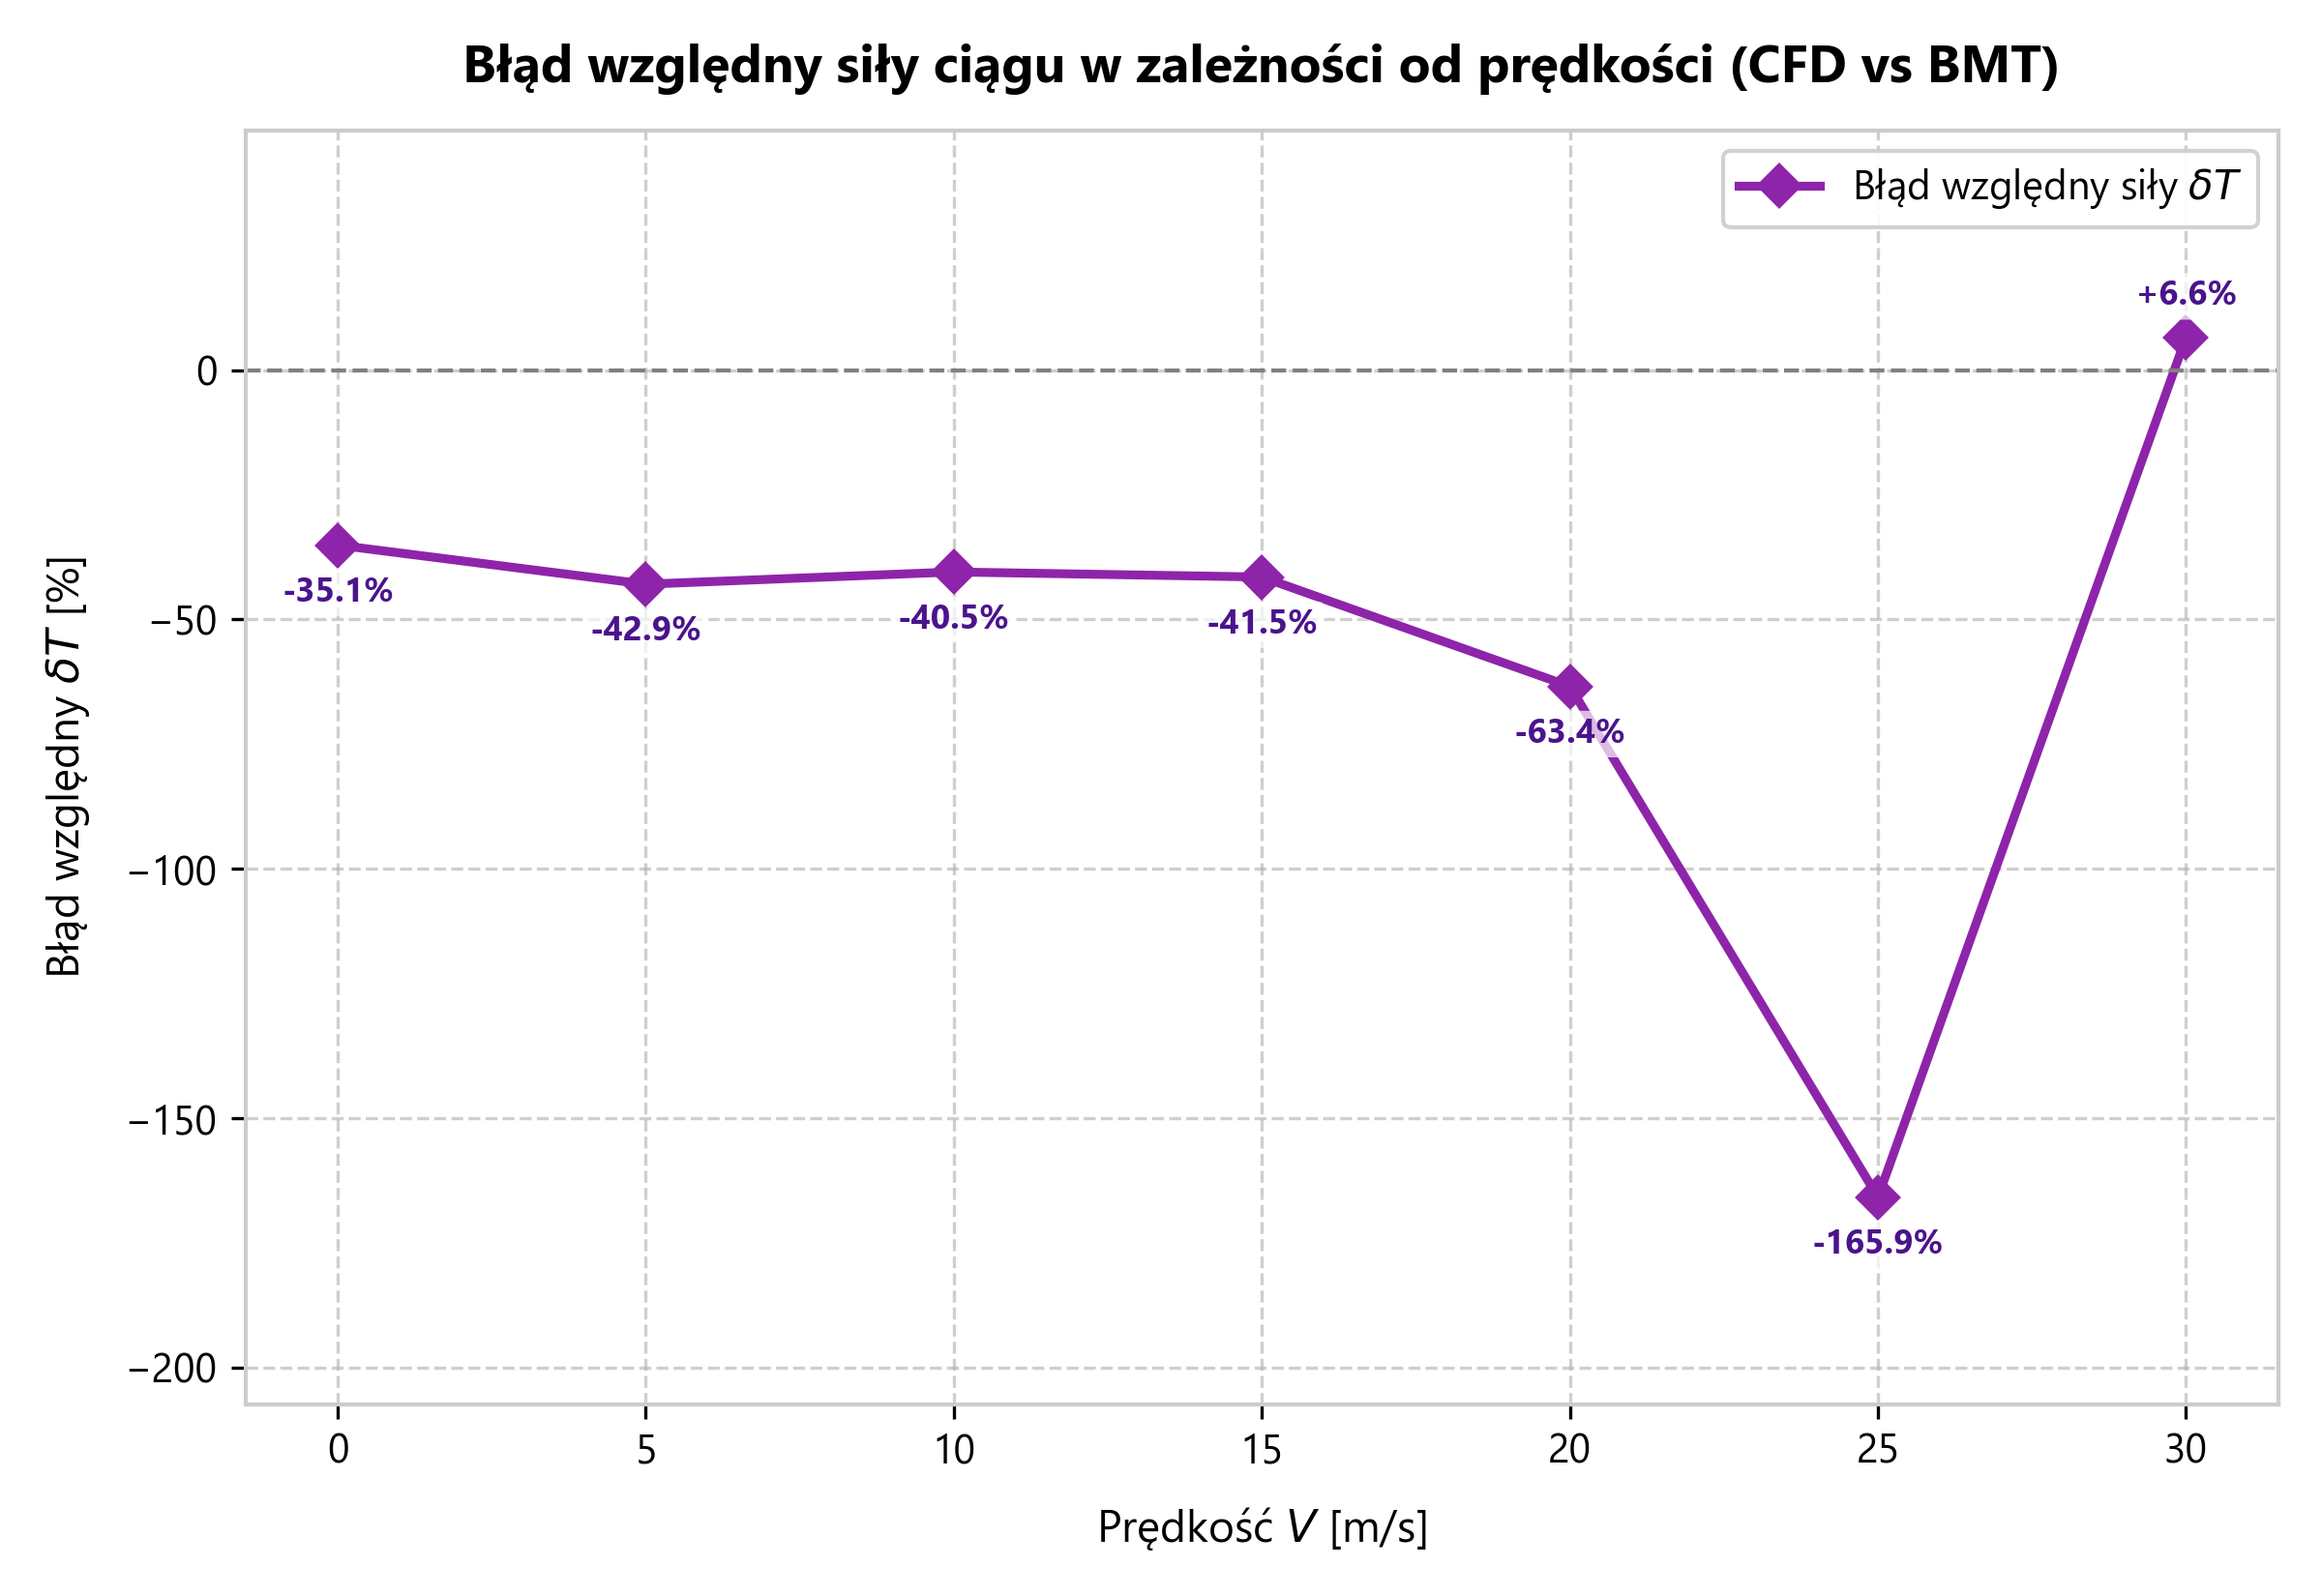
\includegraphics[width=.82\linewidth]{wykresy/09_blad_wzgledny_sila.png}
		\caption{Błąd względny siły ciągu \(\delta T\) w funkcji prędkości napływu \(V\).}
		\label{fig:blad_sila}
	\end{figure}
	
	\begin{figure}[H]\centering
		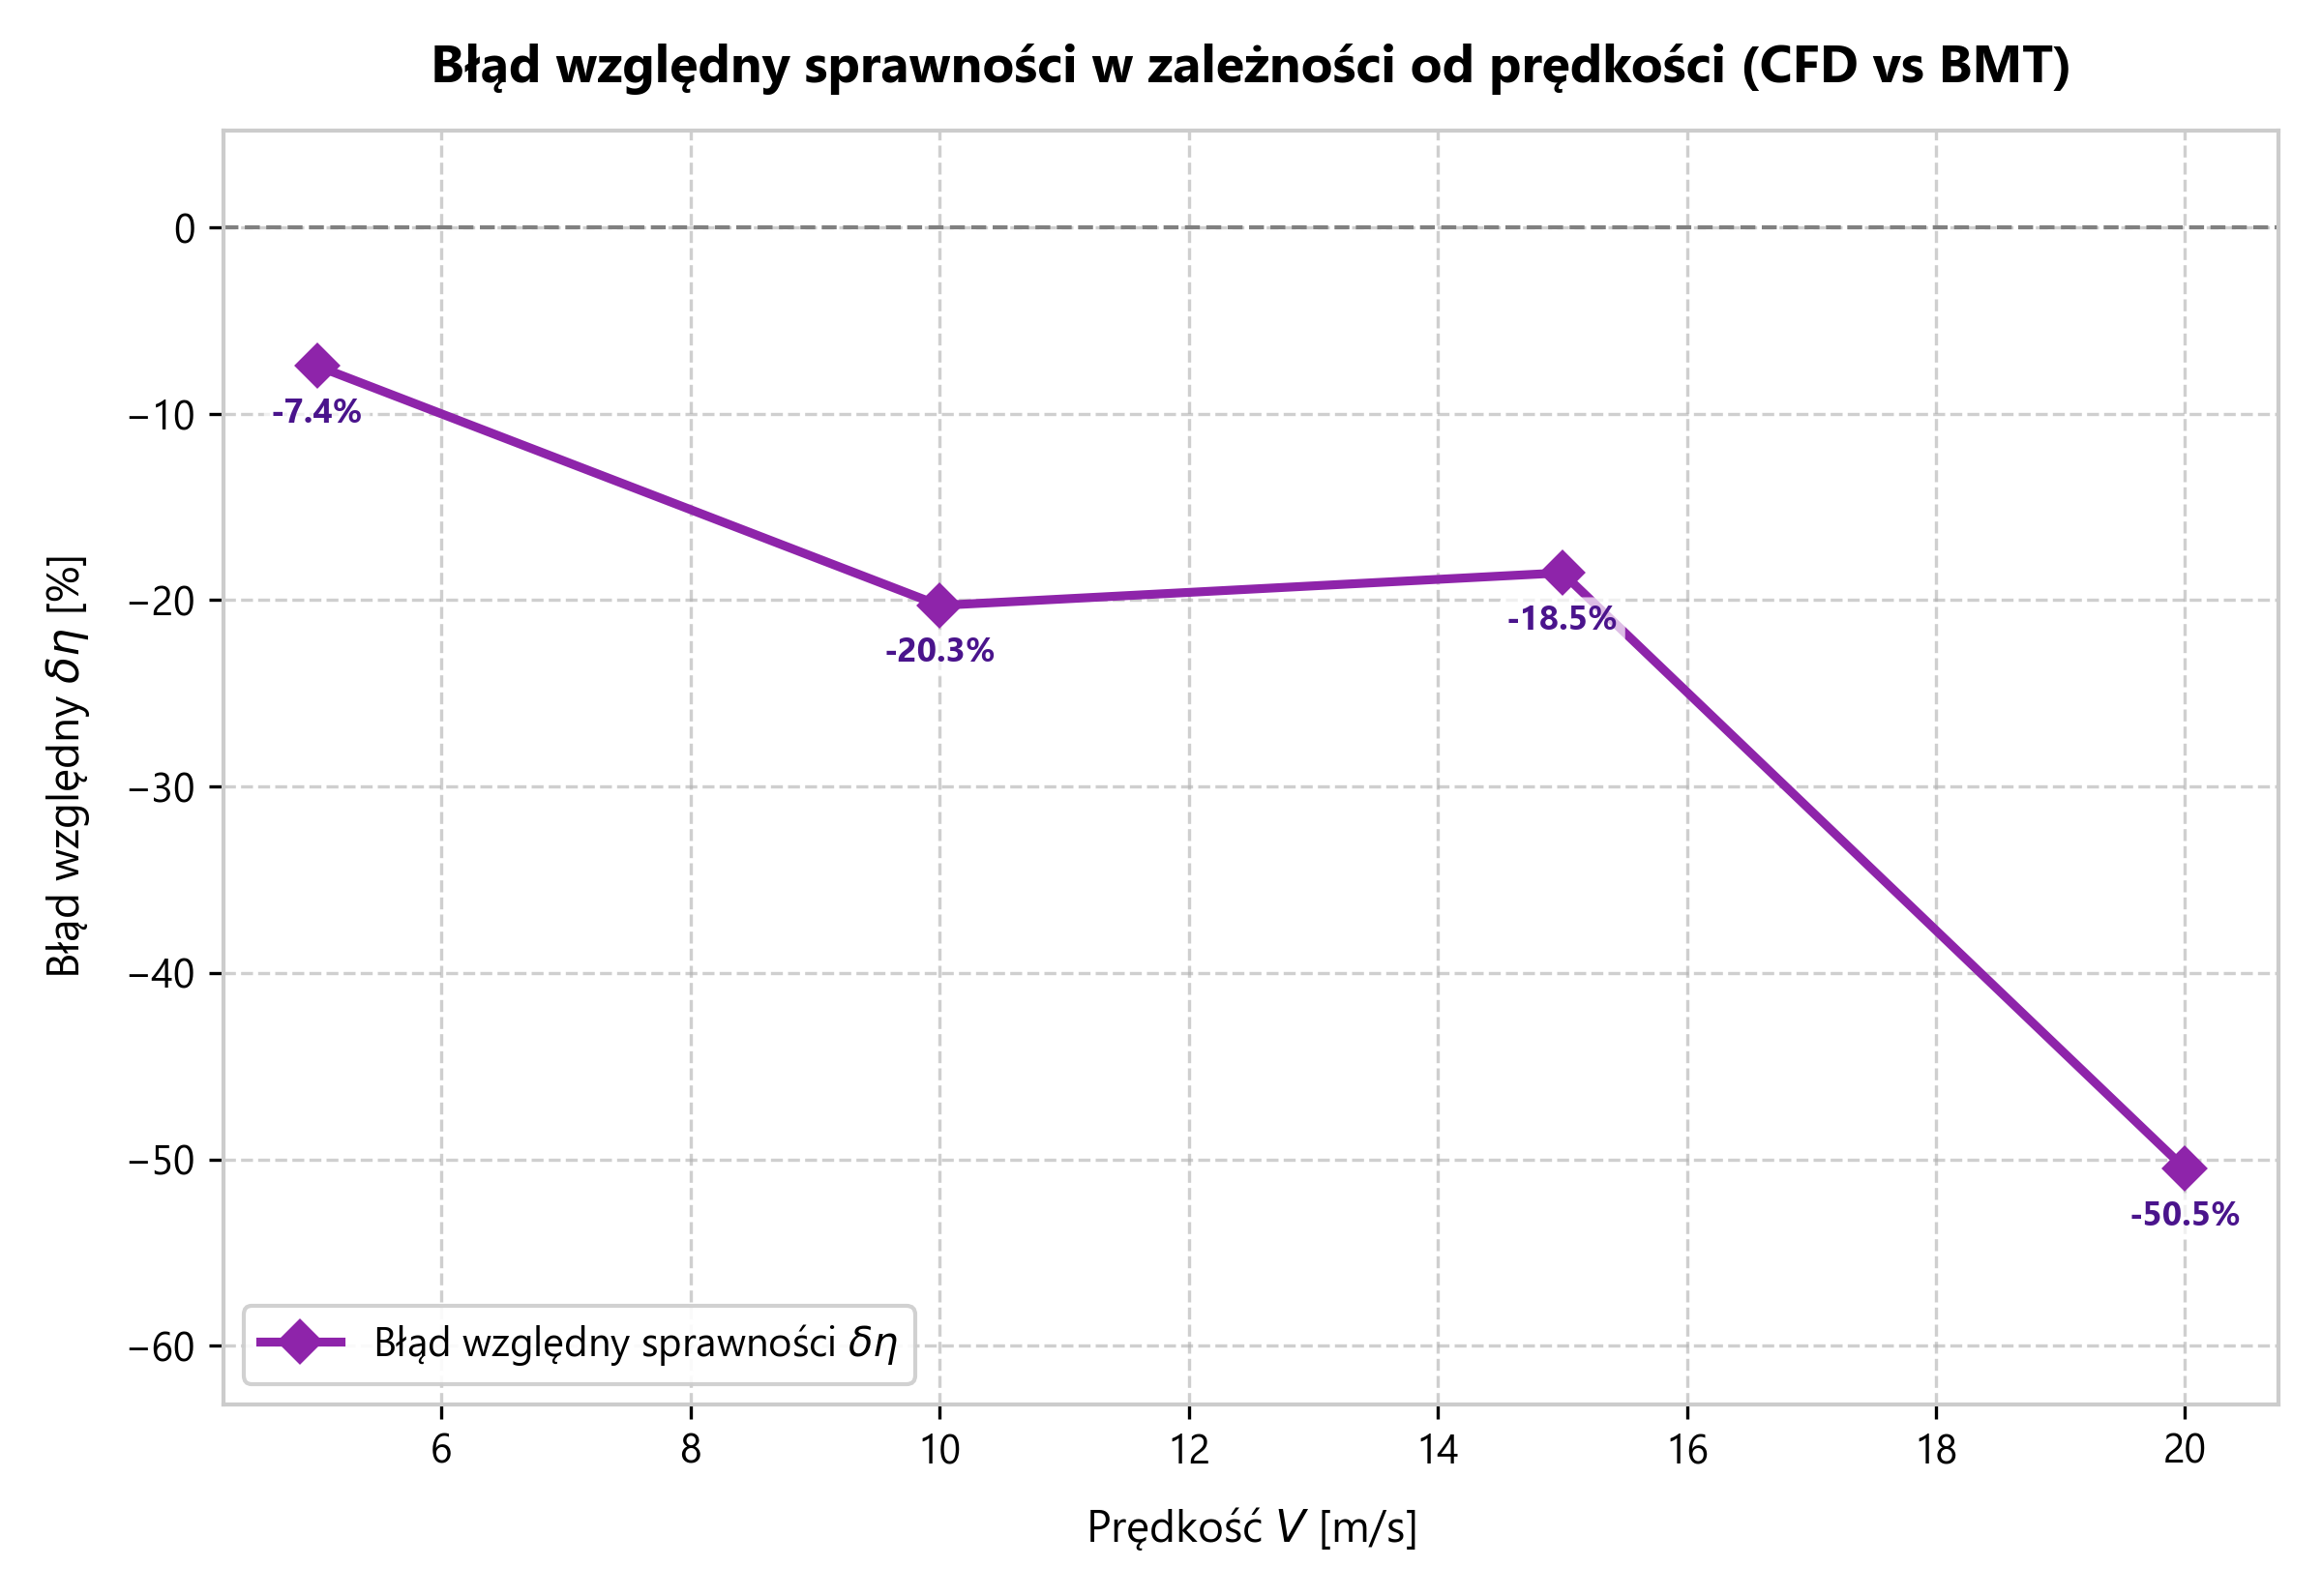
\includegraphics[width=.82\linewidth]{wykresy/10_blad_wzgledny_sprawnosc.png}
		\caption{Błąd względny sprawności \(\delta\eta\) w funkcji prędkości napływu \(V\).}
		\label{fig:blad_sprawnosc}
	\end{figure}
	
	\subsubsection{Porównanie ciągu}
	Dla prędkości \(V_\infty = 30\) m/s, gdzie śmigło pracuje w trybie hamulcowym (ciąg ujemny), wyniki CFD porównano z obliczeniami metody BMT. Uzyskana różnica względna wynosi ok. \(+6{,}6\%\) (CFD: \(-9{,}28\) N, BMT: \(-9{,}94\) N), co jest wartością bardzo dobrą dla tego trudnego reżimu przepływu. W zakresie małych i średnich prędkości napływu symulacja CFD przewiduje niższe wartości ciągu niż metoda BMT, przy czym rozbieżności względne zawierają się w przedziale ok. 30--63\%. Wynika to z uproszczeń modelu analitycznego oraz zjawisk trójwymiarowych, których metoda BMT nie uwzględnia. Skok błędu względnego do ok. \(-166\%\) przy \(V_\infty = 25\) m/s wynika z przejścia przez zero ciągu BMT (bardzo mały mianownik błędu), a nie z rzeczywistego wzrostu rozbieżności bezwzględnej.
	
	\subsubsection{Porównanie momentu obrotowego}
	Dla prędkości \(V_\infty = 25\) m/s moment obrotowy obu metod przyjmuje niewielkie wartości ujemne (\(Q_{\text{CFD}} = -0{,}033\) Nm, \(Q_{\text{BMT}} = -0{,}035\) Nm), a błąd względny wynosi ok. \(+4{,}8\%\), co potwierdza dobrą zgodność w okolicy zmiany znaku. W zakresie pracy dodatniej (5--20 m/s) CFD przewiduje moment niższy o ok. 25--38\% niż BMT. Największy błąd względny (+71,5\%) występuje przy \(V_\infty = 30\) m/s, gdzie obie metody przewidują niewielkie wartości ujemne (\(-0{,}20\) Nm vs \(-0{,}70\) Nm).
	
	\subsection{Podsumowanie analizy CFD}
	Przeprowadzone symulacje CFD pozwoliły na wyznaczenie charakterystyk aerodynamicznych śmigła dwułopatowego o średnicy \SI{0.5}{\meter} dla zakresu prędkości napływu od 0 do \SI{30}{\meter\per\second} przy stałej prędkości obrotowej \SI{3000}{rpm}. Zastosowanie metody MRF oraz modelu turbulencji \(k-\omega\) SST zapewniło stabilną zbieżność obliczeń oraz uzyskanie wiarygodnych wyników. Uzyskane charakterystyki wykazują zgodny z fizyką przebieg: ciąg maleje ze wzrostem prędkości napływu od 19,08 N w warunkach statycznych do \(-9{,}28\) N przy \(V_\infty = 30\) m/s, a maksymalna sprawność ok. 67\% jest osiągana przy \(V_\infty = 15\) m/s. W zakresie pracy hamulcowej wyniki CFD pozostają w dobrej zgodności z obliczeniami BMT (błąd względny ciągu ok. \(+6{,}6\%\)), co potwierdza poprawność modelu.
	
	\subsection{Analiza rozbieżności między metodami}
	Porównanie wyników metod BMT i CFD ujawnia systematyczne rozbieżności, których źródła można podzielić na trzy grupy:
	\begin{itemize}
		\item \textbf{Uproszczenia metody BMT}: metoda elementów łopaty i pędu opiera się na założeniu dwuwymiarowego przepływu na każdym przekroju łopaty, nie uwzględnia w pełni efektów trójwymiarowych -- m.in. przepływów promieniowych, stref zwartego wiru końcowego oraz interakcji łopaty ze strugą. W rezultacie metoda BMT często zawyża ciąg i moment w zakresie małych prędkości napływu, co odpowiada obserwowanemu tu systematycznemu ujemnemu błędowi względnemu CFD (30--63\% mniejsze wartości w zakresie 0--20 m/s).
		\item \textbf{Ograniczenia symulacji CFD}: model MRF jest uproszczeniem, w którym łopaty nie obracają się względem domeny, a pole przepływu jest ustalone w wirującym układzie odniesienia; nie odtwarza to w pełni niestacjonarnych efektów rzeczywistego wirnika. Wpływ na wyniki mają również ustawienia solvera (schematy dyskretyzacji), jakość siatki oraz kryteria zbieżności. Lokalnie obniżona ortogonalność siatki (0,045) może dodatkowo ograniczać dokładność rozwiązania w obszarach dużych gradientów.
		\item \textbf{Kwestie metodologiczne porównania}: duże błędy względne przy \(V_\infty = 25\) m/s nie odzwierciedlają faktycznej rozbieżności bezwzględnej, lecz wynikają z dzielenia przez bardzo małą wartość referencyjną w okolicy zmiany znaku ciągu. Podobnie błąd momentu +71,5\% przy 30 m/s dotyczy niewielkich wartości bezwzględnych i jest wrażliwy na różnice modelowe.
	\end{itemize}
	Ocena dokładności obu metod wymaga ustalenia wartości referencyjnej. W przypadku prostych geometrii i klasycznych powietrzy o znanej geometrii łopat, dobrze skalibrowana metoda BMT daje wyniki wystarczająco dokładne przy bardzo małym koszcie obliczeniowym. Symulacja CFD jest natomiast bardziej uniwersalna: uwzględnia rzeczywisty, trójwymiarowy charakter przepływu, efekt wirowy za łopatą oraz efekty lepkości, przez co może być dokładniejsza w przypadkach, w których BMT zawodzi, np. przy znacznym obciążeniu, w pobliżu opływu bliskiego oderwania oraz w zakresie pracy hamulcowej. Jednakże dokładność CFD jest silnie zależna od jakości siatki, doboru modelu turbulencji i poprawności warunków brzegowych, dlatego w niniejszym badaniu, na podstawie zgodności wyników w zakresie hamulcowym oraz fizycznie spójnych przebiegów charakterystyk, za wiarygodniejszą uznano metodę CFD, zalecając jednocześnie jej walidację z danymi eksperymentalnymi lub niezależnymi obliczeniami (np. metoda panelową lub niestacjonarnym uruchamianiem solvera).
	
	\newpage
	\section{Wnioski końcowe}
	\begin{enumerate}
		\item Metoda BMT pozwoliła na szybkie oszacowanie podstawowych charakterystyk aerodynamicznych śmigła, takich jak ciąg, moment obrotowy, moc i sprawność, w funkcji prędkości lotu.
		\item Symulacje CFD wykonane w programie ANSYS Fluent uzupełniły zestaw wyników o punkty pracy w całym zakresie prędkości napływu 0--30 m/s, co umożliwiło pełny opis charakterystyk śmigła, w tym punkt statyczny oraz zakres hamulcowy.
		\item Zaobserwowano, że dla prędkości \(V_\infty > 20\) m/s śmigło przechodzi w tryb hamulcowy (ciąg ujemny), co jest zjawiskiem fizycznie poprawnym i zostało odwzorowane przez obie metody.
		\item Największa sprawność śmigła, wynosząca ok. 67\%, została osiągnięta dla prędkości napływu 15 m/s. W zakresie małych i średnich prędkości napływu symulacja CFD przewiduje niższe wartości ciągu niż metoda BMT (o ok. 30--63\%), co wynika z uproszczeń modelu analitycznego oraz efektów trójwymiarowych nieuwzględnianych przez BMT.
		\item W zakresie pracy hamulcowej (\(V_\infty = 30\) m/s) błąd względny ciągu CFD względem BMT wynosi zaledwie ok. \(+6{,}6\%\), co wskazuje na dobrą zgodność obu metod w tym reżimie przepływu. Duże błędy względne w okolicy 25 m/s wynikają z dzielenia przez niemal zerową wartość referencyjną, a nie ze znaczących różnic bezwzględnych.
		\item Mimo że jakość siatki (minimalna ortogonalność na poziomie 0,045) odbiega od zaleceń, symulacje wykazały stabilną zbieżność, co sugeruje, że lokalnie słaba jakość siatki nie wpłynęła znacząco na wyniki.
		\item Symulacja CFD uwzględnia trójwymiarowe i lepkie efekty przepływu, dlatego uznano ją za metodę bardziej uniwersalną i wiarygodniejszą w rozpatrywanych zakresach pracy; ostateczna weryfikacja wymaga jednak porównania z danymi eksperymentalnymi lub niezależną metodą obliczeniową.
		\item W celu dalszej poprawy dokładności zaleca się przeprowadzenie badania niezależności od siatki (\textit{mesh independence study}), poprawę jakości siatki w obszarach dużych gradientów oraz rozważenie niestacjonarnego sformułowania solvera (\textit{sliding mesh}).
	\end{enumerate}
	
	\begin{thebibliography}{9}
		\bibitem{mrf_method} ANSYS, Inc., \textit{ANSYS Fluent Theory Guide}, release 2024 R2, Canonsburg, PA, USA, 2024, rozdz. 2 (Moving Reference Frames).
		\bibitem{ansys_mesh_quality} ANSYS, Inc., \textit{ANSYS Meshing User's Guide}, release 2024 R2, Canonsburg, PA, USA, 2024.
		\bibitem{glauert} H. Glauert, \textit{The Elements of Aerofoil and Airscrew Theory}. Cambridge, UK: Cambridge University Press, 1926.
		\bibitem{hage2024} C. Hage, T. Sophy, E. H. Aglzim, ,,A comprehensive study on the aerodynamic influence of stationary and moving obstacles on an isolated phantom DJI 3 UAV propeller'', \textit{The Journal of Engineering}, vol. 2024, nr 4, e12374, 2024, doi: 10.1049/tje2.12374.
		\bibitem{kutty2017} H. A. Kutty, P. Rajendran, ,,3D CFD simulation and experimental validation of small APC slow flyer propeller blade'', \textit{Aerospace}, vol. 4, nr 1, art. nr 10, 2017, doi: 10.3390/aerospace4010010.
		\bibitem{menter1994} F. R. Menter, ,,Two-equation eddy-viscosity turbulence models for engineering applications'', \textit{AIAA Journal}, vol. 32, nr 8, pp. 1598-1605, 1994, doi: 10.2514/3.12149.
		\bibitem{moriarty} P. J. Moriarty, A. C. Hansen, \textit{AeroDyn Theory Manual}, raport NREL/TP-500-36881. Golden, CO, USA: National Renewable Energy Laboratory, 2005.
		\bibitem{seeni2019} A. Seeni, ,,Aerodynamic performance characterization and static structural analysis of slotted propeller: part A -- effect of position'', \textit{Mathematical Modelling of Engineering Problems}, vol. 6, nr 4, pp. 611-624, 2019, doi: 10.18280/mmep.060417.
		\bibitem{sikirica2019} A. Sikirica, Z. \v{C}arija, L. Kranj\v{c}evi\'{c}, I. Lu\v{c}in, ,,Grid type and turbulence model influence on propeller characteristics prediction'', \textit{Journal of Marine Science and Engineering}, vol. 7, nr 10, art. nr 374, 2019, doi: 10.3390/jmse7100374.
	\end{thebibliography}

	\clearpage
	\listoffigures
	\clearpage
	\listoftables
\end{document}
